\documentclass[color=green,thmcnt=section,lang=cn,12pt]{elegantbook}
\usepackage{imakeidx}
\usepackage{graphicx}  %引用图片的宏包
\usepackage{float}
\usepackage{wrapfig}  %使用图文混排的宏包
% \usepackage{tikz} %绘图
% \usetikzlibrary{positioning} %为了实现相对位置的设定
% \usepackage{xcolor} %为了实现不同的颜色
\makeindex[title={术语索引(按拼音排序)},columns=3,intoc=true,columnseprule=true]
\title{实变函数讲义}
\author{LMH}
\date{\today}
\numberwithin{equation}{section}%公式按章节编号
\numberwithin{figure}{section}%图表按章节编号
\definecolor{highlight}{RGB}{196, 255, 211} %一种新的高亮颜色
%\renewcommand{\seename}{见:}
\newcommand{\RR}{\mathbb{R}}
\renewcommand{\RN}{\RR^n}
\newcommand{\QQ}{\mathbb{Q}}
\newcommand{\CC}{\mathbb{C}}
\newcommand{\ZZ}{\mathbb{Z}}
\newcommand{\NN}{\mathbb{N}}
\newcommand{\ee}{\varepsilon}
\newcommand{\any}{\forall \ }
\newcommand{\exi}{\exists \ }
\newcommand{\sothat}{\ \textrm{s.t.}\ }
\newcommand{\csf}[1]{\{#1_k\}_{k\in \ZZ_+}} %countable set family 变元为k的可数集族
\newcommand{\cu}[1]{\bigcup_{#1=1}^{\infty}} %countable union 可数并
\newcommand{\ci}[1]{\bigcap_{#1=1}^{\infty}} %countable intersection 可数交
\newcommand{\cs}[1]{\sum_{#1=1}^{\infty}} %countable sum 可数和
\newcommand{\linf}[1]{\liminf_{k\rightarrow \infty}#1_k} %liminf 下极限
\newcommand{\lsup}[1]{\limsup_{k\rightarrow \infty}#1_k} %limsup 上极限
\newcommand{\li}[1]{\lim_{k\rightarrow \infty}#1_k} %lim 极限
\newcommand{\mx}[1]{\textrm{m}^*(#1)} %外测度m*
\newcommand{\lcover}{\textrm{L-cover}} %L-cover 
\newcommand{\kecef}[1]{\{#1_k:X\to [-\infty,\infty]\}_{k\in\ZZ_+}} %可测函数列
\newcommand{\jd}[1]{#1=\sum_{i=1}^{n}a_i\chi_{A_i}} %简单函数
\newcommand{\ff}[1]{#1:X\to [0,\infty]} %非负函数
\newcommand{\jdint}{\sum_{i=1}^{n}a_i\mu(A_i)} %简单函数积分
\newcommand{\ffint}[1]{\sup_{0\leq s \leq #1}\sum_{i=1}^{n}a_i\mu(A_i)$\ \ $(s=\sum_{i=1}^{n}a_i\chi_{A_i})} %非负函数积分
\newcommand{\ffinte}[1]{\sup_{0\leq s \leq #1}\sum_{i=1}^{n}a_i\mu(A_i\cap E)$\ \ $(s=\sum_{i=1}^{n}a_i\chi_{A_i})}
\newcommand{\normp}[2]{\Vert #1 \Vert_{#2}}
\newcommand{\p}[1]{(第\pageref{#1}页)}
\newcommand{\refp}[1]{\ref{#1}\p{#1}}
\newcommand{\bi}[2]{\colorbox{highlight}{\textbf{\textcolor[RGB]{14,14,94}{#1}}}\index{#2@#1} \label{#2}} %方便添加概念索引的命令
\newcommand{\holder}{\textrm{Hölder}}
%-------------------------------------------%
\cover{cover.jpg}
\begin{document}
\maketitle %标题
\tableofcontents %目录

\chapter{Lebesgue测度与可测函数}
%%%%%%%%%%%%%%%%%%%%%%%%%%%%%%%%%%%%%%%%%%%%%%%%%%%%%%%%%%%%%%%%%%%%%%%%%%%%
\section{Lebesgue测度的基本概念}\label{Lebesguecedudejibengainian}
对于$\RN$中的集合$E$,我们用可数个开矩体$$\csf{I}=\{(a_{1,k},b_{1,k})\times \cdots \times (a_{n,k},b_{n,k})\}_{k\in \ZZ_+}$$
从外部进行逼近,使得$E\subseteq \cu{k}I_k.\ $这些矩体全体称为$E$的一个\bi{L-cover}{lcover}.\ 
记$$\mx{E}=\inf \{\sum_{k=1}^{\infty}|I_k|: \csf{I}\text{为E的}\lcover \},$$称它为$E$的
\bi{Lebesgue外测度}{lebesguewaicedu},其中$|I_k|=\prod_{i=1}^{n}(b_{i,k}-a_{i,k})$表示$I_k$的体积。\par\,

\begin{remark}
\begin{enumerate}
    \item  外测度有非负性($\mx{A}\geq 0,\ \any A\subseteq \RN$)、单调性(若$A\subseteq B$,则$\mx{A}\leq \mx{B}$)、
可列次可加性(对于$\RN$中任意可数个集合$\csf{A},\ \mx{\cu{i}A_i}\leq \cs{i}\mx{A_i}$)。
\item 从空集的外测度为0可以看出$ \mx{\cup_{i}^{n}{A_i}}\leq \sum_{i=1}^{n}\mx{A_i}$.
\item 单点集外测度为0,根据可列次可加性,可数点集的外测度为0.
\item $\RN$中维数不大于$n-1$的超平面外测度为0.
\end{enumerate}
\end{remark}
\ 


\begin{note}
    不可数点集的外测度未必非零,比如Cantor集(例\refp{ceduweilingdebukeshudianji})。
\end{note}
\ 


从上面定义不难看出,外测度是对$\RN$中集合大小的一种描述。对于我们容易想象到的集合(比如长方体),它的外测度就是它的体积。

\begin{proposition}
    对于$\RN$中任何一个开矩体I,总有$\mx{I}=|I|=\mx{\overline{I}}.$
\end{proposition}
\begin{proof}
    这个命题看似显然,但证明并不算简单。我们先说明$\mx{\overline{I}}=|I|.$


    首先,$\any \ee>0,\ \exi \mbox{开矩体}A\supseteq I,\sothat 0<|A|-|I|<\ee.$
    注意$\{A\}$是$\overline{I}$的一个L-cover,故$\mx{\overline{I}}\leq |A|<|I|+\ee$.
    由$\ee$的任意性,$\mx{\overline{I}}\leq |I|.\ $另一方面,$\overline{I}$是$\RN$中
    有界闭集,从而是紧集。任给$\overline{I}$的一个$\lcover\ \csf{A}$,这个开覆盖存在有限子覆盖,
    不妨设$\cup_{i=1}^tA_i\supseteq \overline{I}$,
    那么$\cs{i}|A_i| \geq \sum_{i=1}^{t}|A_i|\geq |I|$,这说明$\mx{\overline{I}}\geq |I|$.\ 
    综上,有$\mx{\overline{I}}=|I|.$\ 


    $\{I\}$为I的一个L-cover,故$\mx{I}\leq |I|.\ $另一方面,$\mx{I}\geq \mx{\overline{I}}-\mx{\overline{I}-I}=
    \mx{\overline{I}}=|I|$(注意到$\overline{I}-I$为有限个$n-1$维平面的并),故$\mx{I}=|I|=\mx{\overline{I}}.$
\end{proof}
\ 


外测度类似于集合的``体积'',我们自然要问,两个不相交的集合之并的外测度,是否是它们各自的外测度之和?
一般来说我们不能保证(不可测集的定义给出了反例的存在性),但我们有所谓的``分离可加性''\index{fenlikejiaxing@分离可加性},即:
\begin{proposition}[分离可加性]\label{fenlikejiaxing}
    设$E_1,E_2\subseteq \RN,\ \mbox{两集合距离}\ d(E_1,E_2)>0$,那么$\mx{E_1\cup E_2}=\mx{E_1}+\mx{E_2}$.
\end{proposition}
\begin{proof}
    只用证明左边不小于右边。不妨设左边有界。我们只需要注意到下面的事实:规定L-cover中每个
    矩体的边长都小于某一常数后,这些L-cover中矩体体积和的下确界依然是外测度。这是因为,$\any \ee>0$,
    我们选定$E=E_1\cup E_2$的一个L-cover\ $\csf{I}$,使得$\cs{k}|I_k|<\mx{E}+\ee$后,可以对每个$I_k$进行分割,得到若干个
    边长小于某一常数的矩体。把这些矩体边长扩大到原来的$\lambda$倍($\lambda$很接近1),再取内部,就得到若干个新的
    开矩体,它们全体是$I_k$的L-cover。对每个$k$类似处理,我们得到了一个新的L-cover,其中矩体的体积和与$\cs{k}|I_k|$很接近,
    但所有矩体的边长小于某一常数。


    下面我们假设这个常数是$d(E_1,E_2)/{\sqrt{n}}$,那么得到的L-cover(设为$\csf{A}$)中每个矩体不可能同时
    与$E_1,\ E_2$相交。根据上面的讨论,我们可以要求$\cs{k}|A_k|<\mx{E}+\ee$,将$\csf{A}$分为$E_1$的$\lcover$和$E_2$的$\lcover$两部分即可。
\end{proof}
\ 


外测度还具有``平移不变性''\index{pingyibubianxing@平移不变性},即$\mx{E+\{x_0\}}=\mx{E}$,其中
$E+\{x_0\}=\{x+x_0:\ x\in E\}$,证明从略。


由于对于一般的两个不相交的集合,它们外测度之和未必是它们的并集的外测度,
这不符合我们的直观感受。
我们先假设有这样一个``可测集''类,它们中两个不交集合的外测度之和恰好是它们的并集的外测度。
下面的问题是,这样的``可测集''类应该如何定义。


首先,我们要求任意矩体$I\subset \RN$是可测集。如果$E\subset \RN$是可测集,
那么$\mx{I\cap E}+\mx{I\cap E^c}=\mx{I}$.\ 事实上,我们这样要求已经足够了。

\begin{definition}[Lebesgue可测集]\label{lebesguekecejidingyi}
    若对任一开矩体I,都有$\mx{I\cap E}+\mx{I\cap E^c}=\mx{I}$,我们就称
    E为\bi{Lebesgue可测集}{lebesguekeceji}。记可测集全体为$\mathfrak{M}$。
\end{definition}
事实上,这个定义等价于:\textbf{对任一集合T,都有$\mx{T\cap E}+\mx{T\cap E^c}=\mx{T}$},
证明是容易的(考虑T的$\lcover$即可)。我们把这里的T称为\bi{试验集}{shiyanji}。


容易证明,零测集(即外测度为0的集合)是Lebesgue可测集。零测集的任一子集是零测集,进而是Lebesgue可测集(若我们选取其它的测度则未必,见定义\ref{cedukongjiandewanbeihua})。
根据定义,我们同样不难证明下面命题:
\begin{proposition}\label{youxiankejiaxing}
    \begin{itemize}
        \item 若S为可测集,$A\subseteq S,\ B\subseteq S^c$,则$\mx{A\cup B}=\mx{A}+\mx{B}$.
        \item 设$E_1,E_2$为不交可测集,那么$\any T\subseteq \RN,\ \mx{T\cap(E_1\cup E_2)}=\mx{E_1\cap T}+\mx{E_2\cap T}$.
        \item 设$E_1,E_2$为不交可测集,那么$\mx{E_1\cup E_2}=\mx{E_1}+\mx{E_2}$.
    \end{itemize}
\end{proposition}
这个命题说明了,我们上面所定义的可测集对外测度确实满足``有限可加性'',即有限个不相交的可测集的并集的
外测度,等于它们各自的外测度之和。事实上可测集还对外测度满足``可列可加性'',这在后面会证明。


下面我们对可测集的性质作简单探讨。空集的外测度为0,是可测集。可测集的补集根据定义也是可测集。
两个可测集$E_1,E_2$的并集可测,这注意到$\any T \subseteq \RN$, \begin{align*}
   & \mx{(E_1\cup E_2)\cap T}+\mx{(E_1\cup E_2)^c\cap T}\\
    &\leq \mx{E_1\cap T}+\mx{(E_2\cap E_1^c)\cap T}+\mx{(E_1\cup E_2)^c\cap T}\\
    &=\mx{E_1\cap T}+(\mx{(T\cap E_1^c)\cap E_2}+\mx{(T\cap E_1^c)\cap E_2^c})\\
    &=\mx{E_1\cap T}+\mx{E_1^c\cap T}=\mx{T}
\end{align*}即可。接下来不难看出,\textbf{有限个可测集的并、交都可测}。

\begin{proposition}\label{kecejixingzhi1}
    设$\csf{E}$为不交可测集列,那么$\any T\subseteq \RN,\ \mx{T\cap (\cu{n}E_n)}=\cs{n}\mx{T\cap E_n}$.
\end{proposition}
\begin{proof}
    只用证明$\mx{T\cap (\cu{n}E_n)}\geq \cs{n}\mx{T\cap E_n}$,根据命题\ref{youxiankejiaxing}和上面的讨论不难看出,
           \begin{align*}
             \mx{T}&=\mx{T\cap (\cup_{i=1}^{n}E_i)^c}+\mx{T\cap(\cup_{i=1}^{n}E_i)}\\&=\mx{T\cap (\cup_{i=1}^{n}E_i)^c}+\sum_{i=1}^{n}\mx{T\cap E_i}\\
             &\geq \mx{T\cap (\cup_{i=1}^{\infty}E_i)^c}+\sum_{i=1}^{n}\mx{T\cap E_i}
           \end{align*}
    令n趋于无穷,得到
        $\mx{T} \geq \mx{T\cap (\cup_{i=1}^{\infty}E_i)^c}+\sum_{i=1}^{\infty}\mx{T\cap E_i}$
    .\ 用$T\cap (\cu{n}E_n)$替代$T$就完成了证明。
\end{proof}
\ 



\begin{definition}[$\sigma$代数]\label{sdaishu}
    设A为一个集合,$\rho(A)$为它的幂集,即所有子集构成的集合。
    设$\Gamma \subseteq \rho(A)$,如果:


        \quad  (1)\  $\emptyset \in \Gamma$;\ (2)\ 
        $A\in \Gamma \Rightarrow A\in \Gamma^c$(对取补封闭);\ (3)\ 
        $\any i\in \ZZ_+,\ A_i \in \Gamma \Rightarrow \cu{i}A_i\in \Gamma$(对可列并封闭)


    就称$\Gamma$为一个\bi{$\sigma$-代数}{sigmadaishu}。上述定义第三条也可以改为对可列交封闭。
    设$\Sigma \subseteq \rho(A)$,称包含$\Sigma$的最小$\sigma$-代数为
    由$\Sigma$生成的$\sigma$-代数。$\RN$中全体开集生成的$\sigma$-代数记作$\mathfrak{B}$,称为\bi{Borel代数}{boreldaishu},$\mathfrak{B}$中元素称为\bi{Borel集}{borelji}。
\end{definition}


\begin{proposition}\label{mshisigmadaishu}
    可测集全体$\mathfrak{M}$是一个$\sigma$-代数.
\end{proposition}
\begin{proof}
    根据定义和前面的讨论,我们只用再证明$\mathfrak{M}$对可列并封闭。设$\csf{E}$为一列可测集,设$$E=\cu{i}E_i,\ E_{1}^{'}=E_1,\ E_i^{'}=E_i-\cup^{i-1}_{k=1}E_k\ (i\geq 2),$$
    根据上面的讨论, $E_n^{'}\ (n\in \ZZ_+)$为不交的可测集。
    设 $\widetilde{E_n}=\cup_{i=1}^n E_i^{'}$,那么
    $\widetilde{E_n} \ (n\in \ZZ_+)$均为可测集,并且单增地趋于E。
    我们要说明$\any T\subseteq \RN,\ \mx{T}\geq \mx{T\cap E^c}+\mx{T\cap E}$.\ 
    注意$$\any n\in \ZZ_+, \ \mx{T}=\mx{T\cap \widetilde{E_n}}+\mx{T\cap \widetilde{E_n}^c}=\sum_{i=1}^{n}\mx{T\cap E_i^{'}}+\mx{T\cap \widetilde{E_n}^c},$$(这一步用了命题\ref{youxiankejiaxing}的结论),显然RHS\,$\geq \sum_{i=1}^{n}\mx{T\cap E_i^{'}}+\mx{T\cap E^c}$,
    令n趋于无穷,并注意外测度的可列次可加性,得到
    % 根据命题\ref{kecejixingzhi1}
    $$\mx{T}\geq \sum_{i=1}^{\infty}\mx{T\cap E_i^{'}}+\mx{T\cap E^c}\geq \mx{\cu{i}(T\cap E_i^{'})}+\mx{T\cap E^c}=\mx{T\cap E}+\mx{T\cap E^c},$$从而证毕。
\end{proof}
\ 


\begin{definition}[正测度]\label{zhengcedudingyi}
    设X为非空集合,$\Gamma \subseteq \rho(X)$为一个$\sigma$-代数,$\mu$为定义在$\Gamma$上的一个集合函数。如果$\mu$满足下面三个性质,
    就称它为$\Gamma$上的\bi{正测度}{zhengcedu}:
    \begin{enumerate}[(1)]
        \item $\any A\in \Gamma,\ \mu(A)\geq 0$
        \item $\mu(\emptyset)=0$
        \item 可列可加性:对$\Gamma$中两两不交的集合列$\csf{E}$,有$\mu(\cu{i}E_i)=\cs{i}\mu(E_i)$
    \end{enumerate}
    $\Gamma$中的元素此时也称为\bi{可测集}{keceji},$(X,\Gamma)$称为\bi{可测空间}{kecekongjian},$(X,\Gamma,\mu)$称为\bi{测度空间}{cedukongjian}。
\end{definition}
容易看出正测度也具有\textbf{有限可加性、单调性}($A,\ B\in \Gamma,\ A\subseteq B \Rightarrow \mu(A)\leq \mu(B)$)、\textbf{可列次可加性}。


设$\csf{E}$为一簇不交的Lebesgue可测集列,根据命题\ref{mshisigmadaishu},$E=\cu{k}E_k$也可测,并且从命题\ref{kecejixingzhi1}不难看出,对任意试验集T,有
$\mx{T}=\mx{T\cap E}+\mx{T\cap E^c}=\sum_{i=1}^{\infty}\mx{T \cap E_i}+\mx{T\cap E^c}$.
\ 取$T=E$,就得到$\mx{E}=\cs{i}\mx{E_i}$.\ 于是$\textrm{m}^{*}$为$\mathfrak{M}$上的正测度,我们称其为
\bi{Lebesgue测度}{lebesguecedu},记作m.


正测度具有所谓的\bi{从下连续性}{congxialianxuxing}和\bi{从上连续性}{congshanglianxuxing}。
前者指对单增集合列$\csf{E},$有$$ \mu(\lim_{k\rightarrow \infty}E_k)=\lim_{k\rightarrow \infty}\mu(E_k),$$
后者指对单减的、测度小于无穷的集合列$\csf{E}$,同样的结论成立。\par\,

\begin{remark}
    这里集合列的单调性和极限是类比数列的情况,
集合列的单调性将偏序关系从``<''改为``$\subseteq$''即可。


集合列$\csf{A}$的上下确界分别定义为$\cu{k}A_k$和$\ci{k}A_k$;


\bi{集合列的上极限}{jiheliedeshangjixian}定义为$$\limsup_{i\rightarrow \infty} A_i=\inf_{n\geq 1} \sup\{A_i\}_{i=n}^{\infty}=\ci{n}\cup_{i=n}^{\infty}A_i,$$
\bi{集合列的下极限}{jiheliedexiajixian}定义为$$\liminf_{i\rightarrow \infty} A_i=\sup_{n\geq 1} \inf\{A_i\}_{i=n}^{\infty}=\cu{n}\cap_{i=n}^{\infty}A_i.$$
当上下极限相等时,集合列$\csf{A}$的极限存在,记作$\lim_{k\rightarrow \infty}A_k.\ $容易看出,单调集合列的极限总存在。
\end{remark}


正测度的从上连续性、从下连续性
证明是容易的,比如从上连续性证明只需将$\cu{i}E_i$拆为$\cu{i}(E_i-E_{i-1}),\ E_0=\emptyset$即可。
事实上,外测度(虽然不是正测度)也具有从下连续性,这在例\refp{waicedudecongxialianxuxing}中会给出证明。

\begin{proposition}[测度论的Fatou引理]\label{cedulundefatouyinli}
    设$\csf{E}$为测度空间$(X,\Gamma,\mu)$中的可测集列,则
        $\mu(\liminf_{n  \to \infty}E_n)\leq \liminf_{n\rightarrow \infty}\mu(E_n)\mbox{;当}\cup_{n=1}^{\infty}  E_n\ \mbox{测度小于无穷,}\mu(\limsup_{n  \to \infty} E_n)\geq \limsup_{n\rightarrow \infty}\mu(E_n)$.
\end{proposition}
\begin{proof}
    对于前一式,设$H_n=\cap_{k=n}^\infty E_k$,它单调递增,
    根据测度的从下连续性,有
    \begin{equation*}
        \mu(\linf{E})=\mu(\lim_{n\rightarrow \infty}H_n)=\lim_{n\rightarrow \infty}\mu(H_n)=\liminf_{n\rightarrow \infty}\mu(H_n)\leq \liminf_{n\rightarrow \infty}\mu(E_n).
    \end{equation*}    
    对于后一式,设$A_n=\cup_{k=n}^\infty E_k$,它单调递减,且第一项测度小于无穷。
    根据测度的从上连续性,有
    \begin{equation*}
        \mu(\lsup{E})=\mu(\lim_{n\rightarrow \infty}A_n)=\lim_{n\rightarrow \infty}\mu(A_n)=\limsup_{n\rightarrow \infty}\mu(A_n)\geq \limsup_{n\rightarrow \infty}\mu(E_n).
    \end{equation*}
\end{proof}
\ 


最后给出一个在概率论中常见的引理。
\begin{lemma}[Borel-Cantelli]\label{bcyinli}
    \index{bcyinli@Borel-Cantelli引理}
    如果可数个事件发生的概率总和有限,那么它们之中有无限多个同时发生的概率等于零。
\end{lemma}
\begin{proof}
    设事件列$\csf{A}$满足$\cs{k}\mathbb{P}(A_k)\leq \infty$,$\csf{A}$中有无穷多个同时发生,等价于
    $\any k\in \ZZ_+,\ \exi n_k\geq k,\ A_{n_k}$发生了,即$\ci{k}\cup_{n=k}^{\infty}A_n=\limsup_{k\rightarrow \infty}A_k$发生了。
    事实上,对于任意正测度$\mu$,只要$\cs{n}\mu(A_n)\leq \infty$,我们有
    \begin{equation*}
        \mu(\limsup_{k\rightarrow \infty}A_k)=\mu(\ci{k}\cup_{n=k}^{\infty}A_n)\leq \mu(\cup_{n=k}^{\infty}A_n)\leq \sum_{n=k}^{\infty}\mu(A_n)\rightarrow 0\ (k\rightarrow \infty).
    \end{equation*}
    从而证毕。
\end{proof}
\ 


%%%%%%%%%%%%%%%%%%%%%%%%%%%%%%%%%%%%%%%%%%%%%%%%%%%%%%%%%%%%%%%%%%%%%%
\newpage\section{Lebesgue可测集与不可测集}
Lebesgue可测集除了矩体之外,还包含哪些集合?Lebesgue可测集有哪些性质?如何构造不可测集?下面我们将对这些问题进行探讨。
\begin{theorem}
   可测集包含所有Borel集。
\end{theorem}

\begin{proof}
    只用证明任何一个闭集$F\subseteq \RN$都可测,再根据命题\ref{mshisigmadaishu}知可测集包含所有Borel集。
取试验集T,以及$$F_k=\{x\in T-F\ :\ d(x,(T-F)^c)\geq 1/k\}$$(如下图所示),则由外测度的分离可加性(命题\refp{fenlikejiaxing}),知:
$$\mx{T}\geq \mx{F_k\cup (T\cap F)}=\mx{F_k}+\mx{T\cap F}.$$
如果我们能够证明,$\lim_{k\rightarrow \infty}\mx{F_k}=\mx{\lim_{k\rightarrow \infty}F_k}$,
再由$F_k\rightarrow T-F\ (k\rightarrow \infty)$就得到$\mx{T}\geq \mx{T\cap F}+\mx{T\cap F^c}$,从而F可测。
我们只需证明,对任一非空闭集$F\subset \RN$,若$E\cap F=\emptyset$,$E_k=\{x\in E\ :\ d(x,F)\geq 1/k\}$,则$$\lim_{k\rightarrow \infty}\mx{E_k}=\mx{\lim_{k\rightarrow \infty}E_k}=\mx{E}.$$ 
这就是\bi{Caratheodory引理}{caratheodoryyinli}。


下面我们设$A_k=E_{k+1}-E_k$,注意到$E=E_{2k}\cup (\cup_{j=k}^{\infty}A_{2j})\cup (\cup_{j=k}^{\infty}A_{2j+1})$,两边取外测度,
并利用外测度的分离可加性(注意$\{A_{2j}\}_{j=k}^\infty$,$\{A_{2j+1}\}_{j=k}^\infty$中任两个集合的距离都大于0),得到
$$\mx{E}\leq \mx{E_{2k}}+\sum_{j=k}^{\infty}\mx{A_{2j}}+\sum_{j=k}^{\infty}\mx{A_{2j+1}}.$$注意单调有界序列的极限存在,并且等于任一子列的极限,
令k趋于无穷不难得到$\lim_{k\rightarrow \infty}\mx{E_k}\geq \mx{E}$(细节略去)。另一个方向是显然的,从而证毕。
\end{proof}
\ 


\begin{wrapfigure}{r}{0pt}
    \centering
    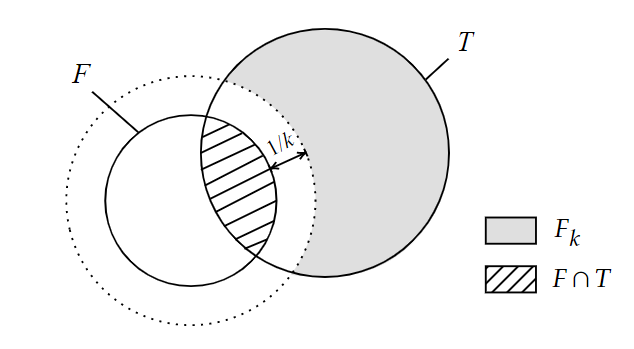
\includegraphics[height=4.5cm]{image/1.png}
    \caption{利用$F_k$逼近$T-F$}
\end{wrapfigure}


尽管可测集包含所有的Borel集,但也存在不是Borel集的可测集,详见例\refp{feiboreljidekeceji}。


我们接下来探讨可测集的性质。我们指出,\textbf{可测集和包含它的开集、在它其中的闭集在测度上可以非常接近}。
我们首先说明:对于$E\in \mathfrak{M},\ \any \ee>0,\ \exi$开集$ G\supseteq E,\sothat m(G-E)<\ee$.\ 事实上,
当$m(E)<\infty$时取G为E的一个L-cover$\csf{I}$之并$\cu{k}I_k$即可;当$m(E)=\infty$时考虑$E_k=E\cap B(0,k)$,对每个$E_k$取开集$G_k,\sothat m(G_k-E_k)<\ee/2^k$,令$G=\cu{i}G_i$即可。
与此同时,对E和G取补集易见$\any E\in \mathfrak{M},\ \any \ee>0,\ \exi F\subseteq E,\sothat m(E-F)<\ee$.\ 
事实上,对于可测集我们还有下面的刻画:

\begin{theorem}[Lebesgue可测集的刻画]\label{lebesguekecejidekehua}
    下面三个说法等价:
    \begin{enumerate}[(1)]
        \item E为Lebesgue可测集
        \item 存在\bi{$G_\delta$集}{gdeltaji}(即可数个开集之交)\ $H\supseteq E$,使$Z=H-E$为零测集(H称为E的\bi{等测包}{dengcebao})
        \item 存在\bi{$F_\sigma$集}{fsigmaji}(即可数个闭集之并)\ $K\subseteq E$,使$Z=E-K$为零测集(K称为E的\bi{等测核}{dengcehe})
    \end{enumerate}
\end{theorem}
\begin{proof}
    $(2)$或$(3)\Rightarrow (1)$:注意零测集可测,开集与闭集的可列交或可列并为Borel集,也可测,而可测集的并集可测;
    $(1)\Rightarrow (2)$:对可测集E,$\any k \in \ZZ_+,\ \exi $开集$G_k\supseteq E,\ \sothat m(G_k-E)<1/k.\ $取
    $H=\ci{k}G_k$即可。同理$(1)\Rightarrow (3)$。
\end{proof}
\ 


\begin{note}
    对于一般的集合E,容易证明:存在$G_\delta$集H,使$m(H)=\mx{E}$,此时我们也称H为E的等测包,
    但是未必有$H-E$为零测集。设$M\subseteq H,\ H-M\subseteq H-E$为可测集,则M可测且包含E,$m(H-M)=m(H)-\mx{M}\leq m(H)-\mx{E}=0$,
    故$H-E$的任何一个可测子集是零测集。
    \\ \ 
\end{note}

事实上,对于测度小于无穷的集合E,E为Lebesgue可测集等价条件还有:$$\mx{E}=\sup \{m(F)\ :\ F\subseteq E \ \mbox{为有界闭集}\},$$即:\textbf{E无论从外部用开集逼近,还是从内部用闭集逼近,结果是一致的}。
这一点也较为显然,我们设$G_\delta$集H是E的等测包,
那么对任意闭集$F\subseteq E$有$H-E\subseteq H-F,\ \mx{H-E}\leq \mx{H-F}=m(H-F)=m(H)-m(F)=\mx{E}-m(F)$可以任意小,故
$H-E$为零测集,根据定理\ref{lebesguekecejidekehua}知E可测。至于另一个方向,可以从下面的推论得出:

\begin{corollary}\label{kecejibeijinjibijin}
    设E为Lebesgue可测集,则$m(E)=\sup\{m(K)\ :\ K\subseteq E,\ K\ \mbox{为紧集}\}$.
\end{corollary}
\begin{proof}
    设$E_k=E\cap B(0,k)$,$\any\ee>0$,设闭集$F_k\subseteq E_k$满足$m(E_k-F_k)<\ee/2$,那么
    $F_k$是有界闭集,从而是紧集。由于$$\lim_{k\to\infty}m(E_k)=m(\lim_{k\to\infty}E_k)=m(E),$$若$m(E)<\infty$,易见存在$K$使得
    $m(E)<m(E_K)+\ee/2$,那么$m(E)<m(F_K)+\ee$,根据上确界的定义可知结论成立;若$m(E)=\infty$,那么任给$M>\ee$,存在$K$使得
    $m(E_K)>2M$,故$m(F_K)>2M-\ee>M$,从而$\sup\{m(K)\ :\ K\subseteq E,\ K\ \mbox{为紧集}\}=\infty$.
\end{proof}
\ 


\begin{example}[(外测度的从下连续性)]\label{waicedudecongxialianxuxing}
对于递增集合列$\csf{E}$,\ 有$\lim_{k \rightarrow \infty}\mx{E_k}=\mx{\li{E}}$;
一般来说,有$\mx{\linf{E}}\leq \liminf_{k\rightarrow \infty}\mx{E_k}$.\ 
\end{example}
\begin{proof}
    先证后一命题。
    设$E_k$的等测包为$H_k$,那么根据测度论的Fatou引理(\ref{cedulundefatouyinli}),我们有
    \begin{equation*}
        \liminf_{k \rightarrow \infty}\mx{E_k}=\liminf_{k \rightarrow \infty}\mx{H_k}\geq \mx{\liminf_{k \rightarrow \infty}H_k}\geq \mx{\liminf_{k \rightarrow \infty}E_k}
    \end{equation*}
    对于递增集合列,其下极限就是极限。故$\lim_{k\to\infty}\mx{E_k}\geq \mx{\li{E}}$,另一个方向根据$E_k\subseteq \cu{i}E_i$和外测度的单调性可见。
\end{proof}
\ 


\begin{example}[(平移不变性)]
    可测集E经过平移之后(比如说得到$E+\{a\}$)依然可测,且测度不变。
\end{example}
\begin{proof}
    由定理\ref{lebesguekecejidekehua}知$E=\ci{k}G_k-Z$,其中$G_k$为开集,Z为零测集。易见
    开集平移后还是开集,零测集平移后还是零测集,从而平移后的E依然是可测集。测度不变是显然的。
\end{proof}
\ 

\begin{proposition}\label{zhengcedujijihubaohanjuti}
    设E为测度大于0的Lebesgue可测集,则对任意$0<\lambda<1$,存在矩体I,$\lambda |I|<m(I\cap E)$.\ 
\end{proposition}
\begin{proof}
    不妨设$m(E)<\infty,\ $否则用$E\cap B(0,R)$代替E。我们从E的$\lcover$中寻找这样的矩体。对于任意给定的$0<\lambda<1$,我们待定$\ee=\ee(\lambda)$,
    并设E的一个$\lcover\ \csf{I}$满足$\cs{k}|I_k|<m(E)+\ee$,若$\csf{I}$中找不到满足条件的矩体,那么
    \begin{equation*}
        m(E)\leq \cs{k}m(I_k\cap E) \leq \lambda\cs{k}|I_k|\leq \lambda (m(E)+\ee).
    \end{equation*}
现在我们取$\ee\ \mbox{使得}\ \lambda(m(E)+\ee)<m(E)$即可。\\
    \ 
\end{proof}
这个命题说明了,任何一个可测集都``几乎包含''了一个矩体(这里的矩体也可以换成球体)。容易想象,正测度的可测集就是一堆点集紧密地堆积在一起,从而占据了
一个矩体的绝大部分区域。注意这个命题要求$0<\lambda<1$,当$\lambda=1$结论未必成立,详见例\refp{zhengcedujibuwanquanbaohanjuti}。


\begin{theorem}[Steinhaus定理]\label{steinhuasdingli}\index{steinhuasdingli@Steinhaus定理}
    对正测度可测集$E\subseteq \RN$,原点$O$是$E-E\ :=\{x-y\ :\ x,y\in E\}$的内点。
\end{theorem}

\begin{proof}
    $x_0\in E-E \Longleftrightarrow E+\{x_0\}\cap E \neq \emptyset$,定理等价于说,$\exi R>0,\ \any x_0\in B(0,R),E+\{x_0\}\cap E \neq \emptyset$.\ 
根据命题\ref{zhengcedujijihubaohanjuti},设矩体I满足$\lambda |I|<m(I\cap E)$,其中$\lambda$待定,并设I的最短边长为$\delta$,取$R=\delta/2$,我们希望
$(E\cap I) \cap(E\cap I+\{x_0\})\neq \emptyset$,从而证毕。注意$E\cap I,\ E\cap I+\{x_0\}$在$I\cup (I+\{x_0\})$中,我们只需要证明它们的测度之和
大于$I\cup (I+\{x_0\})$的测度,而$E\cap I,\ E\cap I+\{x_0\}$测度均大于$\lambda |I|$,我们只需选取适当的$\lambda$,使得
$2\lambda |I|>m(I\cup (I+\{x_0\}))=2|I|-m(I\cap (I+\{x_0\}))$.\ 注意$I\cap (I+\{x_0\})$依然包含I的中心,故其体积大于原来的$2^{-n}$倍。故我们只要
$2\lambda |I|>2|I|-2^{-n}|I|$即可。\\
\ 
\end{proof}

定理\ref{steinhuasdingli}有助于我们构造不可测集。下面的不可测集的例子是由Sierpinski给出的,它说明了
任何一个正测度可测集都有不可测的子集。
\begin{proposition}[不可测集的构造]\label{bukeceji}
    对正测度可测集$E\subseteq \RN$,定义等价关系$\sim,\ x\sim y \Longleftrightarrow x-y\in \QQ^n$.\ 将$E$划分为若干(不可数个)等价类,从每个等价类中选取一个代表元,构成集合W,
    则W为不可测集。当$E=\RN$时,W称为\bi{Vitali集}{vitaliji}。
\end{proposition}
\begin{proof}
    若W可测且测度为0,则$E=\cu{n}((W+\{x_n\})\cap E),\ x_n\in\QQ^n$,由$m((W+\{x_n\})\cap E)\leq m(W+\{x_n\})=m(W)=0$可见E也是零测集,与其测度为正矛盾。
若W可测且测度为正,根据Steinhaus定理\ref{steinhuasdingli},有$0\in (W-W)^\circ$,故存在有理点$x\in \QQ^n,\ x\in W-W$.\ 这说明存在$a,b\in W,\ a-b=x\in\QQ^n$,这与W的定义矛盾。
    综上所述,W不可测。


    最后,Vitali集W是不可数的,否则$\RN=\cup_{q\in \QQ^n}(W+\{q\})$可数。
\end{proof}
\ 


Vitali集W不可测,但我们依然不知道W的外测度。事实上,根据W选取方式的不同,它的外测度可以等于一切正实数,因其证明超出课程范围故在此略去。


不可测集的构造给了我们很多反例,比如说:\\
\begin{example}
    存在不可数集$E$,$E-E$无内点。
\end{example}
\begin{proof}
    取E为Vitali集$\{a_i\}_{i\in I},\ \mbox{其中}\ \{\overline{a}_i\}_{i \in I}= \RN/\QQ^n$.\ 若$E-E$有内点A,则$\exi r>0, \ B(A,r)\subseteq E-E$.\ 
    故存在$x_0\in B(A,r)\cap \QQ^n,\sothat E\cap (E+\{x_0\})\neq \emptyset$,这与Vitali集的定义矛盾。
\end{proof}
\ 


\begin{example}
    存在不相交的、外测度为正的点集列$\csf{E}$,使得$\mx{\cu{k}E_k}<\cs{k}\mx{E_k}$.\ 
\end{example}
\begin{proof}
    在一个测度有限的区域,比如$B(0,1)$构造与Vitali集类似的集合W,设$\QQ^n=\csf{q}$,取$E_k=W+\{q_k\}$即可。由于W不可测,必然$E_k$的外测度为正,注意
    $E_k\subseteq B(0,2)$,故$\mx{\cu{k}E_k}<\infty=\cs{k}\mx{E_k}$.\ 
\end{proof}
\ 


%%%%%%%%%%%%%%%%%%%%%%%%%%%%%%%%%%%%%%%%%%%%%%%%%%
\newpage\section{可测函数及其收敛模式}

\begin{definition}[可测函数]\label{kecehanshudingyi}
    设$(X,\Gamma)$为可测空间,$(Y,\tau)$为拓扑空间,
    $f:X\to Y$称为\bi{可测函数}{kecehanshu},如果任一开集的原像是可测集。如果$(X,\Gamma)=(\RN,\mathfrak{M})$为Lebesgue可测空间,$Y=(\RR,\tau_R)$为欧氏拓扑,此时$f$称为Lebesgue可测函数,不引起混淆时也称为可测函数。
\end{definition}
\begin{remark}
    拓扑空间是指定义了开集结构的空间。$\tau$称为Y上的一个拓扑,如果它满足下面三条拓扑公理:(1)$Y\in \tau,\ \emptyset \in \tau$;(2)$\tau$关于有限交封闭;(3)$\tau$关于任意并封闭。$\tau$中的元素称为开集。
\end{remark}
\ 


在可测函数的定义中,当X也是拓扑空间,$\Gamma$是X中所有开集生成的$\sigma$-代数(也称\bi{Borel代数}{boreldaishu},其中集合称为\bi{Borel集}{borelji}),
我们称$f$为\bi{Borel可测函数}{borelkecehanshu}。

\begin{proposition}\label{boreljideyuanxiang}
    设$(X,\Gamma)$为可测空间,$(Y,\tau)$为拓扑空间,$f:X\to Y$.\ 则:
    \begin{itemize}
        \item 原像可测的集合全体$\Omega:=\{F\subseteq Y\ :\ f^{-1}(F)\in \Gamma\}$是一个$\sigma$-代数
        \item 若f可测,F为Y中Borel集,则$f^{-1}(F)$是可测集;特别地,对于连续函数$f:\RN \to \RR$,Borel集的原像是Borel集
    \end{itemize}
\end{proposition}
\begin{proof}
    前一个命题注意到$f^{-1}(F^c)=(f^{-1}(F))^c,\ f^{-1}(\cup_i A_i)=\cup_i f^{-1}(A_i)$即可。对于后一个命题,
注意到任何一个开集是属于$\Omega$的,故所有开集生成的$\sigma$-代数包含于$\Omega$,从而任一Borel集也属于$\Omega$.\ 
当$\Gamma$为Borel代数、f连续时,开集的原像为开集(故属于$\Gamma$),从而任一开集属于$\Omega$.\ 同理可知任一Borel集也属于$\Omega$.\ 
\end{proof}
\ 


下面的引理较为常用,会为我们接下来的证明提供便利。
\begin{lemma}\label{rzhongkaiji}
    $\RR$中开集是可数个不相交的开区间之并。
\end{lemma}
\begin{proof}
    设E为$\RR$中开集。对$\any x\in E,\ $设$x\in A_x=(p_x,q_x)\subset E,\ p_x,q_x\in \QQ$,那么$\cup_{x\in E}(p_x,q_x)\supseteq E$.\ 
    另一方面,每一个开区间$(p_x,q_x)$都在E中,故$\cup_{x\in E}(p_x,q_x)\subseteq E$,从而$\cup_{x\in E}(p_x,q_x)= E$.\ 又由于
    $\textrm{card}(\{(p_x,q_x)\ :\ p_x,q_x\in \QQ\})=\textrm{card}(\QQ^2)=\aleph_0$,故上述并集其实是可列并。
\end{proof}
\ 


对于$X\to \RR$的可测函数$f,\ g$,设$\Phi:\RR^2\to \RR$为连续函数,\textbf{那么
$h(x)=\Phi(f(x),g(x))$是可测的,特别地,$f \pm g,\ fg$都可测}。事实上,设$I\subseteq \RR$为开集,那么$\Phi^{-1}(I)$为
$\RR^2$中开集。$\RR^2$中任何一个开集G可以写成$G=\cu{i}(s_i,t_i)\times (p_i,q_i)$的形式,其中区间端点都是有理数(容易证明互相包含),设
$\Phi^{-1}(I)=\cu{i}(s_i,t_i)\times (p_i,q_i)$,那么$h^{-1}(I)=(f,g)^{-1}(\cu{i}(s_i,t_i)\times (p_i,q_i))=\cu{i}(f,g)^{-1}((s_i,t_i)\times (p_i,q_i))$
$=\cu{i}f^{-1}((s_i,t_i))\times g^{-1}((p_i,q_i))$为可测集,故h可测。


我们规定$\infty\ (-\infty)$大于(小于)任何实数,并且与任何实数之和为$\infty\ (-\infty)$,与任何正实数之积为$\infty\ (-\infty)$,与0之积为0。
将$Y=[-\infty,+\infty]$称为\bi{广义实数集}{guangyishishuji},在其上定义拓扑$\tau=\overline{\mathfrak{B}},\ \mathfrak{B}=\{(a,b)\ :\ a<b,\ a,b\in \RR\}\cup \{[-\infty,a)\ :\ a\in \RR\}\cup\{(a,\infty]\ :\ a\in \RR\}$,其中
$\overline{\mathfrak{B}}$表示${\mathfrak{B}}$中元素通过并集运算生成的集合族。有时候,我们也允许可测函数的值域是广义实数集。
对于\textbf{定义在广义实数集上的可测函数,其和、差、积依然可测},其讨论较为繁琐,并且与实变函数的核心内容无关,在此略去。
\ \\


\begin{proposition}[可测函数的刻画]\label{kecehanshudekehua}
    设$(X,\Gamma)$为可测空间,$Y=\RR\ \mbox{或}\ [-\infty,+\infty]$,$f:X\to Y$.\ 则
    $f$可测当且仅当$\any a \in \RR,\ \{f(x)>a\}:=\{x\in \RR\ :\ f(x)>a\}$是可测集。
\end{proposition}
\begin{proof}
    必要性是显然的,下证充分性。首先考虑$Y=\RR$.\ 我们要说明开集的原像是可测集,根据引理\ref{rzhongkaiji},我们只需要说明任何一个开区间的原像可测。
注意到$f^{-1}((a,b))=f^{-1}((a,\infty)\cap[b,\infty]^c)=f^{-1}((a,\infty))\cap f^{-1}([b,\infty])^c$
$=f^{-1}((a,\infty))\cap f^{-1}(\ci{k}(b-1/k,\infty))=f^{-1}((a,\infty))\cap (\ci{k}f^{-1}((b-1/k,\infty)))$是可测集即可。其次,对于广义实数集的情况,
其中的开集可以写成$ \mathfrak{B}=\{(a,b)\ :\ a<b,\ a,b\in \RR\}\cup \{[-\infty,a)\ :\ a\in \RR\}\cup\{(a,\infty]\ :\ a\in \RR\}$中诸元素的并集,其实就是
某个$\RR$中开集与某个形如$(a,\infty]$或$[-\infty,b)$的区间之并(或两者都有)。我们的条件是$\any a \in \RR,\ (a,\infty]$
的原像是可测集,同样可以导出$[-\infty,b)$的原像为可测集,以及$\RR$中任一开集的原像为可测集。故广义实数集中任一开集的原像是可测集。
\end{proof}
\ 

利用上面的命题,我们容易看出单调函数是可测函数。


类似数列,我们定义函数列$\{f_n:X\to [-\infty,\infty]\}_{n\in\ZZ_+}$的上确界函数为
$(\sup_{n\geq 1}f_n)(x):=\sup_{n\geq 1}(f_n(x))$,下确界函数为
$(\inf_{n\geq 1}f_n)(x):=\inf_{n\geq 1}(f_n(x))$;
\bi{函数列的上极限}{hanshuliedeshangjixian}为$$(\lsup{f})(x)\ =\limsup_{k\rightarrow \infty}(f_k(x)),$$
\bi{函数列的下极限}{hanshuliedexiajixian}为$$(\linf{f})(x)=\liminf_{k\rightarrow \infty}(f_k(x)).$$
如果函数列的上下极限相等,我们就说这个函数逐点收敛。
\begin{proposition}\label{kecehanshujixiankece}
    对可测函数列$\kecef{f}$,其上、下确界函数$\sup_{n\geq 1}f_n,\ \inf_{n\geq 1}f_n$和上、下极限函数$\limsup_{n\rightarrow \infty}f_n,\ \ \liminf_{n\rightarrow \infty}f_n$
    均为可测函数。
\end{proposition}
\begin{proof}
    设$g=\sup_{n\geq 1}f_n$,\ 则$g^{-1}((a,\infty])=\cu{n}f^{-1}_n((a,\infty])$为可测集,故$g$为可测函数,同理$\inf_{n\geq 1}f_n$可测。
    注意$\limsup_{n\rightarrow \infty}f_n=\inf_{n\geq 1}\sup_{k\geq n}f_k$,故$\limsup_{n\rightarrow \infty}f_n$可测,同理
    $\liminf_{n\rightarrow \infty}f_n$可测。
\end{proof}
\ 


\begin{corollary}
    \begin{itemize}
        \item 可测函数列$\kecef{f}$的极限函数可测
        \item 若$f$和$g$为可测函数,那么$\max\{f,g\},\ \min\{f,g\}$为可测函数
        \item 若$f$可测,则$f$的正部$f^+:=\max\{f,0\}$和负部$f^-:=-\min\{f,0\}$均可测
        \item 若$f$可测,则$|f|=f^++f^-$可测
    \end{itemize}
\end{corollary}

对于可测空间$(X,\Gamma)$,$s:X\to \RR$称为\bi{简单函数}{jiandanhanshu},如果它的值域只含有限个点。
有时也允许简单函数的值域包含$\{\infty,-\infty\}$,彼时会单独说明。容易看出,值域为$\{a_1,\cdots,a_n\}$的简单函数s就是若干特征函数$\chi_{A_i}$的组合:
$s=\sum_{i=1}^{n}a_i\chi_{A_i}$(未经特别说明时,这种写法默认$A_i=s^{-1}(a_i)$两两不交)。根据命题\ref{kecehanshudekehua},容易证明:
\textbf{简单函数$\jd{s}$是可测函数当且仅当$A_1,\cdots,A_n$均为可测集}。


下面的定理告诉我们,可测函数可以用简单函数逼近。
\begin{figure}[!h]
    \centering
    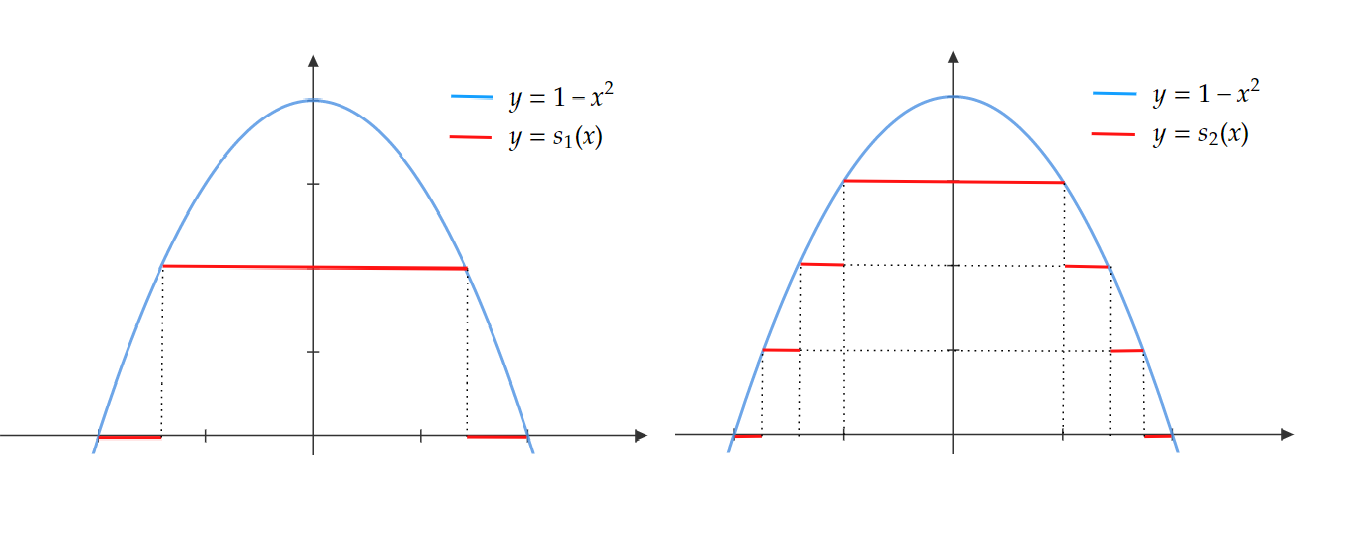
\includegraphics[height=6.4cm]{image/2.png}
    \caption{用简单函数逼近非负可测函数}
\end{figure}
% $\{a_1,a_2,\cdots,a_{m}\}$
\begin{theorem}\label{feifukecehanshukeyoujiandanhanshubijin}
    设$f:X\to [0,\infty]$是可测函数,那么存在渐升的非负简单可测函数列$\csf{s}\ (0\leq s_1\leq s_2\leq \cdots \leq f) $
    逐点收敛于$f$.\ $f$有界时,还可以要求一致收敛性。
\end{theorem}
\begin{proof}
        设$$s_n(x)=\left\{
            \begin{aligned}
                &\ \frac{k-1}{2^n}& \quad &\frac{k-1}{2^n}\leq f(x)<\frac{k}{2^n}\\
                &\ n &\quad &f(x)\geq n
            \end{aligned}
            \right.
            $$
        $s_n$是将f的值域划分成长度为$1/2^n$的若干个小区间,
        并在每个小区间取较小的那个值。 我们以函数$f(x)=1-x^2\ (x\in[-1,1])$为例,直观感受$s_n$是如何逼近f的(见上页图)。
\end{proof}
\ 


\begin{corollary}\label{jiandanhanshuyizhishoulianyukecehanshu}
    设$f$为可测函数,那么存在简单可测函数列$\csf{s}\ (\any i\in \ZZ_+,\ |s_i| \leq f) $收敛于$f$.\ $f$有界时,还可以要求一致收敛性。
\end{corollary}
\begin{proof}
    $f=f^+-f^-$,对$f$的正部和负部用简单函数分别逼近即可。
\end{proof}
\ 


在测度论中,我们称一个命题几乎处处为真,若这个命题在一个零测集以外处处为真。我们之后常说的几乎处处相等、几乎处处有限、几乎处处收敛等等,都是指在一个零测集之外满足该性质。
\begin{definition}\label{kecehanshushouliandemoshi} %可测函数收敛的模式
    设$(X,\Gamma,\mu)$为测度空间,$\kecef{f}$为可测函数列。
    \begin{enumerate}[(1)]
        \item 若$\any \ee>0,\ \mu(\{\limsup \limits_{n\to \infty}|f_n(x)-f(x)|>\ee\})=0$,称$f_n$\bi{几乎处处收敛}{jihuchuchushoulian}于$f$,记作$f_n\xrightarrow{a.e.}f$
        \item 若$\any \ee>0,\ \lim \limits_{n\to \infty}\mu(\{|f_n(x)-f(x)|>\ee\})=0$,称$f_n$\bi{依测度收敛}{yicedushoulian}于$f$,记作$f_n\xrightarrow{\mu}f$
        \item 若$\any \ee>0,\ \exi E\in \Gamma,\ \mu(E)<\ee$,在$X-E$中有$f_n\rightrightarrows f$,称$f_n$\bi{近一致收敛}{jinyizhishoulian}于$f$
    \end{enumerate}
\end{definition}

对几乎处处收敛,自然的定义方式是:$\exi$零测集$Z,\sothat \lim_{n\to \infty}f_n(x)= f(x),\ \any x \in X-Z$.\ 这
和定义\ref{kecehanshushouliandemoshi}(1)是等价的。事实上,这种定义方式等价于说
$\mu(\{\limsup_{n\to \infty}|f_n(x)-f(x)|>0\})\leq \mu(Z)=0$.\ 注意
$\mu(\{\limsup_{n\to \infty}|f_n(x)-f(x)|>0\})=\mu(\cu{k}\{\limsup_{n\to \infty}|f_n(x)-f(x)|>1/k\})$
在$\mu(\{\limsup_{n\to \infty}|f_n(x)-f(x)|>\ee\})$和$\cs{k}\mu(\{\limsup_{n\to \infty}|f_n(x)-f(x)|>1/k\})$之间,那么利用
夹逼容易证明两种定义方式等价。\\


对于上面的几种收敛模式,我们可以给出它们之间的关系。但是在这之前,我们必须讨论一个重要的问题:
可测函数列(几乎处处收敛)的极限是否依然是可测函数?答案是未必。设$f=g\ \ a.e.\ ,\ f$可测。设
零测集$E\in \Gamma$之外有$f=g$,\ 根据可测函数的定义,我们希望对任一开集$I\subseteq [-\infty,\infty]$,有$g^{-1}(I)$可测。
注意$g^{-1}(I)=\{x\in E\ :\ g(x)\in I\}\cup\{x\in E^c\ :\ g(x)\in I\}=(g^{-1}(I)\cap E)\cup(f^{-1}(I)\cap E)$,\ 
$f^{-1}(I)\cap E^c$为可测集,我们希望$g^{-1}(I)\cap E$作为零测集$E$的子集也可测。对于Lebesgue测度,这是显然的,因为所有零测集都可测。
但是对于一般的测度空间,这点不再成立。事实上,使得零测集的子集都可测的测度空间称为\bi{完备测度空间}{wanbeicedukongjian}。
\begin{definition}[测度空间的完备化]\label{cedukongjiandewanbeihua}\index{cedukongjiandewanbeihua@测度空间的完备化}
    设$(X,\Gamma,\mu)$为测度空间,记$\Gamma^*=\{E\subseteq X\ :\ \exi A,B\in \Gamma,\sothat A\subseteq E\subseteq B,\ \mu(B-A)=0\}$,那么$\Gamma^*$为一个$\sigma$-
    代数,对其中的元素定义其测度为$\mu(E)=\mu(A)=\mu(B)$,得到新的测度空间$(X,\Gamma^*,\mu)$.\ 这个过程称为测度空间的完备化。
\end{definition}
容易验证上述定义是良好的。并且,在此定义下,零测集的任一子集是零测集。在之后的讨论中,除非特别说明,我们都默认测度空间已经完备化。
事实上,我们定义的Lebesgue测度空间$(\RN,\mathfrak{M},m)$是Borel测度空间$(\RN,\mathfrak{B},m)$的完备化。根据定理\ref{lebesguekecejidekehua},对于任何一个Lebesgue可测集
$E$,存在$F_\sigma$集$H$(是Borel集)和$G_\delta$集$G$(是Borel集),使得$H\subseteq E\subseteq G,\ m(G-H)=0$.\ \\


下面我们给出几种收敛模式之间的关系。
\begin{theorem}\label{shoulianmoshizhijiandeguanxi} %收敛模式之间的关系
    设$(X,\Gamma,\mu)$为测度空间,$\kecef{f}$为几乎处处有限的可测函数列。
    \begin{enumerate}[(1)]
        \item 近一致收敛$\Rightarrow$依测度收敛、几乎处处收敛
        \item 依测度收敛$\Rightarrow$有子列近一致收敛$\Rightarrow$有子列几乎处处收敛
        \item 若$\mu(X)<\infty$,则几乎处处收敛$\Rightarrow$依测度收敛
        \item 若$\mu(X)<\infty$,则几乎处处收敛$\Rightarrow$近一致收敛
    \end{enumerate}
\end{theorem}
\begin{proof}
    \begin{enumerate}[(1)]
        \item 任给$\ee,\eta>0$,设在测度小于$\ee$的集合$E=E(\ee)$之外有$f_n\rightrightarrows f$.\ 那么存在$N=N(\eta,\ee)>0,\ \any n\geq N,\ x\in X-E,\ |f_n(x)-f(x)|<\eta$,故
$$\mu(\{|f_n(x)-f(x)|>\eta\})\leq \mu({E})<\ee,$$由$\ee$的任意性可知$f_n$依测度收敛;由于在$X-E$内有$\lim_{n\to \infty}|f_n-f|=0$,故
        $$\mu(\lim_{n\to \infty}\{|f_n(x)-f(x)|>\eta\})\leq \mu({E})<\ee,$$由$\ee$的任意性可知$f_n$几乎处处收敛。
        \item 设$f_n\xrightarrow{\mu}f$,那么对任意正数m,数列$a_n=\mu(|f_n(x)-f(x)|>1/m)$收敛到0,故存在$n_m\in \ZZ_+$使得$a_{n_m}<1/2^m$.\ 
        对于函数列$\{f_{n_m}\}_{m=1}^{\infty}$,由于$$\cs{m}\mu(\{|f_{n_m}(x)-f(x)|>1/m\})<1,$$那么任给$\ee>0$,存在$N=N(\ee)$,
        $$\ee>\sum_{m=N}^{\infty}\mu(\{|f_{n_m}(x)-f(x)|>1/m\})\geq \mu(\cup_{m=N}^{\infty}\{|f_{n_m}(x)-f(x)|>1/m\}).$$设$E=\cup_{m=N}^{\infty}\{|f_{n_m}(x)-f(x)|>1/m\}$,故在E之外
        总有$|f_{n_m}(x)-f(x)|\leq 1/m\to 0\ \ (m\to \infty)$,在$X-E$上$f_{n_m}$一致收敛,故$f_{n_m}$近一致收敛。根据(1),$f_{n_m}$几乎处处收敛。
        \item 设$f_n \xrightarrow{a.e.} f$,则$\any \ee>0,\ 0=\mu(\{\limsup_{n\to \infty}|f_n(x)-f(x)|>\ee\})=$
        $\mu(\limsup_{n\to \infty}\{|f_n(x)-f(x)|>\ee\})$(这一步利用数列、集合列的上极限定义不难证明)
        $=\mu(\lim_{k\to \infty}\cup_{n=k}^{\infty}\{|f_n(x)-f(x)|>\ee\})=\lim_{k\to \infty}\mu(\cup_{n=k}^{\infty}\{|f_n(x)-f(x)|>\ee\})$(这一步用到了X的测度小于无穷,以及测度的从上连续性)
        $\geq \lim_{k\to \infty}\mu(\{|f_k(x)-f(x)|>\ee\})$,得到依测度收敛性。
        \item 这个证明略需技巧。考虑$g_n=\sup_{k\geq n}|f_k-f|$,注意$$f_n\rightrightarrows f \Longleftrightarrow \exi \{n_k\}_{k=1}^{\infty}\subseteq \ZZ_+,\ g_{n_k}\rightrightarrows 0,$$而我们已知
        $0\leq g_n\leq |f_n-f|\xrightarrow{a.e.}0$,那么根据(3),$g_n$依测度收敛,再根据(2),它有子列近一致收敛,从而易见$f_n$近一致收敛。
    \end{enumerate}
\end{proof}
\ 


\begin{note}
    与概率论中不同,几乎处处收敛并不强于依测度收敛(反之亦然)。反例如下:
\end{note}
\ 


\begin{example}
    设$(\RR,\mathfrak{M},m)$为Lebesgue测度空间,$f_n=\chi_{[n-1,n]},\ g_n=\chi_{[j/2^k,(j+1)/2^k]},\ n=2^k+j,\ 0\leq j <2^k$.\ 
    那么$f_n\xrightarrow{a.e.} 0,\ g_n\xrightarrow{m}0$,但$f_n$不依测度收敛,$g_n$不几乎处处收敛。
\end{example}
\ 

\begin{proposition}
    函数列$f_n$依测度收敛当且仅当它是依测度Cauchy列。
\end{proposition}
\begin{proof}
必要性:$f_n\xrightarrow{\mu} f$ 当且仅当对于任意 \(\epsilon,\eta > 0\),存在 $N>0$ 使得 $$
\forall \,n>N,\,\mu(E_\epsilon^n)<\eta,\,\,E_\epsilon^n:=\{x\in X\,:\,|f_n(x)-f(x)|\geq \epsilon  \},
$$ 注意到任给 $m,n>N,\,x\in (E_\epsilon^n\cup E_\epsilon^m)^c$ 时 $$|f_n(x)-f_m(x)|\leq |f_n(x)-f(x)|+|f(x)-f_m(x)|<2 \epsilon ,$$ 这说明 $\exists\,N>0,\,\forall\,n,m >N$,\[
\mu(\{x \in X :|f_n(x) - f_m(x)| \geq 2\epsilon\}) \leq \mu(E_\epsilon^n\cup E_\epsilon^m)<2\eta
\]  这说明 $(f_n)$ 是依测度Cauchy列。


充分性  :
若 \((f_n)\) 是依测度Cauchy列,则对于任意 \(\epsilon,\,\delta > 0\),存在 \(N(\delta,\epsilon)>0\),使得当 \(n, m > N\) 时,   \[
\mu(E_{\epsilon}^{m,n}) < \delta,\,E_\epsilon^{m,n}:=\{x \in X : |f_n(x) - f_m(x)| \geq \epsilon\},
\] 我们通过如下方式构造 $(f_n)$ 的依测度极限函数(之后验证合理性):$$
f=f_{a_1}+\sum_{n=1}^{\infty} (f_{a_{n+1}}-f_{a_{n}} ),
$$ 其中 $a_n$ 是单增趋于无穷的正整数序列,且 $$\mu(E_{2^{-n}}^{a_n,a_{n+1}})<2^{-n},\,E_{2^{-n}}^{a_n,a_{n+1}}:=\{x\in X\,:\, |f_{a_n}(x)-f_{a_{n+1}}(x)|\geq 2^{-n} \}.$$ 易见$\sum_{n=1}^{\infty}\mu( E_{2^{-n}}^{a_n,a_{n+1}}  )\leq 1$,这说明 $\mu(\limsup_{n  \to \infty} E_{2^{-n}}^{a_n,a_{n+1}})=0 $,并且在 $\limsup_{n  \to \infty} E_{2^{-n}}^{a_n,a_{n+1}}$ 的补集上,成立 $$
\exists\, N>0,\,\forall\,n>N,\,x\notin  E_{2^{-n}}^{a_n,a_{n+1}},\,\,i.e.\,\,|f_{a_n}(x)-f_{a_{n+1}}(x)|< 2^{-n}.
$$ 这说明在 $\limsup_{n  \to \infty} E_{2^{-n}}^{a_n,a_{n+1}}$ 的补集上,$\sum_{n=t}^{\infty}|f_{a_{n+1}}-f_{a_n}|\leq 2^{-l+1} $,即 $f$ 的定义式绝对收敛。这说明 $f$ 的定义是一个几乎处处收敛的定义。

下面证明 $f_n \xrightarrow{\mu} f$. 事实上,任给 $\epsilon,\,\eta>0$,设 $2^{-l+1}<\epsilon$,则 $$
|f_n-f|\leq |f_{a_{l}}-f_n|+\sum_{n=t}^{\infty}|f_{a_{n+1}}-f_{a_n}|\leq |f_{a_{l}}-f|+ 2^{-l+1} \leq |f_{a_{l}}-f_n|+\epsilon,
$$ 由依测度Cauchy列的定义,存在 $M,\,l,n>M$ 时,成立 $$
\mu(\{x\in X\,:\, |f_n(x)-f(x)|\geq 2\epsilon\})=\mu(E_{2\epsilon}^n)\leq \mu(E_{\epsilon}^{n,a_l})\leq \eta.
$$ 这就说明了 $f_n \xrightarrow{\mu} f$. 
\end{proof}
\,


下面的定理告诉我们,几乎处处有限的可测函数与连续函数相差很小(在一个测度任意小的集合外就是连续函数)。但是一般来说不能称可测函数是几乎处处连续的,
反例见例\refp{kecehanshubujihuchuchulianxu}。

\begin{theorem}[Lusin]\label{lusindingli}\index{lusindingli@Lusin定理}
    设$E\subseteq \RN$为可测集,$f:E\to [-\infty,\infty]$是几乎处处有限的可测函数,那么任给$\delta>0$,存在闭集$F\subseteq E,\ m(E-F)<\delta$,使得
    $f\in C(F)$(即$f$在$F$上连续)。
\end{theorem}
\begin{proof}
    不妨设$f$为有界函数(不然,设$g(x)=\frac{f(x)}{1+|f(x)|}$,不难说明$f(x)=\frac{g(x)}{1-|g(x)|}$,$f$连续当且仅当$g$连续,用$g$代替$f$进行讨论即可)。
    注意$|g|< 1$,由推论\ref{jiandanhanshuyizhishoulianyukecehanshu}知存在可测简单函数列$\{\varphi_n(x)\}_{n\in \ZZ_+}$
    在$E$上一致收敛于$g(x)$,我们下面只用考虑简单函数的情况。我们希望构造一个闭集$F$,
    使得在$F$上简单函数列$\{\varphi_n(x)\}_{n\in \ZZ_+}$连续,从而一致收敛于连续函数。


    一般地,设$\jd{s}$为简单函数,其中$A_i$都是包含在$E$中的不交可测集,其并集为$E$.\ 任给$\eta>0$,根据可测集的性质,存在闭集$F_i\subseteq A_i$,使得
    $m(A_i-F_i)<\eta/n$,取$F_0=\cup_{i=1}^{n}F_i$,则在$F_0$上$s$为连续函数(不难直观感受,也可以由下面的
    粘接引理得到),且$m(E-F_0)<\eta$。对于每个简单函数$\varphi_n$,我们选取对应的闭集$F_0^{(n)}\subseteq E,\ m(E-F_0^{(n)})<\delta/2^n$,
    使得$\varphi_n$在其中连续。令$F=\ci{n}F_0^{(n)}$,则$m(E-F)\leq \cs{n}m(E-F_0^{(n)})<\delta$,易见$F$上$\varphi_n $一致收敛于$f$,故
    $f\in C(F)$.
\end{proof}
\


\begin{lemma}[粘接引理]\label{zhanjieyinli}\index{zhanjieyinli@粘接引理}
    设$\{F_1,\cdots,F_n\}$为X的有限闭覆盖,且映射$f:X\to Y$在每个$F_i$的限制上都连续,那么$f$为X上的连续映射。
\end{lemma}
\begin{proof}
    设F为Y中闭集。我们证明$f^{-1}(F)$为闭集,从而$f$为连续映射。注意$f^{-1}(F)=\cup_{i=1}^{n}(f^{-1}(F)\cap F_i)$,$f^{-1}(F)\cap F_i=f^{-1}_{F_i}(F)$为$F_i$中闭集,故
    也是X中闭集。$f^{-1}(F)$为有限个闭集的并集,故也是闭集。
\end{proof}
\ 


在定理\ref{lusindingli}中,所得到的$F$上的连续函数$f$可以扩张到$E$上,并且上确界不超过$f$在$F$中的上确界。
上述结论需要拓扑学中的Tietze扩张定理,这里仅作介绍,证明不涉及实变函数的核心内容,故略去:
\begin{theorem}[Tietze扩张定理]\label{tietzekuozhangdingli}
    设$X$为$T_4$拓扑空间,即$X$中任意一个包含于开集$E$的闭集$F$,存在开集$U,\ F\subseteq U \subseteq E,\sothat \overline{U}\subseteq E$,那么$F$上的连续函数
    可以扩张到$X$上,并且上确界不超过在$F$中的上确界。
\end{theorem}

$\RN$是度量空间,从而是$T_4$的,满足定理适用条件。现在我们设扩张得到的连续函数是$g(x)$,如果我们设$E$为有界集(设$E\subset B(0,k)$),还可以要求$g$具有紧支集
(函数$f:X\to \RR$的\bi{支集}{zhiji}是指$\textrm{supp}(f):=\overline{\{x\in X\ :\ f(x)\neq 0\}}$,其中上划线表示闭包)。
事实上,设\begin{equation*}
    \varphi(x)=\frac{d(x,(B(0,k))^c)}{d(x,(B(0,k))^c)+d(x,F)}
\end{equation*}
$\varphi(x)$为连续函数,将上述$g(x)$换为$\varphi(x)g(x)$即可。
\\


由上面的讨论不难得出下面命题:
\begin{proposition}\label{jinzhijilianxuhanshubijinkecehanshu}
    设$m(E)<\infty$,$f:E\to [-\infty,\infty]$是几乎处处有限的可测函数,则
    $\any \delta>0$,存在$\RN$上有紧支集的连续函数$g$,使得$f,g$不相等的点集测度小于$\delta$,并且$g$的上确界不超过$f$的上确界。
\end{proposition}
% \begin{proof}
%     1\\2\\留白
% \end{proof}
% \ 

最后我们指出,若$f(x)$为$E\subseteq \RN$上几乎处处有限的可测函数,
那么存在$\RN$上的连续函数列$\csf{g},\sothat$ 在E中$g_k(x)\xrightarrow{a.e.}f(x)$.\ 
这是因为:$\any \ee>0,\ \any n\in \ZZ_+,\ \exi g_n\in C(\RR),\sothat m(\{|f(x)-g_n(x)|>\ee\})<1/n$. 这说明
$g_n\xrightarrow{m}f$,故存在子列几乎处处收敛到$f$.\\
\ 

%%%%%%%%%%%%%%%%%%%%%%%%%%%%%%%%%%%%%%%%%%%%%%%%%%%
\newpage\section{Cantor集与Cantor函数}
下面我们要介绍的Cantor集与Cantor函数为我们提供了丰富的反例。


我们首先归纳地定义Cantor集。首先固定$d\in (0,1/3]$.\ 设$E_0=[0,1]$,在$E_0$的中心挖去长度为
$d$的一个开区间$J_1$,得到的集合设为$E_1$,它是两个闭区间$[0,(1-d)/2],\ [(1+d)/2,1]$的并集。在每个闭区间的中心
挖去长度为$d^2$的开区间$J_{2,1},\ J_{2,2}$,得到的集合设为$E_2$,它是四个闭区间的并集。依此类推,
在第n步,我们得到$E_n$,它是$2^n$个闭区间的并集,这一步挖去的开区间是$J_{n,1},\cdots,J_{n,2^{n-1}}$,\ 
长度均为$d^n$.\ 我们设$J_n=\cup_{k=1}^{2^{n-1}}J_{n,k},\ m(J_n)=(2d)^n/2,\ m(\cu{n}J_n)=\cs{n}m(J_n)=d/(1-2d)$.\ 
定义\bi{类Cantor集}{leicantorji}为$C_d:=\ci{n}E_n=E_0-\cu{n}J_n$,\ 它是可测集,测度是$1-m(\cu{n}J_n)=(1-3d)/(1-2d)\in[0,1)$.\ 
\begin{definition}[Cantor集]\label{cantorjidingyi}
    在类Cantor集$C_d$中取$d=1/3$,得到的集合称为\bi{Cantor集}{cantorji},记为C.\ 
\end{definition}
\begin{wrapfigure}{r}{0pt}
    \centering
    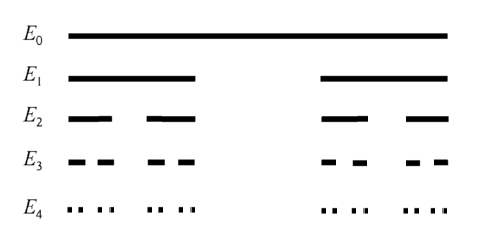
\includegraphics[height=4cm]{image/3.jpeg}
    \caption{Cantor集的构造}
\end{wrapfigure}
根据定义,$C_d$是若干闭集的交集,故为$\RR$中的有界闭集,进而是紧集;同时容易看出$C_d$没有内点。


我们把集合E的所有聚点构成的集合称为E的导集,记为$E^{'}$.\ 如果$E=E^{'}$,就说E是\bi{完全集}{wanquanji}。容易看出完全集没有孤立点。
$C_d$为完全集。由于$C_d$为闭集,故$C_d^{'}\subseteq C_d$,我们只需要证明$C_d \subseteq C_d^{'}$.\ 任给$x\in C_d$,我们要说明$\any \delta>0,\ ((x-\delta,x)\cup(x,x+\delta))\cap C_d \ne \emptyset $.\ 根据定义,有
$\any n\in\ZZ_+ ,\ x\in E_n$,设当$n$足够大时,构成$E_n$的闭区间长度足够小,以至于端点落在了$(x-\delta,x)\cup(x,x+\delta)$中。注意区间端点是
属于$C_d$的,从而$((x-\delta,x)\cup(x,x+\delta))\cap C_d \ne \emptyset $.\ 


此外,$C_d$还是不可数集。当$d<1/3$,$m(C_d)>0$,当然$C_d$是不可数集。下面我们只考虑$C_{1/3}=C$的情况。这就是我们前面提到的反例:
\\ \ 
\begin{example}\label{ceduweilingdebukeshudianji}
    存在测度为0的不可数点集(取Cantor集C即可)。
\end{example}
\begin{proof}
    根据前面的讨论,C为零测集。下面说明C不可数。我们说明C中数的三进制表示一定形如$0.a_1a_2\cdots a_n\cdots,\ a_i=0,2$(即$C=\{\cs{i}a_i/3^i\ :\ a_i=0,2\}$)即可。
    我们考虑去掉的开区间  $J=\cu{n}J_n$,只需说明去掉的开区间中的数的三进制表示一定不为上述形式。
    断言:$x\in J_{n,k} \Longleftrightarrow x=0.a_1a_2\cdots a_{n-1}1\ a_{n+1}\cdots$,其中$a_1,\cdots,a_{n-1}\in \{0,2\}$,$a_{n+1},a_{n+2},\cdots$
    不全为0(否则为区间左端点),也不全为2(否则为区间右端点)。断言的证明是简单的归纳,这里略去。
\end{proof}
\ 


根据前面的讨论,$C=\{\cs{i}a_i/3^i\ :\ a_i=0,2\}$,我们据此定义Cantor函数。
对于$x=\cs{i}a_i/3^i\in C\ (a_i=0,2)$,设$f:C\to [0,1],\ x\mapsto \ \cs{i}\frac{1}{2}\cdot \frac{a_i}{2^{i}}$,那么$f$为不严格单增的满射,但不是单射
(容易验证$f(1/3)=f(2/3)=0.5$,事实上在挖掉的区间端点处$f$取值相同)。
\begin{definition}[Cantor函数]\label{cantorhanshudingyi}
    设$g:[0,1]\to [0,1],\ x\mapsto \sup\{f(y)\ :\ y\leq x,\ y\in C\}$,其中$f:C\to [0,1],\ \cs{i}\frac{a_i}{3^i}\mapsto \cs{i}\frac{a_i}{2^{i+1}}$.\ 我们称$g$为\bi{Cantor函数}{cantorhanshu}。
\end{definition}

容易看出$g$单增且是满射,但不是单射,它在去掉的每个开区间内取值为常数。
\ \\
\begin{example}\label{daoshujihuchuchuweilingdanbushichangshu}
    几乎处处可导且导数为0的函数不一定为常数。
\end{example}
\begin{proof}
    Cantor函数$g$在去掉的每个开区间内取值为常数,从而导数为0;由于去掉的区间测度和为1,因此Cantor函数几乎处处可导且导数为0,但它不是常数。
\end{proof}
\ 


\begin{proposition}
    Cantor函数$g$是单增连续满射,并且具有对称性:$g(x)+g(1-x)=1$.\ 
\end{proposition}
\begin{proof}
    显然$g$为单增满射,如果它在$x_0\in [0,1]$不连续,因其单增性,间断点必为跳跃间断点,故不可能形成到$[0,1]$的满射,从而$g$连续。

    另一方面,由于$C=\{\cs{i}a^i/3^i\ :\ a_i=0,2\}$,若$x\in C$,可设$x=\cs{i}x_i/3^i$,则$1-x=\cs{i}(2-x_i)/3^i\in C$.\ 那么
    $g(x)+g(1-x)=f(x)+f(1-x)=\cs{i}x_i/2^{i+1}+\cs{i}(2-x_i)/2^{i+1}=1$.\ 若$x\notin C$,设$x_1=\sup\{y\in C\ :\ y\leq x\}$,
    $x_2=\inf\{y\in C\ :\ y\geq x\}$,$x_1,x_2$是某个被挖去的小区间的端点,设\begin{equation*}
        x_1=0.z_1z_2\cdots z_k0222\cdots,\ x_2=0.z_1z_2\cdots z_k2222\cdots,\ x=z_1z_2\cdots z_k1z_{k+2}\cdots,
    \end{equation*}
    其中$z_i\ (i\geq k+2)$不全为2、不全为0.\  
    设$\tilde{x}=1-x,\ \tilde{z_i}=2-z_i$.\ 则\begin{equation*}
        \tilde{x}=\tilde{z}_1\tilde{z}_2\cdots \tilde{z}_k1\tilde{z}_{k+2}\cdots,\ \ \sup\{y\in C\ :\ y\leq \tilde{x}\}=\tilde{z}_1\tilde{z}_2\cdots \tilde{z}_k0222\cdots=1-x_2.
    \end{equation*}
    那么$g(x)+g(1-x)=f(x_1)+f(1-x_2)=f(x_2)+f(1-x_2)=1$.\ 
\end{proof}
\ 


\begin{example}\label{lingcejidexiangbulingce}
    连续的一一对应未必将零测集映为零测集。    
\end{example}
\begin{proof}
    令$g$为Cantor函数,$\psi(x)=\frac{x+g(x)}{2}$,这是一个严格单增、连续的、$[0,1]\to [0,1]$的一一对应。设Cantor集中第n步挖去的
    开区间为$\{J_{n,k}\}_{k=1}^{2^{n-1}}$,注意$g$在挖掉的开区间内为常数,那么$\psi(I_{n,k})$为长度为$|I_{n,k}|/2$的开区间。
    设$J=\cu{n}\cup_{k=1}^{2^{n-1}}J_{n,k}$,那么$m(\psi(J))=1/2,\ m(\psi(C))=m(\psi([0,1]-J))=m(\psi([0,1])-\psi(J))=1/2$.\ 
    C是零测集,但$\psi(C)$测度为正。
\end{proof}
\ 


$\RR$中全体可测集构成的集合$\mathfrak{M}$的势为$\aleph_2$:考虑Cantor集C的全体子集,它们都是零测集,进而可测,故$\textrm{card}(\mathfrak{M})\geq \textrm{card}(2^C)=\textrm{card}(2^\RR)=2^{\aleph_1}=\aleph_2$.\ 
另一方面,$\textrm{card}(\mathfrak{M})\leq \textrm{card}(2^\RR)=\aleph_2$,得到$\textrm{card}(\mathfrak{M})=\aleph_2$
(此外,任一可测集与不可测集的无交并不可测,易见不可测集全体的势也是$\aleph_2$)。
另一方面,Borel代数的势为$\aleph_1$(证明需要超限归纳法,此处略去),故存在不是Borel集的可测集。
事实上,我们也可以直接构造不是Borel集的可测集:\\


\begin{example}\label{feiboreljidekeceji}
    存在不是Borel集的可测集(零测集)。
\end{example}
\begin{proof}
    我们沿用例\ref{lingcejidexiangbulingce}的记号。
    根据定理\ref{steinhuasdingli},$\psi(C)$存在不可测子集$W$,记$\psi^{-1}(W)=S\subset C$,则S为零测集(故可测)。但是S不是Borel集,否则根据
    命题\ref{boreljideyuanxiang}不难说明:对于一一对应的一元连续函数,其反函数连续,故Borel集的像是Borel集,从而W是Borel集,与W不可测矛盾。
\end{proof}
\


\begin{remark}
    我们还同时说明了,连续函数未必将可测集映为可测集。这里的S是零测集,但它的像不可测。之后我们将说明,绝对连续函数将零测集映为零测集、将测度小于无穷的可测集映为可测集。
\end{remark}
\ 


设$C_{d}$为类Cantor集,构造过程中挖掉的可数个开区间记为$\{I_{j}\}_{j=1}^{\infty}$。设I为$[0,1]$中任意一个开区间,如果I与$C_{d}$相交,
I必然包含上述某个$I_{j}$(注意每步挖掉开区间后,得到的若干闭区间长度是趋于0的,故若I与$C_{d}$相交,I必然包含某一步所得到的闭区间,在下一步时,这个闭区间中心的开区间会被挖去),
从而总有$m(I\cap C_{d})<m(I)$。注意到这点,我们可以提供下面的例子。这个例子表明,存在一个正测度可测集E,它在任何一个区间内的密度严格大于0小于1。\\
\begin{example}\label{zhengcedujibuwanquanbaohanjuti}
    存在正测度可测集$E$,使得对任意一个矩体$I$,有$0<m(I\cap E)<m(I)$.\ (或等价地表述为:存在正测度可测集$E$,
    使得对任意一个矩体$I$,有$m(I\cap E)>0,\ m(I\cap E^c)>0$.)
\end{example}
\begin{proof}
    我们在[0,1]中考虑该命题,矩体就是区间。
    首先,考虑类Cantor集$H_1=C_{d_1}\ \sothat m(C_{d_1})=1/2$,设构造过程中挖掉的可数个开区间为$\{I_{1,j}\}_{j=1}^{\infty}$。我们对挖去的每个开区间$I_{1,j}$,类似于之前在$[0,1]$
    中的作法,作类Cantor集$C_{d_2}\ \sothat m(C_{d_2})=|I_{1,j}|/2^2$(得到的所有类Cantor集$C_{d_2}$的并集记为$H_2$),再设构造过程中挖掉的所有开区间为$\{I_{2,j}\}_{j=1}^{\infty}$,对每个开区间,再作类Cantor集$C_{d_3}\ \sothat m(C_{d_3})=|I_{2,j}|/2^3$,依次类推。
    设$E=\cu{n}H_n$,易见E为可测集。


    设I为$[0,1]$中任意一个开区间,易见在上面的构造方法下,I必与某个类Cantor集相交,根据上面的讨论,它必然包含某个挖去的开区间,记为$I_{s,t}$.\ 
    我们在这个挖去的开区间中构造新的类Cantor集,
    总的测度为$c\cdot |I_{s,t}|,\ c=c(s)\in(0,1)$,那么$m(I)-m(I\cap E)=m(I\cap E^c)\geq |I_{s,t}|\cdot (1-c)>0$.\ 
    另一方面,$m(I\cap E)\geq |I_{s,t}|\cdot c>0$,故$0<m(I\cap E)<m(I)$.\ 
\end{proof}
\ 


\begin{example}\label{kecehanshubujihuchuchulianxu}
    可测函数未必几乎处处连续。
\end{example}
\begin{proof}
    考虑类Cantor集$C_{1/4}$,设$$f(x)=\left\{
        \begin{aligned}
            &1&\quad&x\in C_{1/4}\\
            &-1&\quad&x\in [0,1]-C_{1/4}
        \end{aligned}
    \right. $$
    那么$f$可测,但是任给零测集Z,总有$C_{1/4}-Z=([0,1]-Z)\cap C_{1/4}$非空,
    设$x\in ([0,1]-Z)\cap C_{1/4}$,任给$\delta>0,\ $根据之前的讨论,$(x-\delta,x+\delta)$中必然含有某个被挖去的开区间,故也含$[0,1]-C_{1/4}-Z$中的点,故
    $f$(作为$[0,1]-Z$上的函数)不在$x$处连续,从而$f$不在任一零测集之外连续。
\end{proof}
\ 




%%%%%%%%%%%%%%%%%%%%%%%%%%%%%%%%%%%%%%%%%%%%%%%%%%%
%%%%%%%%%%%%%%%%%%%%%%%%%%%%%%%%%%%%%%%%%%%%%%%%%%%
%%%%%%%%%%%%%%%%%%%%%%%%%%%%%%%%%%%%%%%%%%%%%%%%%%%
\chapter{Lebesgue积分}
\section{可测函数的积分}
对于测度空间$(X,\Gamma,\mu),$设$\jd{s}$,在没有特殊说明的情况下,我们都认为$s$是$X\to [0,\infty]$的非负可测简单函数,
其中$a_i\geq 0,\ A_i=s^{-1}(a_i)$互不相交。
\begin{definition}
    设$(X,\Gamma,\mu)$为测度空间,$\jd{s}$为非负可测简单函数,定义$s$在$E\in \Gamma$上的积分为:
    \begin{equation*}
        \int_{E}s \ d\mu := \sum_{i=1}^{n}a_i\mu(A_i\cap E)=\int_{X} s\cdot \chi_{E}\ d\mu
    \end{equation*}
    设$\ff{f}$为非负可测函数,定义$f$在$E\in \Gamma$上的积分为:
    \begin{equation*}
        \int_{E}f \ d\mu:= \sup_{0\leq s\leq f} \int_{E}s \ d\mu\ (\ff{s}\mbox{为简单可测函数})
    \end{equation*}
    设$f$为一般的可测函数,若$\int_{E}f^+\ d\mu,\ \int_{E}f^-\ d\mu$不全为无穷(否则称$f$的积分不可定义),那么定义$f$在$E\in \Gamma$上的积分为
    \begin{equation*}
        \int_{E}f \ d\mu:= \int_{E}f^+ \ d\mu-\int_{E}f^- \ d\mu
    \end{equation*}
    当测度空间取$(\RN,\mathfrak{M},m)$时,上述积分称为\bi{Lebesgue积分}{lebesguejifen}。
\end{definition}
根据定义不难验证下面的命题:
\begin{proposition}\label{jifenxingzhi}
    设$(X,\Gamma,\mu)$为测度空间,$E,F\in \Gamma$,$f,g$为可测函数。则:
    \begin{enumerate}[(1)]
        \item 若$0\leq f\leq g$,则$\int_{E}f \ d\mu\leq \int_{E}g \ d\mu$
        \item 若$E\subseteq F,\ f\geq 0$,则$\int_{E}f \ d\mu \leq \int_{F}f\ d\mu$
        \item 对实数c,$\int_{E}cf \ d\mu =c\int_{E}f \ d\mu $
        \item 若$f(x)=0\ \ a.e.\ $,则$\int_{E}f\ d\mu=0$
        \item 若$\mu(E)=0,\ \int_{E}f\ d\mu=0$
        \item 对$E\subseteq X$,有$\int_{E}f\ d\mu=\int_{X}f\chi_{E}\ d\mu$
    \end{enumerate}
\end{proposition}
对最后一条我们简单证明。不妨设$f$非负,首先,$\int_{X}f\chi_{E}\ d\mu=\ffint{f\chi_{E}}$,由于$s$在E之外取值为0,
故$\int_{X}f\chi_{E}\ d\mu = \sup_{0\leq s\leq f\chi_{E}}\sum_{A_i\subseteq E}a_i\mu(A_i\cap E)\leq \sup_{0\leq s\leq f}\sum_{i=1}^{n}a_i\mu(A_i\cap E)=\int_{E}f\ d\mu$.\ 
此外,$\int_{E}f\ d\mu=\ffinte{f}=\sup_{0\leq s\leq f}\int_{X}s\chi_{E}\ d\mu\leq \int_Xf\chi_{E}\ d\mu$.\ 综上所述就证明了命题。\\


在下面的表达式中,不加说明时,我们是在可测空间$(X,\Gamma,\mu)$中考虑问题。有时我们省略积分中的$d\mu$;
如果集合列$\csf{E}$两两不交,其并集可以写为$\cs{k}E_k$,我们在采用这种记号时也默认$\csf{E}$为两两不交的集合列。


下面这个命题根据定义不难验证,故略去证明。
\begin{proposition}\label{phishizhengcedu}
    设$\jd{s}$为非负简单可测函数(对一般的非负可测函数,我们在命题\ref{phishizhengcedu2}中讨论),那么$\varphi:\Gamma\to [0,\infty],\ E\mapsto \int_{E}s\ d\mu$为正测度。即:
    $\int_{\emptyset}s\ d\mu=0,\ \int_{\cs{n}E_n}s\ d\mu=\cs{n}\int_{E_n}s\ d\mu$,其中$\csf{E}$为不交可测集列。
\end{proposition}

结合这个命题,并根据正测度的性质,我们还可以得到:
    \begin{itemize}
        \item $\int_{\sum_{i=1}^{n}E_i}s\ d\mu=\sum_{i=1}^{n}\int_{E_i}s\ d\mu$(并集写成求和记号时,默认集合两两不交);
        \item 对单增集合列$\csf{E}$,有$\lim_{k\to \infty}\int_{E_k}s \ d\mu=\int_{\lim_{k\to \infty}E_k}s \ d\mu$;
        \item 对于测度小于无穷的单减集合列$\csf{E}$,上个结论也成立。
    \end{itemize}
\,


值得说明的是,积分的线性性质并不是一件显然的事情。对于非负简单可测函数,我们指出:有限个函数积分的和等于它们的和的积分。以两个函数为例,
$\jd{s},\ t=\sum_{j=1}^{m}b_j\chi_{B_j}$,\ 那么易见$s+t=\sum_{i=1}^{n}\sum_{j=1}^{m}(a_i+b_j)\chi_{A_i\cap B_j}$.\ 
在每个$E_{i,j}=A_i\cap B_j$上,有$\int_{E_{i,j}}s+t=(a_i+b_j)\mu(E_{i,j})=\int_{E_{i,j}}s+\int_{E_{i,j}}t$,再利用命题\ref{phishizhengcedu},
考虑正测度的有限可加性,就得到欲证结论。但对一般的可测函数,我们暂时还不清楚积分的线性性质,其证明需要更多的结论。
下面的结论被称为单调收敛定理\index{dandiaoshouliandingli@单调收敛定理}:

\begin{proposition}[Beppo Levi]\label{dandiaoshouliandingli}\index{beppolevidingli@Beppo Levi定理}
    设$\csf{f}$为非负单增可测函数列,设$\lim_{n\to \infty}f_n(x)=f(x)$,那么$f$为非负可测函数,并且
    \begin{equation*}
        \lim_{n\to \infty}\int_{X}f_n=\int_{X}\lim_{n\to \infty}f_n=\int_{X}f
    \end{equation*}
\end{proposition}
\begin{proof}
    由于$f_n\leq f$,故$\lim_{n\to \infty}\int_{X}f_n\leq \int_{X}\lim_{n\to \infty}f_n$.\ 
    任意给定$s:X\to [0,\infty],s\leq f$,其中s为简单可测函数,设$E_n=\{x\in X\ :\ f_n(x)\geq c\cdot s(x)\}$,其中c为任意给定的严格位于0和1之间的实数。
    易见$E_n$可测,并且单增地趋于X.\ 于是有
    $\int_{X}f_n\geq \int_{E_n}f_n\geq \int_{E_n}c\cdot s$,令$n\to \infty$,根据命题\ref{phishizhengcedu}得:
    \begin{equation*}
        \lim_{n\to \infty}\int_{X}f_n\geq \lim_{n\to \infty}\int_{E_n}c\cdot s=\int_{\lim_{n\to \infty} E_n}c\cdot s=c\cdot \int_{X}s.
    \end{equation*}
    令c趋于1,根据s的任意性,我们得到$\lim_{n\to \infty}\int_{X}f_n\geq \int_{X}\lim_{n\to \infty}f_n$,这就完成了证明。
\end{proof}
\ 


根据单调收敛定理,我们可以说明对非负可测函数,积分有线性性质。事实上,设$s_n$单增趋于$f$,$\widetilde{s_n}$单增趋于$g$,那么
$\int_{X}f+g=\int_{X}\lim_{n\to \infty}s_n+\widetilde{s_n}=\lim_{n\to \infty}\int_{X}s_n+\widetilde{s_n}=$
$\lim_{n\to \infty}\int_{X}s_n+\lim_{n\to \infty}\int_{X}\widetilde{s_n}=\int_{X}\lim_{n\to \infty}s_n+\int_{X}\lim_{n\to \infty}\widetilde{s_n}=\int_Xf+\int_Xg$
(对于减法同理成立)。
对于一般的可测函数,积分也有线性性质,考虑其正部、负部即可。其证明思路是容易的,但表达较为繁琐,在此略去。


在Riemann积分中,我们未必有可数个非负函数和的积分等于积分的和(一般要求一致收敛性,或者在闭区间收敛于连续函数(Dini定理))。但是在Lebesgue积分中,
这点不再需要保证。
\begin{proposition}\label{jifendehedengyuhedejifen}
    设$\ff{f_n}$可测,则$\int_X \cs{n}f_n=\cs{n}\int_{X}f_n$.\ 
\end{proposition}
\begin{proof}
    设$g_N=\sum_{i=1}^{N}f_i$,则$g_N$单增趋于$f$,由单调收敛定理和积分的线性性质易得结论。
\end{proof}
\ 


\begin{lemma}[Fatou]\label{fatouyinli}\index{fatouyinli@Fatou引理}
    设$\ff{f_n}$可测,则$\int_{X}\linf{f}\leq \liminf_{k\to \infty}\int_Xf_k$.\ 
\end{lemma}
\begin{proof}
    设$g_n=\inf_{k\geq n}f_k$,$g_n$单增趋于$\linf{f}$.\ 那么$\int_{X}\linf{f}=\lim_{n\to \infty}\int_{X}\inf_{k\geq n}f_k=$
    $\liminf_{n\to \infty}\int_{X}\inf_{k\geq n}f_k\leq \liminf_{n\to \infty}\int_{X}f_n$.\ 
\end{proof}
\ 


下面这个命题是命题\ref{phishizhengcedu}的加强。
\begin{proposition}\label{phishizhengcedu2}
    设$\ff{f}$为非负可测函数,那么$\varphi:\Gamma\to [0,\infty],\ E\mapsto \int_{E}f\ d\mu$为正测度,并且
    \begin{equation*}
        \any \ff{g} \mbox{可测,}\int_{X}g\ d\varphi=\int_Xgf\ d\mu
    \end{equation*}
\end{proposition}
\begin{proof}
    先证明$\varphi$为正测度。我们只证明可列可加性即可,注意\begin{equation*}
        \int_{\sum_{n=1}^{\infty}E_n}f=\int_X\cs{n}f\cdot \chi_{E_n}=\cs{n}\int_{X}f\cdot \chi_{E_n}=\cs{n}\int_{E_n}f,
    \end{equation*}
    从而证明了$\varphi$为正测度。证明用到了$f\chi_{E_n}$为非负可测函数,可数和的积分等于积分的可数和。


    接下来证明$\int_{X}g\ d\varphi=\int_Xgf\ d\mu$(根据Riemann积分的情况,直观上我们有$d\varphi=f\ d\mu$,但这只是记号相同)。
    对于非负简单可测函数$\jd{s}$而言,$\int_{X}s \ d\varphi=\sum_{i=1}^{n}a_i\cdot \varphi(A_i)=\sum_{i=1}^{n}a_i\int_{A_i}f\ d\mu=\int_{X}\sum_{i=1}^{n}a_i\cdot\chi_{A_i} f\ d\mu$
    $=\int_Xsf\ d\mu$.\ 对于一般的非负可测函数$g$,根据定理\ref{feifukecehanshukeyoujiandanhanshubijin},存在非负简单可测函数列$\csf{s}$单增趋于$g$.\ 
    由单调收敛定理(\ref{dandiaoshouliandingli}),$\int_Xgf\ d\mu=\lim_{n\to \infty}\int_Xs_nf\ d\mu=\lim_{n\to \infty}\int_Xs_n\ d\varphi=\int_Xg\ d\varphi$.\ 
\end{proof}
\ 


结合这个命题与正测度的性质,我们同样可以得到:(1) $\int_{\sum_{i=1}^{n}E_i}f\ d\mu=\sum_{i=1}^{n}\int_{E_i}f\ d\mu$;
(2)对单增集合列$\csf{E}$,有$\lim_{k\to \infty}\int_{E_k}f\ d\mu=\int_{\lim_{k\to \infty}E_k}f \ d\mu$;
(3) 对于测度小于无穷的单减集合列$\csf{E}$,上个结论也成立。


设$f$为X上的可测函数,如果$\int_X|f|\ d\mu<\infty$,就称$f$\ \bi{Lebesgue可积}{lebesguekeji}。将所有可积函数构成的集合记为$L^1(X,\mu)$,\ 不引起混淆时也记作
$L^1(X)$或$L^1$.\ 容易看出可积函数积分的绝对值小于无穷。此外,根据前面的讨论,取$E_k=B(0,k)$,则$\lim_{k\to\infty}\int_{E_k}f=\int_{\li{E}}f=\int_Xf$,当$f$可积,还可以得到
$\lim_{k\to\infty}\int_{(B(0,k))^c}f=0$.\ 

\begin{theorem}[控制收敛定理]\label{kongzhishouliandingli}\index{kongzhishouliandingli@控制收敛定理}
    设$\kecef{f}$为X上的一列可测函数,并且几乎处处收敛于$f$.\ 如果存在可积函数$g\geq |f_n| \ \ a.e.\ ,\ \any n\in \ZZ_+$,\ 则有:$f\in L^1$,\ 且
    $f_n$\ $L^1$收敛于$f$(记作$f_n\xrightarrow{L^1}f$),即
    \begin{equation*}
        \lim_{n\to \infty}\normp{f_n-f}{1}:=\lim_{n\to\infty}\int_X|f_n-f|\ d\mu=0,
    \end{equation*}
    其中$\normp{h}{1}$表示函数$h$的$L^1$范数,并且
    \begin{equation*}
        \lim_{n\to\infty}\int_Xf_n\ d\mu=\int_X\lim_{n\to\infty}f_n\ d\mu=\int_Xf\ d\mu.
    \end{equation*}
\end{theorem}
\begin{proof}
    设$X-E_0$上$f_n\to f$,\ $E_i$上$g\geq |f_i|\ \ (i\in\ZZ_+)$.\ 设$E=\cup_{n=0}^{\infty}E_n$,\ 易见$E$为零测集,我们在$X-E$上考虑问题。
    为方便讨论我们下面先设$X=X-E$.\ 


    由于$|f_n|\leq g,\ \any n\in\ZZ_+$,故$|f|\leq g$,易见$f$可积。同时,$2g-|f-f_n|$为非负可积函数,根据Fatou引理(\ref{fatouyinli}),
    $\liminf_{n\to\infty}\int_X2g-|f-f_n|\geq\int_X2g-\liminf_{n\to\infty}|f-f_n|=\int_X2g$.\ 
    注意左式就是$\liminf_{n\to\infty}\int_X-|f_n-f|+\int_X2g$,从而$\liminf_{n\to\infty}\int_X-|f_n-f|\geq 0$,即$-\limsup_{n\to\infty}\int_X|f_n-f|\geq 0$.\ 
    非负数列的上极限不大于0,其下极限当然不小于0,说明这个数列极限存在,且为0.这就说明了
    $\lim_{n\to\infty}\int_X|f_n-f|\ d\mu=0$.\ 

    对于一般的情况,我们有$\limsup_{n\to\infty}\int_X|f_n-f|=\limsup_{n\to\infty}$
    $(\int_{X-E}|f_n-f|+\int_{E}|f_n-f|)$
    $\leq \limsup_{n\to\infty} \int_{X-E}|f_n-f|+\limsup_{n\to\infty} \int_{E}|f_n-f|=\limsup_{n\to\infty} \int_{X-E}|f_n-f|=\lim_{n\to\infty} \int_{X-E}|f_n-f|=0$.\ 
    这就完成了前半部分的证明。


    另一方面,$|\int_Xf_n-f|\leq \int_X|f_n-f|$,令n趋于无穷得$\lim_{n\to\infty}\int_Xf_n\ d\mu=\int_X\lim_{n\to\infty}f_n\ d\mu$,这就完成了证明。
\end{proof}
\,


 在上面的证明中,需要注意$\liminf_{n\to\infty}(a_n+b_n)=\sup_{n\geq 1}\inf_{k\geq n}(a_k+b_k)\geq\sup_{n\geq 1}\inf_{k\geq n}a_k+\sup_{n\geq 1}\inf_{k\geq n}b_k=\liminf_{n\to\infty}a_n+\liminf_{n\to\infty}b_n$,
 同样$\limsup_{n\to\infty}(a_n+b_n)\leq \limsup_{n\to\infty}a_n+\limsup_{n\to\infty}b_n$.\ 
 但当$a_n$或$b_n$为常数时,等号可以取到。


利用控制收敛定理,以及命题\ref{jifenxingzhi}(6),我们也能说明,对可积函数$f$,\ 
$\int_{\cs{n}E_n}f=\cs{n}\int_{E_n}f$.\ 事实上,$\int_{\cs{n}E_n}f=\int_Xf\cs{n}\chi_{E_n},\ $由于$|f\sum_{n=1}^{N}\chi_{E_n}|\leq f$,\ 
由控制收敛定理,令N趋于无穷得$\int_{\cs{n}E_n}f=\int_X\lim_{N\to\infty}\sum_{n=1}^{N}f\chi_{E_n}$
$=\lim_{N\to\infty}\sum_{n=1}^{N}\int_Xf\chi_{E_n}=\cs{n}\int_{E_n}f$.

\begin{corollary}\label{jinzhijijiandanhanshu}
    若$f\in L^1(E)$,则任给$\ee>0$,存在$\RN$上具有紧支集的简单函数$\varphi(x)$,使得$\int_E|f-\varphi|<\ee$.
\end{corollary}
\begin{proof}
根据推论\ref{jiandanhanshuyizhishoulianyukecehanshu},存在简单函数列$\csf{\varphi}$收敛于$f$,并且$|\varphi_k|\leq |f|,\ |f-\varphi_k|\leq 2|f|$.\ 根据控制收敛定理,
    $\lim_{k\to\infty}\int_E|f-\varphi_k|=\int_E\lim_{k\to\infty}|f-\varphi_k|=0$.\  任给$\ee>0$,设$\varphi_n$满足$\int_E|f-\varphi_n|<\ee/2$, 
      注意到$f\in L^1(E)\Longrightarrow\lim_{k\to\infty}\int_{(B(0,k))^c}2f=0$,那么设$\int_{(B(0,K))^c}|2f|<\ee/2,\ \varphi=\varphi_n\cdot \chi_{B(0,K)}$有紧支集,并且
      满足题设。
\end{proof}
\ 


\begin{example}
    设函数$f\in L([a,b],m)$,则$f(x)=0\ \ a.e.\ x\in [a,b]\Longleftrightarrow\any c\in[a,b],\ \int_{[a,c]}f(x)\ dm=0$.\ 
\end{example}
\begin{proof}
    只证$\Longleftarrow$即可。不然,不妨设$E=\{f(x)>0\}$测度大于0,则存在闭集$F\subseteq E$使得$m(F)=m(E)-m(E)/2>0$.\ 由于
    $[a,b]-F$为开集,根据引理\ref{rzhongkaiji},我们设$[a,b]-F=\cu{n}((a_n,b_n)\cap[a,b])$,那么\begin{equation*}
        \int_{\cu{n}((a_n,b_n)\cap[a,b])}f=\int_{[a,b]-F}f=-\int_Ff<0.
    \end{equation*}
    故存在$n$,使得$\int_{(a_n,b_n)\cap[a,b]}f\ne 0$.\ 注意$(a_n,b_n)\cap[a,b]$也是区间,并且可以添加端点形成闭区间,可设
    $\int_{(a_n,b_n)\cap[a,b]}f=\int_{[m,n]}f\ne 0$,这与条件矛盾。
\end{proof}
\ 


\begin{example}
        设$f_n(x)=(n^2\cdot xe^{-n^2x^2})/(1+x^2)$,则$\lim_{n\to\infty}\int_{[1,\infty)}f_n(x)\ dx=0$.\ 
\end{example}
\begin{proof}
    $$\int_{[1,\infty)}\frac{n^2\cdot xe^{-n^2x^2}}{1+x^2}\ dx=\int_{[0,\infty)}\chi_{[n,\infty)}(u)\frac{ue^{-u^2}}{1+u^2/n^2}\ du.$$注意$$\chi_{[n,\infty)}(u)\frac{ue^{-u^2}}{1+u^2/n^2}\leq ue^{-u^2},$$
    后者是可积函数。根据控制收敛定理\begin{equation*}
        \lim_{n\to\infty}\int_{[1,\infty)}\frac{n^2\cdot xe^{-n^2x^2}}{1+x^2}\ dx=\int_{[0,\infty)}\lim_{n\to\infty}\chi_{[n,\infty)}(u)\frac{ue^{-u^2}}{1+u^2/n^2}\ du=0.
    \end{equation*}
\end{proof}

\begin{proposition}
    $L^1$收敛必然依测度收敛($L^p$收敛和$L^p$范数的详细概念见$L^p$空间一节)。
\end{proposition}
\begin{proof}
    设$f_n\xrightarrow{L^1}f,\ \textrm{i.e.}\ \lim_{n\to\infty}\int_X|f_n-f|\ d\mu=0$,那么任给$\ee>0$,$\mu(\{|f_n(x)-f(x)|>\ee\})=\int_{\{x\in X\ :\ |f_n(x)-f(x)|>\ee\}}d\mu$
    $<1/\ee\cdot \int_X|f_n-f|\ d\mu\to 0\ \ (n\to\infty)$.\ 
\end{proof}
\ 


最后我们介绍一个在泛函分析中常用的命题:
\begin{proposition}
    设$f\in L^1(E)$,那么$f=0\ \ a.e.\ \Longleftrightarrow \any \varphi\in C_c(E)$(有紧支集的连续函数)$,\ \int_Ef\varphi=0.\ $
\end{proposition}
\begin{proof}
    ``$\Longleftarrow$'':设$f$在有界的正测度集合$H$上大于0,我们考虑用具有紧支集的连续函数列$\csf{\varphi}$逼近特征函数$\chi_H$.\ 根据推论\ref{jinzhijilianxuhanshubijinkejihanshu},
    我们可取$\varphi_k\xrightarrow{a.e.}\chi_H,\ |\varphi_k|\leq 1$,由于$|f\cdot \varphi|\leq f\in L^1$,根据控制收敛定理,$\int_Hf=\int_Ef\chi_H=\lim_{k\to\infty}\int_Ef\varphi_k=0$,
    矛盾。
\end{proof}

%%%%%%%%%%%%%%%%%%%%%%%%%%%%%%%%%%%%%%%%%%%%%%%%%%%%%%%%%%%%%
\newpage\section{Lebesgue积分的性质}
上一节我们主要证明了单调收敛定理、Fatou引理和控制收敛定理,下面我们介绍Lebesgue积分的其它重要性质,并简要说明它与Riemann积分的关系;
最后我们将简单介绍重积分与累次积分的关系。


首先我们指出,可积函数和连续函数在积分上可以非常接近,这就是下面的定理:
\begin{theorem}\label{kejihanshuyulianxuhanshudeguanxi}
    设$f\in L^1(E)$,则对任意$\ee>0$,存在$\RN$上具有紧支集的连续函数$g(x)$,使得$\int_E|f-g|<\ee$.\ 
\end{theorem}
\begin{proof}
    先任意取定$\ee>0$.\ 根据推论\ref{jinzhijijiandanhanshu},存在有紧支集的简单可测函数$\varphi,\sothat \int_E|f-\varphi|<\ee/2$.\ 
    对于这个选定的$\varphi$,它是几乎处处有限的,不妨设$|\varphi|\leq M$,根据命题\ref{jinzhijilianxuhanshubijinkecehanshu},存在$\RN$上有紧支集的连续函数$g$,
    使得$m(\{|\varphi(x)-g(x)|>0\})<\ee/4M$,$|g|\leq |\varphi|=M$,那么\begin{equation*}
        \int_E|f-g|\leq \int_E|f-\varphi|+\int_{E\cap\{|\varphi(x)-g(x)|>0\}}|g-\varphi| <\ee/2+(M+M)\cdot \ee/4M=\ee,
    \end{equation*}
    从而证毕。
\end{proof}
\ 


\begin{corollary}\label{jinzhijilianxuhanshubijinkejihanshu}
    设$f$为可积函数,那么存在$\RN$上有紧支集的连续函数列$\csf{g}$使得$g_n\xrightarrow{L^1}f$,从而依测度收敛于$f$,故有子列
    几乎处处收敛于$f$.\ 
\end{corollary}
推论的证明是直接的。事实上,我们不仅可以选取连续函数对可积函数进行逼近,选取阶梯函数进行逼近也是可行的。
这里的阶梯函数是指,将定义域划分为若干个半开半闭矩体,在每个矩体上取常值的函数。
\begin{proposition}\label{jietihanshulie}
    设$f$为可积函数,那么存在$\RN$上有紧支集的阶梯函数列$\csf{\varphi}$使得$\varphi_n\xrightarrow{L^1}f,\ \varphi_n\xrightarrow{a.e.}f$.\ 
\end{proposition}
\begin{proof}
    任给$k\in\ZZ_+$,根据定理\ref{kejihanshuyulianxuhanshudeguanxi},存在有紧支集的连续函数$g,\ \int_E|f-g|<1/2k$.\ 
    设$\textrm{supp}\ g\subseteq I=[-M,M]^n$,对于闭矩体I中的连续函数,根据其一致连续性,存在$\delta>0$,只要$x,y$同在一个边长不大于$\delta$的半开闭矩体内,
    就有$|g(x)-g(y)|<\frac{1}{2k\cdot m(I)}$.\ 我们将I划分为若干个边长不大于$\delta$的半开闭矩体,在每个矩体内取任一函数值$g(x_0)\ \ (x_0\mbox{在该矩体中})$,
    就得到一个阶梯函数$\varphi_k$,可见$\int_E|\varphi_k-g|\leq \int_I \frac{1}{2k\cdot m(I)}<1/2k.$\ 这说明$\int_E|f-\varphi_k|<1/k$,令k趋于无穷不难得到结论。
\end{proof}
\ 


下面的推论在$L^p$空间中较为常用。
\begin{corollary}\label{lpkefenyinli}
    设$f$为$L^p$可积函数,即$\int_{E}|f|^p<\infty$,$1\leq p<\infty$.\ 则对任意$\ee>0$,存在$\RN$上有紧支集的连续(或阶梯)函数$g$使得$\int_E|g-f|^p<\ee$
\end{corollary}
\begin{proof}
    根据推论\ref{jiandanhanshuyizhishoulianyukecehanshu},设简单函数列$\csf{\varphi}$收敛于$f$,并且$|\varphi_k|\leq |f|$,从而$|\varphi_k-f|\leq |2f|,\ |\varphi_k-f|^p\leq |2f|^p.\ $
    根据控制收敛定理\ref{kongzhishouliandingli},$\lim_{k\to\infty}\int_E|f-\varphi_k|^p=\int_E\lim_{k\to\infty}|f-\varphi_k|^p=0$.\ 任给$\ee>0$,设$\int_{E}|f-\varphi_n|^p<\ee/2$,
    并根据可积性,设$\int_{(B(0,K))^c}|2f|^p<\ee/2$.\ 易于验证,$\varphi=\varphi_n\cdot \chi_{B(0,K)}$是有紧支集的简单函数,并且$\int_E|f-\varphi|^p<\ee$.\ 
    

    根据Minkowski不等式(定理\ref{minkowskithm}),
    即
    $\int_E|g+f|^p\leq ((\int_E|g|^p)^{1/p}+(\int_E|f|^p)^{1/p})^p$,我们可以模仿定理\ref{kejihanshuyulianxuhanshudeguanxi}与命题\ref{jietihanshulie}的方法完成之后的证明。
\end{proof}
\ 


在Riemann积分中,我们用阶梯函数逼近可积函数,得到了Riemann-Lebesgue引理。在Lebesgue积分中,该引理有如下形式的推广:
\begin{lemma}[Riemann-Lebesgue]\label{riemannlebesgueyinli}\index{riemannlebesgueyinli@Riemann-Lebesgue引理}
    若$g_n(x)$为$[a,b]$上的可测函数列,且$|g_n|\leq M,\ \any c\in [a,b],\ \lim_{k\to\infty}\int_{a}^{c}g_k=0$.\ 那么
    \begin{equation*}
        \any f\in L^1([a,b]),\ \lim_{n\to\infty}\int_{a}^{b}f(x)g_n(x)\ dx=0
    \end{equation*}
\end{lemma}
\begin{proof}
    利用阶梯函数进行过渡。考虑阶梯函数$\varphi(x)\ \sothat \int_{a}^{b}|f-\varphi|<\ee/2M$,并取足够大的N,使得$\any n\geq N,\ |\int_{a}^{b}\varphi g_n|\leq \ee/2$即可。
\end{proof}
\ 


类似Riemann积分的情况,积分变量的平移不改变积分的值。对于一般的区间$[a,b]$上$f$的积分,我们可以将其看成$f\chi_{[a,b]}$在$\RR$上的积分。不失一般性,我们只需要讨论在$\RN$上的积分。
\begin{proposition}[积分变量的平移]\label{jifenbianliangdepinyi}
    若$f\in L^1(\RN)$,则$\any y\in\RN$,有$f(x+y)\in L^1$,且$\int_{\RN}f(x+y)\ dx=\int_{\RN}f(x)\ dx$,这里$dx$表示对$x$进行Lebesgue积分。
\end{proposition}
\begin{proof}
    由于$f(x+y)=f^+(x+y)-f^-(x+y),\ f(x)=f^+(x)-f^-(x)$,下面我们只考虑$f\geq 0$的情况。对于非负简单可测函数,根据测度的平移不变性,结论显然成立。
    设非负简单可测函数列$\csf{s}$单增趋于$f$,\ 得$\int_{\RN}f(x+y)\ dx=\int_{\RN}\lim_{n\to\infty}s_n(x+y)\ dx=\lim_{n\to\infty}\int_{\RN}s_n(x+y)\ dx$
    $=\lim_{n\to\infty}\int_{\RN}s_n(x)\ dx=\int_{\RN}\lim_{n\to\infty}s_n(x)\ dx=\int_{\RN}f(x)\ dx$.\ 
\end{proof}
\ 


下面的性质称为积分的绝对连续性。绝对连续的概念参见\ref{jueduilianxuhanshu},这个性质告诉我们,$[a,b]$上的可积函数$f$的积分函数
$\int_{a}^{x}f(t)\ dt$是绝对连续的。
\begin{theorem}[积分的绝对连续性]\label{jifendejueduilianxuxing}\index{jifendejueduilianxuxing@积分的绝对连续性}
    设$f\in L^1(X,\mu)$,则$\any\ee>0,\ \exi \delta>0,\sothat \any E\in \Gamma,\ \mu(E)<\delta$,我们有$\int_E|f|<\ee.\ $
\end{theorem}
\begin{proof}
    定理\ref{feifukecehanshukeyoujiandanhanshubijin}中我们构造的简单函数列$\csf{s}$渐升趋于$f$,根据定理\ref{dandiaoshouliandingli},
    $\lim_{n\to\infty}\int_Xs_n=\int_X\lim_{n\to\infty}s_n=\int_Xf$,\ 这说明存在简单函数$s,\sothat |\int_X|f|-\int_Xs|<\ee/2$.\ 对于简单函数 
    $\ff{s},\ \jd{s}$,\ 记$a=\max_{1\leq i\leq n}a_i,\ $取$\delta=\ee/2a$即可。
\end{proof}
\ 


\begin{example}
    $\ \delta$函数不是局部可积广义函数。即:不存在$\RR$中局部可积(即在任一个$\RR$的紧子集上可积)的函数$f$,使得对任意的试验函数$\varphi\in C_c^{\infty}(\RR)$
    (具有紧支集的光滑函数)都有$\int_{-\infty}^{\infty}\varphi(x)f(x)\ dx=\varphi(0)$.
\end{example}
\begin{proof}
    不然,假设局部可积函数$f$满足$\any \varphi\in C_c^{\infty}(\RR),\ \int_{-\infty}^{\infty}\varphi(x)f(x)\ dx=\varphi(0)$,$f\in L^1([-1,1])$.\ 
    根据积分的绝对连续性,存在$\delta>0,\ m(E)<\delta$时总有$\int_{E}|f|<1$.\ 设
    \begin{equation*}
        \rho(x)=\left\{\begin{aligned}
            &k\cdot e^{\frac{1}{x^2-1}}&\quad &|x|<1\\
            &0&\quad&|x|\geq 1
        \end{aligned}
        \right.
        \quad,\quad k=\frac{1}{\int_{-1}^{1} e^{\frac{1}{x^2-1}}\ dx}\quad;\quad \rho_n(x)=n\cdot \rho(nx),
    \end{equation*}
    易见$\varphi_n(x)$满足题目对紧支集和光滑性的要求,并且\begin{equation*}
    \left\lvert     \int_{-\infty}^{\infty}\varphi_n(x)f(x)\ dx\right\rvert \leq \int_{-\frac{1}{n}}^{\frac{1}{n}}\left\lvert \varphi_n(0) f(x)\ dx \right\rvert <|\varphi_n(0)|,
    \end{equation*}
    这里选取$n\in \ZZ_+\sothat \frac{2}{n}<\delta$即可。
\end{proof}
\ 


\begin{proposition}
    设 $f$ 是可测函数,若对任何开球 $B\subset \mathbb{R}^{n}$,$\int_B f=0$,那么$f=0\,\,a.e.\,$.
\end{proposition}
\begin{proof}
    任给$n\in\mathbb{N}_+$,以及开球 $B\subset\mathbb{R}^{n}$,如果 $B\cap \{f>1/n\}$ 不是零测集,则由推论\refp{kecejibeijinjibijin}可见
    存在紧集 $K\subseteq B\cap\{f>1/n\}$,使得 $m(K)>0$.\,由于 $\mathbb{R}^{n}$中的开集可以写成可数个开球的并集,则
    $B\backslash K$是可数个开球的并集,$f$在其中积分为0.\,但$$
    0=\int_B f = \int_{B\backslash K}f+\int_K f\geq \int_K 1/n\geq m(K)/n>0,
    $$
矛盾。故对任何球$B$,$B\cap \{f>1/n\}$为零测集,同理$B\cap \{f<-1/n\}$为零测集,对$n\in\mathbb{N}_+$取并集易见$f(x)=0\,\,a.a.\,x\in B$,由$B$的任意性可见$f=0\,\,a.e.\,$.
\end{proof}
\ 


\begin{proposition}[依测度收敛的控制收敛定理]
    设$\csf{f}$为$\RN$上一列可测函数,并且依测度收敛于$f$,若存在可积函数$g$,\ $\any k\in\ZZ_+,\ |f_k|\leq g\ \ a.e.\ x\in\RN$,则
    $f$可积,并且$f_k\xrightarrow{L^1}f$,\ $\lim_{k\to\infty}\int_{\RN}f_k=\int_{\RN}f$.\ 
\end{proposition}
\begin{proof}
    首先,$f_k\xrightarrow{m}f$,故存在子列$f_{k_i}\xrightarrow{a.e.}f$.\ $|f_{k_i}|\leq g$,令$i$趋于无穷可得$f$可积。
    下面我们固定$\ee>0$.\ 
    对于任意给定的$k$,我们考虑$\int_{\RN}|f_k-f|=\int_{(B(0,N))^c}|f_k-f|+\int_{B(0,N)-E}|f_k-f|+\int_{E}|f_k-f|$,
    其中$N$是与$k$无关的待定常数,$E=E(k,N)=\{x\in B(0,N)\ :\ |f_k(x)-f(x)|>\ee\cdot m(B(0,N))/3\}$与$k,N$有关。容易看出
    \begin{equation*}
        \int_{\RN}|f_k-f|\leq \int_{(B(0,N))^c}2g+\int_{B(0,N)-E}|f_k-f|+\int_{E}2g,
    \end{equation*}
    注意到$\lim_{n\to\infty}\int_{(B(0,n))^c}2g=0$,我们取$N$使得$\int_{(B(0,N))^c}2g<\ee/3$.\ 
    同时,当$k$足够大时,根据依测度收敛性,$E=E(k,N)$的测度将足够小,利用积分的绝对连续性,可使$\int_{E}2g<\ee/3$.\ 最后,在$B(0,N)-E$中,总有
    $|f_k-f|\leq \ee\cdot m(B(0,N))/3$,\ 从而$\int_{B(0,N)-E}|f_k-f|\leq \int_{B(0,N)}\ee\cdot m(B(0,N))/3=\ee/3$.\ 这就完成了证明。
\end{proof}
\ 


对于逐项积分的问题,我们不难根据控制收敛定理导出下面的命题:
\begin{proposition}
    若可积函数列$\csf{f}$满足$\cs{k}\int_X|f_k|<\infty$,那么$\cs{k}f_k$几乎处处收敛,记其和函数为$f$,那么$f$可积,且
    $\cs{k}\int_Xf_k=\int_Xf$.\ 
\end{proposition}

下面的性质被称为``\textbf{平均连续性}'':
\begin{proposition}\label{pingjunlianxuxing}
    设$f\in L^1(\RN)$,则
    \begin{equation*}
        \lim_{h\to 0}\int_{\RN}|f(x+h)-f(x)|\ dx=0.    
    \end{equation*}
    这里$dx$表示对关于$x\in\RN$的函数进行Lebesgue积分。之后除非特别说明,这种记号都表示Lebesgue积分。
\end{proposition}
\begin{proof}
    先任取$\ee>0$,根据定理\ref{kejihanshuyulianxuhanshudeguanxi},可设$f=f_1+f_2$,$f_1\in C_c(\RN)$,$f_2$的积分小于$\ee/4$.\ 
    那么\begin{equation*}
        \int_{\RN}|f(x+h)-f(x)|\ dx\leq \int_{\RN}|f_1(x+h)-f_1(x)|\ dx+\int_{\RN}|f_2(x+h)|+|f_2(x)|\ dx
    \end{equation*}
    根据定理\ref{jifenbianliangdepinyi},$\int_{\RN}|f_2(x+h)|\ dx=\int_{\RN}|f_2(x)|\ dx<\ee/4$;我们下面考虑$\int_{\RN}|f_1(x+h)-f_1(x)|\ dx$.\ 
    设$B(0,M)\supseteq \textrm{supp}(f_1(x+h))\cup\textrm{supp}(f_1(x))$,$f_1$在$B(0,M)$内一致连续,存在$\delta>0,\sothat \any|h|<\delta,\ |f_1(h+x)-f_1(x)|<\ee/2m(B(0,M))$.\ 
    代入易得$\int_{\RN}|f(x+h)-f(x)|\ dx<\ee$,从而证毕。
\end{proof}
\ 


在例\refp{pingjunlianxuxingtuiguang}中,我们将用类似的思路证明一个更强的结论。


下面我们回忆在Riemann积分中提到的概念。对于划分$\Delta:a=x_0<x_1<\cdots<x_n=b$,我们记$|\Delta|=\max\{x_i-x_{i-1}\ :\ 1\leq i\leq n\}$,
考虑划分序列$$\csf{\Delta},\sothat \Delta_k:a=x_0^k<x_1^k<\cdots<x_{n_k}^k=b,\ \lim_{k\to\infty}|\Delta_k|=0.$$我们设每一个小区间$[x_{i-1}^k,x_i^k]$内$f$
的上确界为$M_i^k$,下确界为$m_i^k$.\ 定义$f$的Darboux上和为$U(f):=\lim_{k\to\infty}\sum_{i=1}^{n_k}M_i^k(x_i^k-x_{i-1}^k)$,
Darboux下和为$L(f):=\lim_{k\to\infty}\sum_{i=1}^{n_k}m_i^k$ $(x_i^k-x_{i-1}^k)$.\ 定义$f$在$x$处的振幅函数为
$w_f(x)=\limsup_{y\to x}f(y)-\liminf_{y\to x}f(y)$,不难证明$\{w_f(x)<t\}$为开集,根据定理\ref{kecehanshudekehua}可知$w_f$为可测函数。


\begin{definition}
    我们将满足$\any a\in \RR,\ \{f(x)<a\}$为开集的函数$f$称为\bi{上半连续函数}{shangbanlianxuhanshu},
将满足$\any a\in \RR,\ \{f(x)>a\}$为开集的函数$f$称为\bi{下半连续函数}{xiabanlianxuhanshu}。
\end{definition}


易证上半连续函数$f$满足$\limsup_{y\to x}f(y)\leq f(x)$,
下半连续函数$f$满足$\liminf_{y\to x}f(y)\geq f(x)$.\ 同时容易看出$\limsup_{y\to x}f(y)$上半连续,$\liminf_{y\to x}f(y)$下半连续。上半连续函数与下半连续函数的差是
上半连续的,从而$w_f(x)$上半连续。当然,上半连续和下半连续函数都是可测的。


当$f$是$I=[a,b]$上的有界函数,那么$w_f$也有界,从而被某一常数控制。根据控制收敛定理容易证明,$\int_Iw_f(x)\ dx=U(f)-L(f)$.\ 
注意到函数$f$的不连续点集就是$\{w_f(x)>0\}$,我们不难重新导出在数学分析中得到的结论:
\begin{theorem}
    设$f$为$[a,b]$上的有界函数,则$f$在$[a,b]$上Riemann可积当且仅当$f$不连续点集为零测集。
\end{theorem}

Riemann可积的函数几乎处处连续,故可测。此外,通过在每一个小区间用函数的上、下确界进行夹逼,容易证明
Riemann可积的函数一定Lebesgue可积,并且积分值相同。


在Riemann积分中,我们通过积分区间的极限来定义瑕积分和无穷积分:
\begin{equation*}
    \int_{a}^{\infty}f(x)\ dx=\lim_{A\to\infty}\int_{a}^{A}f(x)\ dx\ ;\ \  \int_{a}^{b}f(x)\ dx=\lim_{t\to b^-}\int_{a}^{t}f(x)\ dx,
\end{equation*}
下面我们类似地给出在Lebesgue积分中的情况:
\begin{proposition}
    设集合列$\csf{E}$单增地趋于$E$,且$\any k\in\ZZ_+,\ f\in L^1(E_k)$.\ 如果k趋于无穷时,$|f|$在$E_k$中的积分极限存在,那么$f$也在E上Lebesgue可积,且积分值
    就是$\lim_{k\to\infty}\int_{E_k}f$.\ 
\end{proposition}
\begin{proof}
    首先,由单调收敛定理\ref{dandiaoshouliandingli},$\lim_{k\to\infty}\int_X|f|\chi_{E_k}=\int_X\lim_{k\to\infty}|f|\chi_{E_k}=\int_E|f|<\infty$,
    故$f\in L^1(E)$.\ 另一方面,函数$f\chi_{E_k}$被$|f|$控制,故由控制收敛定理,$\lim_{k\to\infty}\int_{E_k}f=\int_{X}\lim_{k\to\infty}f\chi_{E_k}=\int_Ef$.\ 
\end{proof}
\ 


注意广义Riemann可积不保证Lebesgue可积。比如$\int_{0}^{\infty}\sin x/x\ dx=\pi/2,\,\int_{0}^{\infty}|\sin x|/x\ dx=\infty$.\ 
此外,对于广义Riemann积分,不一定保证不交的积分区间的可数可加性(考虑条件收敛级数),而我们定义的Lebesgue积分是具备该性质的。我们不能期望存在某种``广义Lebesgue积分'',
它同时是广义Riemann积分和Lebesgue积分的推广。\\
\begin{example}
    计算$I=\int_{0}^{1}\ln x/(1-x)\ dx$.
\end{example}
\begin{solution}
    当$0<x<1$时有:$-\ln x/(1-x)=\sum_{n=0}^{\infty}x^n(-\ln x),\ x^n(-\ln x)>0$.\ 根据命题\ref{jifendehedengyuhedejifen},
   \begin{equation*}
    \begin{aligned}
        I&=-\int_{0}^{1}\sum_{n=0}^{\infty}-x^n\ln x \ dx=-\sum_{n=0}^{\infty}\int_{0}^{1}-x^n\ln x \ dx=-\sum_{n=0}^{\infty}\int_{\infty}^{0}-(e^{-t})^n\ln e^{-t} \ de^{-t}&\\
        &=-\sum_{n=0}^{\infty}\int_{0}^{\infty}te^{-(n+1)t} \ dt=-\sum_{n=0}^{\infty}\frac{1}{(n+1)^2}=-\frac{\pi^2}{6}.\ 
    \end{aligned}    
   \end{equation*}
\end{solution}
\,


最后我们介绍重积分和累次积分的关系。由于不涉及实变函数核心理论,其证明略去。
\begin{theorem}[Tonelli]\label{tonellidingli}\index{tonellidingli@Tonelli定理}
    设$f(\vec{x},\vec{y})$为$\RN=\RR^p\times \RR^q$上的非负可测函数,那么:
    \begin{enumerate}[(1)]
        \item 对几乎所有$\vec{x}\in \RR^p,\ f(\vec{x},\vec{y})$作为$\vec{y}$的函数是可测的
        \item $F_f(\vec{x})=\int_{\RR^q}f(\vec{x},\vec{y})\ d\vec{y}$是非负可测函数
        \item $\int_{\RN}f(\vec{x},\vec{y})\ d\vec{x}d\vec{y}=\int_{\RR^p}\ d\vec{x}\int_{\RR^q}f(\vec{x},\vec{y})\ d\vec{y}=\int_{\RR^q}\ d\vec{y}\int_{\RR^q}f(\vec{x},\vec{y})\ d\vec{x}$
    \end{enumerate}
\end{theorem}

\begin{theorem}[Fubini]\label{fubinidingli}\index{fubinidingli@Fubini定理}
    设$f(\vec{x},\vec{y})$为$\RN=\RR^p\times \RR^q$上的可积函数,那么:
    \begin{enumerate}[(1)]
        \item 对几乎所有$\vec{x}\in \RR^p,\ f(\vec{x},\vec{y})$作为$\vec{y}$的函数是可积的
        \item $F_f(\vec{x})=\int_{\RR^q}f(\vec{x},\vec{y})\ d\vec{y}$是可积函数函数
        \item $\int_{\RN}f(\vec{x},\vec{y})\ d\vec{x}d\vec{y}=\int_{\RR^p}\ d\vec{x}\int_{\RR^q}f(\vec{x},\vec{y})\ d\vec{y}=\int_{\RR^q}\ d\vec{y}\int_{\RR^q}f(\vec{x},\vec{y})\ d\vec{x}$
    \end{enumerate}
\end{theorem}
这里我们强调$\vec{x},\vec{y}$都是向量,故上加箭头。之后我们书写向量时,常常省略上面的箭头。


Tonelli定理不要求函数的可积性,只要求非负可测即可,这相对于Riemann积分中的情况,实际上是大为简化的。
而Fubini定理则讨论的是一般可测函数的情况,这里我们要求可积性。\\


\begin{example}
    计算$I=\int_{0}^{\infty}e^{-x^2}\ dx$
\end{example}
\begin{solution}
    \begin{equation*}
            I^2=\int_{0}^{\infty}e^{-x^2}\ dx\int_{0}^{\infty}e^{-y^2}\ dy=\int_{0}^{\infty}\int_{0}^{\infty}ye^{-y^2}e^{-x^2y^2}\ dx\ dy,
    \end{equation*}
    根据Tonelli定理,有
    \begin{equation*}
        I^2=\int_{0}^{\infty}\int_{0}^{\infty}ye^{-y^2}e^{-x^2y^2}\ dy\ dx=\frac{\pi}{4},\ \ I=\frac{\sqrt{\pi}}{2}.\ 
    \end{equation*}
\end{solution}
\ 


\begin{example}
    设$f*g(x)=\int_{-\infty}^{\infty}f(x-y)g(y)\ dy$为$f,g$的卷积,$\hat{f}(\lambda)=\frac{1}{\sqrt{2\pi}}\int_{-\infty}^{\infty}f(x)e^{-i\lambda x}\ dx$为$f$的Fourier变换,则
    \begin{equation*}
       f,g\in L^1(\RR)\Longrightarrow f*g\in L^1(\RR),\  \widehat{f*g}(\lambda)=\sqrt{2\pi}\hat{f}(\lambda)\hat{g}(\lambda).
    \end{equation*}
\end{example}
\begin{proof}
    首先,根据Tonelli定理,有\begin{equation*}
\begin{aligned}
            \normp{f*g}{1} &\leq \int_{-\infty}^{\infty}\int_{-\infty}^{\infty}|f(x-y)g(y)|\ dy\ dx =
            \int_{-\infty}^{\infty}\int_{-\infty}^{\infty}|f(x-y)|\ dx\ |g(y)|\ dy\\
            &= \int_{-\infty}^{\infty}|f(x)|\ d(x+y)\int_{-\infty}^{\infty}\ |g(y)|\ dy=\normp{f}{1}\normp{g}{1}<\infty,
\end{aligned}
    \end{equation*}
    故$f*g\in L^1(\RR)$.\ 另一方面,根据Fubini定理,
    \begin{equation*}
\begin{aligned}
            \widehat{f*g}(\lambda)&=\frac{1}{\sqrt{2\pi}}\int_{-\infty}^{\infty}\int_{-\infty}^{\infty}f(x-y)g(y)\ dy\ e^{-i\lambda x}\ dx\\
            &=\frac{1}{\sqrt{2\pi}}\int_{-\infty}^{\infty}\int_{-\infty}^{\infty}f(x-y)e^{-i\lambda(x-y)}g(y) e^{-i\lambda y}\ dy\ dx\\
            &=\frac{1}{\sqrt{2\pi}}\int_{-\infty}^{\infty}f(x-y)e^{-i\lambda(x-y)} \ dx \int_{-\infty}^{\infty} g(y)e^{-i\lambda y}\ dy
            =\sqrt{2\pi}\hat{f}(\lambda)\hat{g}(\lambda).
\end{aligned}
    \end{equation*}
    这就完成了证明。
\end{proof}
\ 


%%%%%%%%%%%%%%%%%%%%%%%%%%%%%%%%%%%%%%%%%%%%%%%%%%%%%%%%%%%%%%%%%%%%%%%%%%
\newpage\section{$L^p$空间}
对于可测函数$f$,若$\ \exi M<\infty,\sothat |f|\leq M\ \ a.e.\ $,就说$M$是$f$的一个本性上界,$f$的本性上界的下确界称为\bi{本性上确界}{benxingshangquejie}。如果$f$在E上的
本性上确界小于无穷,则称$f$本性有界。
\begin{definition}
    在Lebesgue测度空间$(\RN,\mathfrak{M},m)$中,对于$1\leq p\leq \infty$,定义可测集$E$上的\bi{$L^p$空间}{lpkongjian}$L^p(E)$为:
    \begin{equation*}
        L^p(E)=\left\{
        \begin{aligned}
&\{f:E\to [-\infty,\infty]\ :\ f\ \mbox{可测},\ \int_E |f|^p \ dm<\infty\} &\quad &(1\leq p<\infty)\\
&\{f:E\to [-\infty,\infty]\ :\ f\ \mbox{可测,且本性有界}\} &\quad &(p=\infty)
        \end{aligned}
        \right.
    \end{equation*}
    $L^p(E)\ \ (1\leq p<\infty)$中元素称为$L^p$可积函数,相应的\bi{$L^p$范数}{lpfanshu}$\Vert\cdot\Vert$定义如下:
\begin{equation*}
    \Vert f \Vert_p=\left\{
\begin{aligned}
    &(\int_E |f|^p \ dm)^{\frac{1}{p}} &\quad &(1\leq p<\infty)\\
    &f\ \mbox{的本性上确界}&\quad&(p=\infty)
\end{aligned}
    \right.
\end{equation*}
\end{definition}


对于一般的测度空间,我们可以类似地定义$L^p$空间。
\begin{definition}
    在$(X,\Gamma,\mu)$中,设$f:X\to[-\infty,\infty]$为可测函数,
称$$a_f(t):=\mu(\{|f(x)|>t\})$$为$f$的\bi{分布函数}{fenbuhanshu}。在概率论中,随机变量是定义在某一$\sigma$-代数上的可测函数,
其分布函数定义为$\mathbb{P}(\{f(x)\leq t\})$,与此处略有不同。
我们把$$L^{p,\infty}(X,\mu):=\{f:X\to[-\infty,\infty]\ :\ \sup_{t>0}t(a_f(t))^{1/p}<\infty\}\quad (1\leq p<\infty)$$称为\bi{弱$L^p$空间}{ruolpkongjian},对应的弱$L^p$范数记为 
$$\Vert f \Vert_{p,\infty}:=\sup_{t>0}t(a_f(t))^{1/p}.$$容易看出,$a_f(t)\leq \normp{f}{p}^p/t^p$,故$L^p$空间包含于弱$L^p$空间。弱$L^\infty$空间就定义成一般的$L^\infty$空间。
\end{definition}
\ \\

\begin{example}
    设$f$为$\RN$上的可测函数,$\varphi$为单增的连续可导函数,且$\varphi(0)=0$.\ 那么\begin{equation*}
        \int_{\RN}\varphi(|f|)\ dm=\int_{0}^{\infty}\varphi^{'}(t)a_f(t)\ dt.
    \end{equation*}
    其中$a_f(t)$为$f$的分布函数。
\end{example}
\begin{proof}
    根据Tonelli定理,等式的右边等于\begin{equation*}
        \int_{0}^{\infty}\int_{\RN}\varphi^{'}(t)\chi_{\{|f|\geq t\}}(x)\ dx\ dt=\int_{\RN}\int_{0}^{\infty}\varphi^{'}(t)\chi_{\{|f|\geq t\}}(x)\ dt\ dx
        =\int_{\RN}\int_{0}^{|f(x)|}\varphi^{'}(t)\ dt\ dx
    \end{equation*}
    右式就是$\int_{\RN}\varphi(|f|)\ dm$,从而证毕。
\end{proof}
\ 

对于测度小于无穷的集合E,函数的$L^\infty$范数就是$L^p$范数的极限。
设$f:E\to[-\infty,\infty]$可测,$\Vert f\Vert_\infty=M$.\ 注意到$\any N<M$,我们有
\begin{equation*}
    %\begin{aligned}
        N\cdot (m(\{|f(x)|>N\}))^{\frac{1}{p}}\leq (\int_{\{|f(x)|>N\}}|f|^p\ dm)^{\frac{1}{p}}\leq (\int_{E}|f|^p\ dm)^{\frac{1}{p}}\leq
        (\int_EM^p\ dm)^{\frac{1}{p}}=M\cdot (m(E))^{\frac{1}{p}}
    %\end{aligned}
\end{equation*}
令p趋于无穷,并注意N的任意性,可得$\lim_{p\to\infty}\normp{f}{p}=\normp{f}{\infty}$.\ \\


回忆我们在数学分析中学过的离散情况的$\holder$不等式,其形式如下:
\begin{equation*}
    \sum_{i=1}^{n}a_ib_i\leq (\sum_{i=1}^na_i^p)^\frac{1}{p}(\sum_{i=1}^nb_i^{q})^\frac{1}{q}\ \ (p>1,\ \frac{1}{p}+\frac{1}{q}=1,\ a_i,b_i>0)
\end{equation*}
这里满足$\frac{1}{p}+\frac{1}{q}=1$的$p,q$互为\bi{共轭指标}{gongezhibiao}。之后若不加说明,我们都用$q$表示$p$的共轭指标,1的共轭指标定义为$\infty$.\ 
下面我们给出积分学中的$\holder$不等式:
\begin{theorem}[$\holder$不等式]\index{holderbudengshi@$\holder$不等式}
    设$\frac{1}{p}+\frac{1}{q}=1,\ 1\leq p\leq \infty$.\ 若$f\in L^p(E),\ g\in L^q(E)$,则$\normp{fg}{1}\leq \normp{f}{p}\normp{g}{q}$.\ 
\end{theorem}
\begin{proof}
    根据Young不等式,我们有$ab\leq a^p/p+b^q/q\ \ (a,b>0,\ p>1)$,代入$a=|f(x)|/\normp{f}{p},\ b=|g(x)|/\normp{g}{q}$,两边同时在E上进行积分就得证
    (对于$p=1$,$p=\infty$和$\normp{f}{p}=0$或$\normp{g}{q}=0$的情况需要单独讨论,也并不困难)。
\end{proof}
\ 


\begin{remark}
    Young不等式一个常用的等价形式为$a^\theta b^{1-\theta}\leq \theta a+(1-\theta)b\ \ (\theta\in[0,1])$,等号成立当且仅当$a=b$.\  
    这说明$\holder$不等式等号成立的条件是$|f(x)|^p/\normp{f}{p}^p=|g(x)|^q/\normp{g}{q}^q\ \ (1<p<\infty)$.\ \ Young不等式的证明可以考虑对$\ln x$使用加权的Jensen不等式得到。
    当$p=q=2$时,$\holder$不等式也称为Schwarz不等式。
\end{remark}
\ 


此外,利用$\holder$不等式不难说明下面命题:
\begin{proposition}
    如果E的测度小于无穷,那么
    \begin{itemize}
        \item 当$1\leq p_1<p_2\leq \infty,\ L^{p_2}(E)\subseteq L^{p_1}(E)$;
        \item 若$1\leq p_1\leq p\leq p_2\leq \infty$,那么$\normp{f}{p}$可以被$\normp{f}{p_1}$和$\normp{f}{p_2}$控制,即$L^{p_1}(E)\cap L^{p_2}(E)\subseteq L^{p}(E)$.
        \end{itemize}
\end{proposition}

    \begin{proof}
        我们只说明第二个命题。事实上,设$1\leq p_1\leq p\leq p_2\leq \infty$,则$\normp{f}{p}\leq \normp{f}{p_1}^\theta\normp{f}{p_2}^{1-\theta}$,$\theta$被$1/p=\theta/p_1+(1-\theta)/p_2$确定.\ 
    注意到$1=p\cdot \theta/p_1+p\cdot (1-\theta)/p_2$,对$|f|^{\theta p},\ |f|^{(1-\theta) p}$运用$\holder$不等式可得:
    \begin{equation*}
        \int_E|f|^{p\theta}|f|^{p(1-\theta)}\leq (\int_E|f|^{p\theta\cdot p_1/p\theta})^{p\theta/p_1}(\int_E|f|^{p(1-\theta)\cdot p_2/p(1-\theta)})^{p(1-\theta)/p_2}
    \end{equation*}
    化简就完成了证明。
    \end{proof}
\ 


\begin{theorem}[Minkowski不等式]\label{minkowskithm}\index{minkowskibudengshi@Minkowski不等式}
    设$1\leq p\leq\infty$,则$\normp{f+g}{p}\leq \normp{f}{p}+\normp{g}{p}$.
\end{theorem}
\begin{proof}
    当$p=1$或$p=\infty$结论显然成立。当$1<p<\infty$,根据$\holder$不等式,
    \begin{equation*}
        \int_E|f+g|^{p-1}|f|\leq \normp{|f+g|^{p-1}}{\frac{p}{p-1}}\cdot \normp{f}{p}=\normp{f+g}{p}^{p-1}\normp{f}{p}
    \end{equation*}
    \begin{equation*}
        \int_E|f+g|^{p-1}|g|\leq \normp{|f+g|^{p-1}}{\frac{p}{p-1}}\cdot \normp{g}{p}=\normp{f+g}{p}^{p-1}\normp{g}{p}
    \end{equation*}
    注意$|f+g|\leq |f|+|g|$,两式相加后,两边消去$\normp{f+g}{p}^{p-1}$就得证。
\end{proof}
\ 


\begin{example}[(平均连续性)]\label{pingjunlianxuxingtuiguang}
    对于$1\leq p<\infty$,设$f\in L^p(\RN)$,则$\lim_{h\to 0}\normp{f(x+h)-f(x)}{p}=0$.\ 
\end{example}
\begin{proof}
   根据引理\ref{lpkefenyinli},可设$f=g+h,\ g\in C_c(\RN),\ \normp{h}{p}<\ee$,其中$\ee$为任意给定的正数。
   设$B(0,M)\supseteq \textrm{supp}(f(x+h))\cup\textrm{supp}(f(x))$,根据Minkowski不等式,\begin{equation*}
    \normp{f(x+h)-f(x)}{p}\leq \normp{g(x+h)-g(x)}{p}+ 2\normp{h(x)}{p}\leq (\int_{B(0,M)}|g(x+h)-g(x)|^p\ dx)^{\frac{1}{p}}+2\ee
   \end{equation*}
   根据$g$在$B(0,M)$中的一致连续性易得欲证结论。
\end{proof}
\ 


根据$L^p$范数,我们可以定义$L^p$空间中的距离。Minkowski不等式告诉我们,距离函数$d(f,g):=\normp{f-g}{p}$确实满足三角不等式。
我们要让$(L^p,d)$成为一个度量空间的话,必须认为$f=g\Longleftrightarrow d(f,g)=0$.\ 这说明我们需要把几乎处处相等的函数看成同一个函数,
下面若非特别说明,都将这么认为。
\begin{proposition}
    $L^p$空间是完备度量空间,即其中Cauchy序列均收敛。
\end{proposition}
\begin{proof}
    设$\csf{f}$为$L^p(E)$中的Cauchy序列,那么$\any \ee>0,\ \exi N=N(\ee),\ \any m,n\geq N,\ \normp{f_m-f_n}{p}<\ee$.\ 
我们首先找到我们想求的极限函数$f$.\ 考虑子列$\{f_{n_k}\}_{k\in\ZZ_+},\sothat \normp{f_{n_{i+1}}-f_{n_{i}}}{p}<1/2^i\ \ (i=1,2,\cdots)$,
设$f=\lim_{i\to\infty}f_{n_i}=\lim_{k\to\infty}\sum_{i=1}^{k}(f_{n_{i+1}}-f_{n_i})+f_{n_1}$.\ 


我们首先说明所定义的$f$存在,即$f$几乎处处收敛。我们只需说明函数列$h_k=\sum_{i=1}^{k}|f_{n_{i+1}}-f_{n_i}|,\ k\in\ZZ_+$几乎处处收敛即可,而$h_k$作为非负函数的和,只需说明其极限函数$h$几乎处处有限。
注意$\normp{h_k}{p}\leq \sum_{i=1}^{k}\normp{f_{n_{i+1}}-f_{n_i}}{p}<1$,若$p=\infty$,假设在零测集$E_k$之外恒有$|h_k|<1$,那么在零测集$\cu{k}E_k$之外,$|\lim_{k\to\infty}h_k|=\lim_{k\to\infty}|h_k|\leq 1$,这就说明了$h$
几乎处处有限;若$p<\infty$,$1\geq \normp{h_k}{p}=(\int_E |h_k|^p)^{1/p},\ \any k\in\ZZ_+$,从而根据Fatou引理,$1\geq \liminf_{k \to \infty}\int_E |h_k|^p\geq \int_E \liminf_{k \to \infty}|h_k|^p$.\ 
注意$h_k$单增,其下极限就是极限。故我们事实上说明了$h\in L^p(E)$,从而几乎处处有限。


接下来我们证明$\normp{f_n-f}{p}\to 0\ \ (n\to\infty)$,即任给$\ee>0,\ \exi N,\ \any n\geq N,\ \normp{f_n-f}{p}<\ee$.\ 注意到$f=\lim_{i\to\infty}f_{n_i}$,当$p=\infty$时,设$n,n_i$足够大时,$|f_n-f_{n_i}|<\ee$.\ 
考虑$|f_n-f|=\lim_{i\to\infty}|f_n-f_{n_i}|\leq \ee$即可;当$p\leq \infty$,考虑$\int_E|f-f_n|^p=\int_E\lim_{k\to\infty}|f_{n_k}-f_n|^p\leq \liminf_{k\to\infty}\int_E|f_{n_k}-f_n|^p$,$n,n_k$足够大时右边可以小于$\ee$.\ 
这就完成了证明。
\end{proof}
\ 


根据度量空间的性质,将函数看作向量,我们容易看出Minkowski不等式等号成立的条件是函数对应的向量共线,即$af=bg\ \ (a,b\geq 0)$.


下面我们简单讨论$L^p$空间的拓扑性质。$L^p$空间不是序列紧的(即存在一个$L^p$中函数序列,它没有收敛子序列),由于度量空间中列紧和紧致等价,故$L^p$空间也不是紧致的。事实上,
对于$L^2([-\pi,\pi])$中函数序列$\{f_n=\sin nx\}_{n\in\ZZ_+}$,可见$d(f_m,f_n)=2\pi\ \ (m\ne n)$,故它没有收敛子列。
但是我们有:$\any g\in L^2([-\pi,\pi]),\ \lim_{n\to\infty}\int_{-\pi}^{\pi}f_ng=0$,即$f_n\xrightarrow{w}0$(弱收敛)。
事实上,自反的Banach空间中,任一有界序列必有弱收敛子列,其证明超出本课程的范围。
此外,$L^p\ \ (1\leq p<\infty)$还是可分的,可以适当选取可数个阶梯函数(见推论\ref{lpkefenyinli}),作为$L^p(E)$的稠密子集,证明从略。\\
\ 


根据$\holder$不等式,我们知道
\begin{equation*}
    \normp{f}{p}\geq \frac{\int_E\left\lvert f(x)g(x)\right\rvert\ dx  }{\normp{g}{q}}\geq \frac{\left\lvert \int_Ef(x)g(x)\ dx \right\rvert }{\normp{g}{q}}\ \ (\frac{1}{p}+\frac{1}{q}=1,\ 1\leq p\leq \infty)
\end{equation*}
我们要问,对于固定的$f$,是否存在$g$,使得上述等号成立。注意Young不等式等号成立的条件告诉我们,等号成立时必然$|f(x)|^p/\normp{f}{p}^p=|g(x)|^q/\normp{g}{q}^q\ \ (1<p<\infty)$,我们可设$|g|=|f|^{p-1}\cdot C$,代入确定常数C.\ 
\begin{proposition}\label{lpfanshudekehua}
    设$f\in L^p(E)$,则$\normp{f}{p}=\sup\{\int_Efg\ :\ \normp{g}{q}\leq 1\}$,其中$\frac{1}{p}+\frac{1}{q}=1$.\ 当$p<\infty$,上确界可以取到。
\end{proposition}
\begin{proof}
    我们首先根据$\holder$不等式的取等条件做简单尝试。由于等号成立时$|g|=|f|^{p-1}\cdot C$,我们还要令$\int_E|fg|=|\int_Efg|$,一个自然的想法是,设
    $g=C\cdot |f|^{p-1}\textrm{sign}(f)$.\ 由$\normp{g}{q}=1$解得
   \begin{equation*}
     g=\frac{|f|^{p-1}\textrm{sign}(f)}{\normp{f}{p}^{p-1}}
   \end{equation*}
    不难验证$\normp{f}{p}=\normp{f}{p}\normp{g}{q}=|\int_Efg|=\int_E|fg|\ \ (1\leq p<\infty)$.


    当$p=\infty$,设$\normp{f}{\infty}=M$,则$\any \ee>0,\ m(\{|f|\geq M-\ee\})>0$.\ 设\begin{equation*}
        g=\frac{\chi_{\{|f|\geq M-\ee\}}\cdot \textrm{sign}(f)}{m(\{|f|\geq M-\ee\})}
    \end{equation*}
    则    $|\int_Efg|=\int_{\{|f|\geq M-\ee\}}|f|/m(\{|f|\geq M-\ee\})\geq \int_{\{|f|\geq M-\ee\}}(M-\ee)/m(\{|f|\geq M-\ee\})=M-\ee$.\ 根据上确界的定义不难看出欲证命题成立。
\end{proof}
\ 


注意$p=\infty$时上确界可能无法取到。比如说E为开区间,$f$为严格单增函数时,易于验证上确界总取不到(反证,上确界取到时$g=0\ \ a.e.\ $,其范数只能是0)。作为应用,我们给出下面的不等式:


\begin{theorem}[广义Minkowski不等式]\label{guangyiminkowski}\index{guangyiminkowski@广义Minkowski不等式}
    设$1\leq q\leq p<\infty,\ f(x,y)$是$\RR^m\times \RR^n$上的可测函数,那么
    \begin{equation*}
        \left\lvert \int_{\RR^m}\left\lvert \int_{\RN}|f(x,y)|^q\ dy\right\rvert  ^{\frac{p}{q}}\ dx\right\rvert ^{\frac{1}{p}}
    \leq         \left\lvert \int_{\RR^n}\left\lvert \int_{\RR^m}|f(x,y)|^p\ dx\right\rvert  ^{\frac{q}{p}}\ dy\right\rvert ^{\frac{1}{q}}
    \end{equation*}
    即:在取范数运算中,先取较小的范数得到的结果也较小。当$q=1$时,我们有
    \begin{equation*}
        \left\lvert \int_{\RR^m}\left\lvert \int_{\RN}|f(x,y)|\ dy\right\rvert  ^{p}\ dx\right\rvert ^{\frac{1}{p}}
    \leq         \left\lvert \int_{\RR^n}\left\lvert \int_{\RR^m}|f(x,y)|^p\ dx\right\rvert  ^{\frac{1}{p}}\ dy\right\rvert
    \end{equation*}
\end{theorem}
\begin{proof}
    当右边是无穷时结论自然成立,下设右边小于无穷。设$t=p/q\geq 1,\ h(x,y)=|f(x,y)|^q$,用$t,h$替换$p,f$,我们只用证明后一式在$p\geq 1$成立即可。
    当$p=1$时,根据Tonelli定理,结论显然;下设$p>1$,$q$是$p$的共轭指标。
    设$F(x)=\int_{\RN}|f(x,y)|\ dy$,那么$\normp{F}{p}=\sup_{\normp{g}{q}=1}\int_{\RR^m}Fg$.\ 对于任意的$L^q$范数为1的$L^q$可积函数$g(x)$,
    我们有$|\int_{\RR^m}Fg|\leq \int_{\RR^m}\int_{\RR^n}|f(x,y)||g(x)|\ dy\ dx$,根据Tonelli定理,右边等于
    $\int_{\RN}\ dy\ (\int_{\RR^m}|f(x,y)||g(x)|\ dx)\leq  \int_{\RN}\ dy\ (\int_{\RR^m}|f(x,y)|^p\ dx)^{1/p}\normp{g}{q}=\int_{\RN}\ (\int_{\RR^m}|f(x,y)|^p\ dx)^{1/p}\ dy$.\ 
    对$g$取上确界就得到欲证结论。
\end{proof}
\ 


在$\RR\times [0,2]$取$f(x,y)=f(x)\chi_{\{0\leq y<1\}}+g(x)\chi_{\{1\leq y\leq 2\}}$,当$q=1$时,结论化为一般的Minkowski不等式。
下面的Hardy不等式说明,$L^p$空间($1<p<\infty$)中函数的积分平均的范数能被其自身范数控制。\\
\ 


\begin{corollary}[Hardy]\label{hardybudengshi}\index{hardybudengshi@Hardy不等式}
    设$1<p<\infty$,$f\in L^p([0,\infty))$,记$F(x)=1/x\cdot \int_{0}^{x}f(t)\ dt,\ x>0$.\ 则:
        \begin{equation*}
            \normp{F}{p}\leq \frac{p}{p-1}\normp{f}{p}\quad i.e.\ \ (\int_{0}^{\infty}\left\lvert \int_{0}^{1}f(xt)\ dt\right\rvert ^p\ dx)^{\frac{1}{p}}\leq \frac{p}{p-1}(\int_{0}^{\infty}|f(x)|^p\ dx)^{\frac{1}{p}}
        \end{equation*}
\end{corollary}
\begin{proof}
    $F(x)=\int_{0}^{1}f(xt)\ dt$,\ 根据广义Minkowski不等式,
    \begin{equation*}
        (\int_{0}^{\infty}\left\lvert \int_{0}^{1}f(xt)\ dt\right\rvert ^p\ dx)^{\frac{1}{p}}\leq
        (\int_{0}^{\infty}(\int_{0}^{1}|f(xt)|\ dt)^p\ dx)^{\frac{1}{p}}\leq \int_{0}^{1}(\int_{0}^{\infty}|f(xt)|^p\ dx)^{\frac{1}{p}}\ dt
    \end{equation*}
    右边等于$\int_{0}^{1}t^{-\frac{1}{p}}\ dt(\int_{0}^{\infty}|f(x)|^p\ dx)^{\frac{1}{p}}$,
    化简就完成了证明。
\end{proof}
\ 


%%%%%%%%%%%%%%%%%%%%%%%%%%%%%%%%%%%%%%%%%%%%%%%%%%%%%%%%%%%%%%%%%%%%%
%%%%%%%%%%%%%%%%%%%%%%%%%%%%%%%%%%%%%%%%%%%%%%%%%%%%%%%%%%%%%%%%%%%%%
%%%%%%%%%%%%%%%%%%%%%%%%%%%%%%%%%%%%%%%%%%%%%%%%%%%%%%%%%%%%%%%%%%%%%
\chapter{微积分基本定理}
\section{积分函数的可微性}
对于$[a,b]$上可积函数$f$,我们希望$F(x)=\int_{a}^{x}f(t)\ dt$几乎处处可导,且导数就是$f(x)$. 这需要
$\lim_{h\to 0}\frac{1}{h}\int_{x}^{x+h}f(t)-f(x)\ dt=0$.\ 我们只需要保证,$\lim_{r\to 0^+}\frac{1}{2r}\int_{(x-r,x+r)}|f(t)-f(x)|\ dt=0$.\ 
\begin{definition}
    设$f$为E上的可测函数,如果对于任一E中紧集K,$f$为K上的$L^p$可积函数,就说$f$是E中的\bi{局部$L^p$可积函数}{jubulpkejihanshu},记作$f\in L^p_{loc}(E)$.\ \ 下
    设$f\in L^1_{loc}(\RN)$,称$x\in\RN$为$f$的\bi{Lebesgue点}{lebesguedian},如果
    \begin{equation*}
        \lim_{r\to 0^+}\frac{1}{|B(x,r)|}\int_{B(x,r)}|f(y)-f(x)|\ dy=0
    \end{equation*}
    并记$f$的\bi{Hardy-Littlewood极大函数}{hardylittlewoodjidahanshu}为
    \begin{equation*}
        M_f(x)=\sup_{0<r<\infty}\frac{1}{|B(x,r)|}\int_{B(x,r)}|f(y)|\ dy
    \end{equation*}
\end{definition}
容易看出,函数的连续点一定是Lebesgue点。下面我们尝试证明,局部$L^p$可积函数几乎处处是Lebesgue点。
\begin{proposition}\label{mfxshixiabanlianxuhanshu}
    $f\in L^1_{loc}(\RN)$,则$M_f(x)$为下半连续函数。
\end{proposition}
\begin{proof}
    根据下半连续函数的定义,只用证明$\any a\in\RR,\ \{M_f(x)>a\}$是开集。设$M_f(x_0)>a$,故存在
    $r_0>0\ \sothat \frac{1}{|B(x_0,r_0)|}\int_{B(x_0,r_0)}|f(y)|\ dy>a$.\ 注意左边是严格大于$a$的,所以可以将半径稍微放大一点,使得
    $\frac{1}{|B(x_0,r_1)|}\int_{B(x_0,r_0)}|f(y)|\ dy>a,\ \ r_1>r_0$.\ 考虑$B(x_0,r_1-r_0)$中任意一点$x_1$,
    则\begin{equation*}
        \frac{1}{|B(x_1,r_1)|}\int_{B(x_1,r_1)}|f(y)|\ dy=\frac{1}{|B(x_0,r_1)|}\int_{B(x_1,r_1)}|f(y)|\ dy\geq\frac{1}{|B(x_0,r_1)|}\int_{B(x_0,r_0)}|f(y)|\ dy>a
    \end{equation*}
    从而说明了$x_0$为内点,$\{M_f(x)>a\}$是开集。
\end{proof}
\ 


注意若$f$为$L^1(\RN)$中可积函数,且不几乎处处为0,那么$M_f$不是$L^1$可积的。事实上,不妨设$\int_{B(0,a)}|f|=c>0$,则
$\any |x|>a,\ M_f(x)\geq \frac{1}{|B(x,2|x|)|}\int_{|B(x,2|x|)}|f(y)|\ dy\geq \textrm{Const}\cdot 1/|x|^n\cdot c$,右边在$\RN$中积分为无穷。
但是若$f$为$L^p(\RN)\ \ (p>1)$中可积函数,则$M_f$也是$L^p$可积的,其范数可以被$f$的范数控制。这就是下面的定理:

\begin{theorem}[Marcinkiewicz]\label{marcindingli}\index{marcindingli@Marcinkiewicz定理}
    设$1<p<\infty,\ f\in L^p(\RN)$,那么$\normp{M_f}{p}\leq C\normp{f}{p}\ \ (C=C(p,n))$.\ 
\end{theorem}
定理的证明超出课程范围,此处略去。不过我们可以证明$p=1$时的特例,此时$M_f$属于弱$L^1$空间,且弱$L^1$范数被$\normp{f}{1}$控制。
\begin{proposition}\label{ruolpfanshubeikongzhi}
    设$f\in L^1(\RN)$,则$M_f\in L^{1,\infty}(\RN)$,并且\begin{equation*}
        \left\lVert M_f\right\rVert _{1,\infty}=\sup_{\lambda>0}\lambda \cdot m(\{M_f(x)>\lambda\})\leq 3^n\normp{f}{1}
    \end{equation*}
\end{proposition}
\begin{proof}
    首先我们简单介绍一个引理(\bi{Vitali覆盖引理}{vitalifugaiyinli})。断言:若$W\subseteq \cup_{i=1}^{N}B(x_i,r_i)$,那么存在$I\subseteq \{1,2,\cdots,N\}$,
    使得$\any i,j\in I,\ i\ne j$,有$B(x_i,r_i)\cap B(x_j,r_j)=\emptyset$,且$W\subseteq \cup_{i\in I}B(x_i,3r_i)$.\ 事实上,不妨设$r_1\geq r_2\geq \cdots \geq r_N$,记$B_i=B(x_i,r_i)$.
    令$i_1=1$,去掉所有与$B_1$相交的球,选取剩下的球中半径最大的,记为$B_{i_2}$,再去掉所有与$B_{i_2}$相交的球,依次类推,把所有得到的$i_k$构成的集合作为$I$即可。


    下设$\lambda>0$,根据命题\ref{mfxshixiabanlianxuhanshu},$M_f$下半连续,那么$\{M_f(x)>\lambda\}$是开集。
    根据推论\ref{kecejibeijinjibijin},$m(\{M_f(x)>\lambda\})$就是包含在其中的紧集测度的上确界。
    下设紧集$K\subseteq \{M_f(x)>\lambda\}$,对$x\in K,\ \exi r_x>0,\sothat \frac{1}{|B(x,r_x)|}$
    $\int_{B(x,r_x)}|f(y)|\ dy>\lambda$,从而
    $|B(x,r_x)|<\lambda^{-1}\int_{B(x,r_x)}|f(y)|\ dy$.\ 上面对每个$x$选定了$r_x$,得到了K的一个开覆盖$\{B(x,r_x)\}_{x\in K}$,由于K为紧集,故存在有限个球$\{B_i=B(x_i,r_i)\}_{i=1}^{N}$并集包含K,
    根据Vitali覆盖引理,可设$K\subseteq \cup_{m=1}^{k}3B_{i_m}$,其中$B_{i_m}$两两不交。那么
    \begin{equation*}
    m(K)\leq \sum_{m=1}^{k}3^nm(B_{i_m})\leq 3^n\sum_{m=1}^{k}\lambda^{-1}\int_{B(x_{i_m},r_{i_m})}|f(y)|\ dy\leq 3^n\lambda^{-1}\int_{\RN}|f(y)|\ dy
    \end{equation*}
    对K取上确界就完成了证明。
\end{proof}
\ 


\begin{theorem}[Lebesgue微分定理]\label{lebesgueweifendingli}\index{lebesgueweifendingli@Lebesgue微分定理}
    $E\subseteq \RN$上局部$L^p$可积函数$f:E\to[-\infty,\infty]$在$E$中几乎处处是Lebesgue点。
\end{theorem}
\begin{proof}
    当E的测度小于无穷时,E上的$L^p\ \ (p>1)$可积函数必然$L^1$可积。紧集是有界闭集,其测度小于无穷,从而易见
    局部$L^p\ \ (p>1)$可积函数必然局部$L^1$可积。另一方面,不妨设$E=\RN$,否则用$f\chi_E$代替$f$即可。综上,我们只用证明,
    $\RN$上的局部$L^1$可积函数$f$在$E$中几乎处处是Lebesgue点。
我们记\begin{equation*}
    M_f(r,x)=\frac{1}{|B(x,r)|}\int_{B(x,r)}|f(y)-f(x)|\ dy,\ F(x)=\limsup_{r\to 0^+}M_f(r,x)
\end{equation*}
我们只用说明F几乎处处为0.
    根据推论\ref{jinzhijilianxuhanshubijinkejihanshu},对于$\any m\in \ZZ_+$,存在$\RN$上有紧支集的连续函数$g_m,\sothat \normp{f-g_n}{1}<1/m$.\ 
    记$h_m=f-g_m$,那么
    \begin{equation*}
        M_f(r,x)=M_{g_m+h_m}(r,x)\leq M_{g_m}(r,x)+M_{h_m}(r,x)
    \end{equation*}注意连续函数处处是Lebesgue点,故
    $F(x)=\limsup_{r\to 0^+}M_f(r,x)\leq \limsup_{r\to 0^+}M_{h_m}(r,x).\ $记右式为$H_m(x)$,
    注意到:\begin{equation*}
        M_{h_m}(r,x)\leq \frac{1}{|B(x,r)|}\int_{B(x,r)}|h_m(y)|\ dy+|h_m(x)|\leq M_{h_m}(x)+|h_m(x)|
    \end{equation*}
    这里$M_{h_m}(x)$是Hardy-Littlewood极大函数。这说明$F\leq H_m\leq M_{h_m}+|h_m|$.\ 由于任给$\ee>0$,$\{F(x)>\ee\}\subseteq \{M_{h_m}(x)>\ee/2\}\cup\{|h_m(x)|>\ee/2\}$,我们只需分别证明这两个集合测度均趋于0.\ 
    首先,根据命题\ref{ruolpfanshubeikongzhi},$m(\{M_{h_m}(x)>\ee/2\})\leq 2/\ee\cdot 3^n\cdot \normp{h_m}{1}<2/\ee\cdot 3^n/m$.\ 另一方面,
    $m(\{|h_m(x)|>\ee/2\})\leq \int_{\{|h_m(x)|>\ee/2\}}h_m\cdot 2/\ee\leq 2/(m\ee)$.\ 令$m$趋于无穷,就得到$\{F(x)>\ee\}$测度为0,从而F几乎处处为0.
\end{proof}
\ 

对于$\RR$中的函数,$x$是Lebesgue点的等价定义是\begin{equation*}
    \lim_{h\to 0}\frac{1}{h}\int_{x}^{x+h}|f(y)-f(x)|\ dy=\lim_{h\to 0}\frac{1}{h}\int_{0}^{h}|f(x+t)-f(x)|\ dt=0
\end{equation*}
设$[a,b]\subset \RR$上函数$f$是$L^1$可积的,由于在Lebesgue点处,总有$\lim_{h\to 0}\frac{1}{h}\int_{x}^{x+h}f(t)-f(x)\ dt=0$,故在Lebesgue点处
$F(x)=\int_{a}^{x}f(t)\ dt$可导。于是我们得到:
\begin{theorem}\label{jifendedaoshu}
    对于$[a,b]$上可积函数$f$,$F(x)=\int_{a}^{x}f(t)\ dt$几乎处处可导,且导数为$f(x)$.
\end{theorem}


% 在命题\ref{pingjunlianxuxing}中,我们提到,对$L^1(\RN)$中的函数$f$,总有
%    $ \lim_{h\to 0}\int_{\RN}|f(x+h)-f(x)|\ dx=0$,故对区间$[a,b]$上可积函数$f$有$ \lim_{h\to 0}\int_{a}^{b}|f(x+h)-f(x)|\ dx=0$.\ 
% 但
对于几乎处处可导的函数来说,导函数几乎处处为零不代表函数处处是常数(比如Cantor函数)。但我们指出,若$ \lim_{h\to 0}\frac{1}{h}\int_{a}^{b}|f(x+h)-f(x)|\ dx=0$,则$f$几乎处处为常数。\\
\ 


\begin{example}
    设$f\in L^1(\RR),\ [a,b]\subset \RR,\ \lim_{h\to 0}\frac{1}{h}\int_{a}^{b}|f(x+h)-f(x)|\ dx=0$.\ 则$f=\textrm{Const.}\quad a.e.\ x\in [a,b]$.
\end{example}
\begin{proof}
    设$E=\{x\in [a,b]\ :\ F(x):=\int_{a}^{x}f(t)\ dt\ \mbox{可导且导数为}\ f(x)\}$,则$m(E^c)=0$.\ 我们只用说明在E中$f$几乎处处为常数。
    取$e_1,e_2\in E$,则由条件可得$\lim_{h\to 0}\frac{1}{h}|\int_{e_1}^{e_2}f(x+h)-f(x)\ dx|=0$.\ 注意等式左边正是$|\lim_{h\to 0}\frac{F(e_2+h)-F(e_2)}{h}-\lim_{h\to 0}\frac{F(e_1+h)-F(e_1)}{h}|$
    $=|f(e_1)-f(e_2)|$,这说明$f(e_1)=f(e_2)$,从而证毕。
\end{proof}
\ 



%%%%%%%%%%%%%%%%%%%%%%%%%%%%%%%%%%%%%%%%%%%%%%%%%%%%%%%%%%%%%%%%%%%%%
\newpage\section{单调函数与有界变差函数的可微性}
对于$(a,b)\to\RR$的函数$f$,定义它在$x_0\in(a,b)$中的\bi{Dini导数}{dinidaoshu}如下:
\begin{equation*}
    D^+f(x_0)=\limsup_{x\to x_0^+}\frac{f(x)-f(x_0)}{x-x_0} \quad D_+f(x_0)=\liminf_{x\to x_0^+}\frac{f(x)-f(x_0)}{x-x_0}
\end{equation*}
\begin{equation*}
    D^-f(x_0)=\limsup_{x\to x_0^-}\frac{f(x)-f(x_0)}{x-x_0} \quad D_-f(x_0)=\liminf_{x\to x_0^-}\frac{f(x)-f(x_0)}{x-x_0}
\end{equation*}
若$D^+f(x_0)=D_+f(x_0)$,则称$f$在$x_0$处的右导数存在;若$D^-f(x_0)=D_-f(x_0)$,则称$f$在$x_0$处的左导数存在。若$f$在$x_0$处的左、右导数都存在,就称$f$在$x_0$处可导。
根据命题\ref{kecehanshujixiankece}不难看出,所定义的Dini导数都是可测的,故可测函数的导函数可测。


下面的定理被称为\bi{Lebesgue定理}{lebesguedingligainian},其证明颇为困难,所以我们只证明较为容易的一部分,略去的证明对我们之后的讨论并无影响。


在介绍这个定理之前,我们首先声明,$[a,b]$上的单调函数$f$的不连续点至多可数。这是因为,$f$的不连续点必然是跳跃间断点,更一般地,我们有:对定义在$\RR$上的实值函数$f$,$E=\{x\in\RR\ :\ f(x)$在$x$处不连续,但右极限存在$\}$是可数集。
证明只需考虑将E分为$\cu{n}E_n,\ E_n=\{x\in \RR\ :\ w_f(x)>1/n\}\cap E$,根据右极限的存在性,我们可将$E_n$中的点$x$与一段小开区间$(x,x+r_x)$对应起来,并保证$x$不同时这些开区间不交,从而$x$可以唯一确定$(x,x+r_x)$中的一个有理数,根据有理数的可数性就得到$E_n$可数,
从而$E$可数。


下面的定理告诉我们,单增函数不仅几乎处处连续,还几乎处处可导(对单减函数也同理)。
\begin{theorem}[Lebesgue]\label{lebesguedingli}
    设$f$是$[a,b]$上的单增函数,则$f$几乎处处可导,且导函数可积。事实上,我们有\begin{equation*}
        \int_{a}^{b}f^{'}(x)\ dx\leq f(b)-f(a)
    \end{equation*}
\end{theorem}
\begin{proof}
    对于几乎处处可导性我们略去证明。设$f^{'}(x)\geq 0\ \ a.e.\ x\in[a,b]$,记$f_n(x)=n\cdot (f(x+1/n)-f(x))$(当$x>b$认定$f(x)=b$),那么$f_n$非负且极限是
    $f^{'}$.\ 根据Fatou引理,\begin{equation*}
        \int_{a}^{b}f^{'}(x)\leq \liminf_{n\to\infty}\int_{a}^{b}n\cdot (f(x+\frac{1}{n})-f(x))=\liminf_{n\to\infty}(n\int_{b}^{b+\frac{1}{n}}f-n\int_{a}^{a+\frac{1}{n}}f)
    \end{equation*}
    注意$[a,a+1/n]$内$f(x)\geq f(a)$,故
    \begin{equation*}
\liminf_{n\to\infty}(n\int_{b}^{b+\frac{1}{n}}f-n\int_{a}^{a+\frac{1}{n}}f)=f(b)-\limsup_{n\to\infty}n\int_{a}^{a+\frac{1}{n}}f\leq f(b)-f(a)
    \end{equation*}
这就完成了证明。
\end{proof}
\ 


\begin{remark}\label{vitalifugaiyinliremark}
    几乎处处可导的证明需要更强的Vitali覆盖引理,其证明较为复杂,我们直接给出:


    \bi{Vitali覆盖引理}{vitalifugaiyinli}:设$E\subseteq \RR,\ \mx{E}<\infty$.\ 设区间族$\Gamma$为E的一个Vitali覆盖,即:
    对任意$x\in E,\ \ee>0$,存在一个长度小于$\ee$的区间$I\in \Gamma,\ x\in I$.\ \ 那么,对任给的$\eta>0$,存在有限个不相交的区间$\{I_j\}_{j=1}^n\subseteq \Gamma$,使得
    $\mx{E-\cup_{j=1}^{n}I_j}<\ee$.


    即使已经知道这个结论,证明几乎处处可导还是相当困难的。
\end{remark}
\ 


Lebesgue定理说明了,单调函数不仅几乎处处可导,其导函数还是可积的,积分被$f(b)-f(a)$控制。
作为应用,我们可以得到:
\begin{proposition}[Fubini]
    设$\csf{f}$为单增函数构成的函数列,且$\cs{n}f_n$在$[a,b]$收敛,那么\begin{equation*}
        \frac{d}{dx}\cs{n}f_n(x)=\cs{n}\frac{d}{dx}f_n(x)
    \end{equation*}
\end{proposition}
\begin{proof}
    注意单增函数的和也是单增的,故几乎处处可导,从而左式等于\begin{equation*}
        \frac{d}{dx}\sum_{n=1}^{N}f_n(x)+\frac{d}{dx}\sum_{n=N+1}^{\infty}f_n(x)=\sum_{n=1}^{N}\frac{d}{dx}f_n(x)+\frac{d}{dx}R_N(x)
    \end{equation*}
    其中$R_N(x)=\sum_{n=N+1}^{\infty}f_n(x)$,我们只用说明$\lim_{N\to\infty}R^{'}_N(x)=0\ \ a.e.\ x\in [a,b]$.\ 注意每个$R_N^{'}$都是非负可积函数,并且
    几乎处处有$R_N^{'}\geq R_{N+1}^{'}$.\ 那么$\lim_{N\to\infty}R_N^{'}$存在,记为$R(x)\geq 0$.\ 根据单调收敛定理以及Lebesgue定理,不难得到
    \begin{equation*}
        \int_{a}^{b}\lim_{N\to\infty}R_N^{'}=\lim_{N\to\infty}\int_{a}^{b}R_N^{'}\leq \lim_{N\to\infty}(R_N(b)-R_N(a))
    \end{equation*}
    注意$R_N$收敛到0,从而$\int_{a}^{b}\lim_{N\to\infty}R_N^{'}=0$,$\lim_{N\to\infty}R^{'}_N(x)=0\ \ a.e.\ x\in [a,b]$.\ 
\end{proof}
\ 


设$f:[a,b]\to\RR$,设$\Delta:a=x_0<x_1<\cdots<x_n=b$,称$V(\Delta;f):=\sum_{i=1}^{n}|f(x_i)-f(x_{i-1})|$为$f$关于$\Delta$的变差。
称$\bigvee_{a}^{b}(f):=\sup\{V(\Delta,f)\ :\ \Delta\ \mbox{为}\ [a,b]$上的分划$\}$为$f$在$[a,b]$上的\bi{全变差}{quanbiancha}。
\begin{definition}
    若$\bigvee_{a}^{b}(f)<\infty$,则称$f$为\bi{有界变差函数}{youjiebianchahanshu},记作$f\in BV([a,b])$,并称$\bigvee_a^x(f)$为$f$的变差函数。
\end{definition}


对于有界变差函数,我们给出下面的论断:
\begin{proposition}
    \begin{itemize}
        \item 有界变差函数一定有界(考虑$|f(x)-f(a)|\leq \bigvee_{a}^{b}(f)$即可)
        \item $BV([a,b])$是线性空间($\bigvee_{a}^{b}(\alpha f+\beta g)\leq |\alpha|\bigvee_{a}^{b}(f)+|\beta|\bigvee_{a}^{b}(g)$)
        \item 单调函数是有界变差函数(其变差函数$\bigvee_a^x(f)=f(x)-f(a)$,故$\bigvee_{a}^{b}(f)=f(b)-f(a)<\infty$)
        \item Lipschitz函数是有界变差函数($\bigvee_a^x(f)\leq L(x-a)$,其中L为Lipschitz常数)
        \item $\bigvee_{a}^{b}(f)=\bigvee_{a}^{c}(f)+\bigvee_{c}^{b}(f)$
    \end{itemize}
\end{proposition}
\begin{proof}
    我们只证明$\bigvee_{a}^{b}(f)=\bigvee_{a}^{c}(f)+\bigvee_{c}^{b}(f)$,其余结论较为显然。
    若$\bigvee_{a}^{c}(f),\ \bigvee_{c}^{b}(f)$中有一项为无穷,结论是显然的。下面考虑$\bigvee_{a}^{c}(f),\ \bigvee_{c}^{b}(f)$均有限的情况。
    考虑$[a,b]$的任一分划$\Delta:a=x_0<x_1<\cdots<x_n=b$,若$c$不在分划的分点中,则将其加入其中,得到新分划$\delta_1$.\ 
    那么$V(\Delta;f)\leq V(\Delta_1;f)\leq \bigvee_a^c(f)+\bigvee_a^c(f)$,对$\delta$取上确界就得到$\bigvee_{a}^{b}(f)\leq \bigvee_{a}^{c}(f)+\bigvee_{c}^{b}(f)$.\ 


    另一方面,对$\any\ee>0$,存在$[a,c],\ [c,b]$的分划$\Delta_2:a=x_0^{'}<x_1^{'}<\cdots<x_{m}^{'}=c,\ \Delta_3:c=x_0^{''}<x_1^{''}<\cdots<x_{n}^{''}=b$,使得\begin{equation*}
        \sum_{i=1}^{m}|f(x_i^{'})-f(x_{i-1}^{'})|>\bigvee_{a}^c(f)-\frac{\ee}{2}\ ;\quad \sum_{i=1}^{n}|f(x_i^{''})-f(x_{i-1}^{''})|>\bigvee_{c}^b(f)-\frac{\ee}{2}
    \end{equation*}
    $\Delta_2,\ \Delta_3$合并后得到$[a,b]$的分划,记为$\Delta_0$.\ 易见$V(\Delta_0;f)\geq \bigvee_{a}^{c}(f)+\bigvee_{c}^{b}(f)-\ee$.\ 由$\ee$的任意性可知结论成立。
\end{proof}
\ 


\begin{example}
    存在$[0,1]$上的连续函数$f$,其全变差为无穷(从而不是有界变差函数)。
\end{example}
\begin{proof}
    考虑\begin{equation*}
        f(x)=\left\{
            \begin{aligned}
                &x\sin \frac{\pi}{x}&\quad&0<x\leq 1\\
                &0 &\quad&x=0
            \end{aligned}
        \right.
    \end{equation*}
    并考虑分划$\Delta_n=0<\frac{2}{2n-1}<\frac{2}{2n-3}<\cdots<\frac{2}{3}<1$即可。
\end{proof}
\ 


下面的定理被称为\bi{Jordan分解定理}{jordanfenjiedingli},它说明了有界变差函数是两个单增函数的差,
从而几乎处处可微、几乎处处连续。
\begin{theorem}[Jordan]\label{jordan}
    $f\in BV([a,b])\Longleftrightarrow f=g-h,\ \ g,h$单增。
\end{theorem}
\begin{proof}
    当$f\in BV([a,b])$,考虑\begin{equation*}
        g(x)=\frac{1}{2}(\bigvee_{a}^{x}(f)+f(x)),\quad  h(x)=\frac{1}{2}(\bigvee_{a}^{x}(f)-f(x))
    \end{equation*}
    那么$f=g-h$,且$y>x$时$2(g(y)-g(x))=\bigvee_{x}^{y}(f)+f(y)-f(x)\geq \bigvee_{x}^{y}(f)-|f(y)-f(x)|\geq 0$,
    故$g$单增,同理$f$单增。另一个方向是显然的。
\end{proof}

% 下面我们简单探讨变差函数$\bigvee_a^x(f)$的性质。
\begin{theorem}\label{bianchahanshudedaoshu}
    有界变差函数的变差函数几乎处处可导,且导函数几乎处处是原函数导数的绝对值。即:
    \begin{equation*}
        f\in BV([a,b])\ \Longrightarrow\ \frac{d}{dx}\bigvee_a^{x}(f)=|f^{'}(x)|\quad a.e.\ x\in[a,b]
    \end{equation*}
\end{theorem}
\begin{proof}
    首先,由于有界变差函数为单增函数之差,故几乎处处可导(定理\ref{jordan});其变差函数单增,故也几乎处处可导(定理\ref{lebesguedingli})。
    一方面,我们有\begin{equation*}
        |f^{'}(x)|= \lim_{h\to 0^+}\frac{|f(x+h)-f(x)|}{h}\leq \lim_{h\to 0^+}\frac{\bigvee_x^{x+h}(f)}{h}= \frac{d}{dx}\bigvee_a^{x}(f)
    \end{equation*}
    另一方面,设$E_k=\{\bigvee_a^{x}(f),f$均可导,但$(\bigvee_a^{x}(f))^{'}-f^{'}(x)>1/k\}$.\ 我们的目标是说明$m(E_k)=0,\ \any k\in \ZZ_+$.\ 
这部分比较繁杂,可以考虑用表达式$(\bigvee_{x_{i-1}}^{x_i}(f)-|f(x_i)-f(x_i)|)/(x_i-x_{i-1})$来取代$(\bigvee_a^{x}(f))^{'}-f^{'}(x)$,
具体过程略去。
\end{proof}
\ 


根据上面的定理和定理\ref{lebesguedingli},由变差函数的单调性,不难得到
$    \bigvee_{a}^{b}(f)\geq \int_{a}^{b}\frac{d}{dx}\bigvee_a^{x}(f)=\int_{a}^{b}|f^{'}(x)|$
.\,这说明有界变差函数几乎处处可导,且导函数可积。
\\
\ 

%%%%%%%%%%%%%%%%%%%%%%%%%%%%%%%%%%%%%%%%%%%%%%%%%%%%%%%%%%%%%%%%%%%%%%%%%%%%%
\newpage\section{绝对连续函数与微积分基本定理}
我们知道,对于单调函数而言,$f(x)-f(a)\geq \int_{a}^{x}f(t)\ dt$.\ 我们要问,何时等号成立。这样我们就可以类似Riemann积分中的情况,构建微积分基本定理。


\begin{definition}
    设$f:[a,b]\to\RR$,若$\any \ee>0,\ \exi \delta>0$,使得对$[a,b]$中任意有限个不相交的区间$(x_i,y_i)\quad(i=1,\cdots,n)$,其中
    $\sum_{i=1}^{n}|y_i-x_i|<\delta$,有$\sum_{i=1}^{n}|f(y_i)-f(x_i)|<\ee$,就称$f$为\bi{绝对连续函数}{jueduilianxuhanshu},记作$f\in AC([a,b])$.
\end{definition}
易见Lipschitz连续函数是绝对连续的,根据积分的绝对连续性,积分函数$F(x)=\int_{a}^{x}f$也是绝对连续的。
绝对连续函数的和、差,以及闭区间上绝对连续函数的乘积都是绝对连续的。
\begin{proposition}
    绝对连续函数一定是有界变差函数。
\end{proposition}
\begin{proof}
    设$f\in AC([a,b])$,故存在$\delta>0$,对有限个不相交的区间$(x_i,y_i)\quad(i=1,\cdots,n)$,只要
    $\sum_{i=1}^{n}|y_i-x_i|<\delta$有$|f(y_i)-f(x_i)|<1$.\ 我们考虑模(即相邻分点距离最小值)小于$\delta$的划分$\Delta_0:a=x_0<x_1<\cdots<x_t=b$,
    对于任给的划分$\Delta$,有$V(\Delta;f)\leq V(\Delta\cup \Delta_0;f)$.\ 注意在每个小区间$(x_k,x_{k+1})$中,划分点构成的区间长度之和小于$\delta$,
    容易看出$V(\Delta\cup \Delta_0;f)\leq t\cdot 1=t$,由$\Delta$的任意性知$\bigvee_{a}^b(f)\leq t$,故$f$为有界变差函数。
\end{proof}
\ 


一般来说,连续函数未必将零测集映为零测集,反例可考虑将Cantor集映为测度为$\frac{1}{2}$的集合的函数$\frac{x+g(x)}{2}$,详见例\ref{lingcejidexiangbulingce}。但是我们有:
\begin{theorem}\label{lingcejiyingweilingceji}
    绝对连续函数将零测集映为零测集。
\end{theorem}
\begin{proof}
    设$f\in AC([a,b])$,任取$\ee>0$,设$\delta=\delta(\ee)>0$使得对长度和小于$\delta$的任意有限个不相交的开区间$(x_i,y_i)\ \ (i=1,2,\cdots,n)$,
    都有$\sum_{i=1}^{n}|f(y_i)-f(x_i)|<\ee$.\ 设$Z$为零测集,它是可测集,存在开集$G\supseteq Z$,使得$m(G)<\delta$.\ 
    根据引理\ref{rzhongkaiji},设$G=\cu{k}I_k$,其中$I_k=(a_k,b_k)$为不交开区间,那么$f(G)=\cu{k}f((a_k,b_k))$.\ 
    注意到,每个开区间$(a_k,b_k)$上$f$的像的测度等于$[c_k,d_k]\subseteq [a_k,b_k]$上$f$的像的测度,其中$c_k,d_k$分别是$f$在$[a_k,b_k]$上的最小值点(或最大值点)、最小值点(或最大值点)。
    那么$m(f(G))=m(\cu{k}f((c_k,b_k)))=\cs{k}|f(c_k)-f(d_k)|\leq \ee$(注意对任意有限个开区间都有$\sum_{k=1}^{N}|f(c_k)-f(d_k)|<\ee$,取极限不难看出)。
    根据$\ee$的任意性,$m(f(Z))\leq m(f(G))=0$,从而证毕。
\end{proof}
\ 


\begin{corollary}
    绝对连续函数将可测集映为可测集。
\end{corollary}
\begin{proof}
    设$E\subset \RR,\ f\in AC(\RR)$.\ 设$E_k=E\cap[-k,k]$,则存在$E_k$中有界闭集$F_k^{(i)}\ \ (i=1,2,\cdots)$,使得$m(F_k^{(i)}-E_k)<1/i$.\ 那么$F_k=\cu{i}F_k^{(i)}$为$F_\sigma$集,
    且$m(E_k-F_k)=0$.\ 注意绝对连续函数是连续函数,将紧集映为紧集,故将$\RR$中有界闭集映为有界闭集。注意到$f(\cu{i}F_k^{(i)})=\cu{i}f(F_k^{(i)})$,故$f(F_k)$也是$F_\sigma$集,从而可测。
    另一方面,根据定理\ref{lingcejiyingweilingceji},有$m(f(E_k-F_k))=0$.\ 
    注意到:\begin{equation*}
        f(E)=f(\cup_{k=1}^{\infty}E_k)=\cu{k}f(E_k)=\cu{k}(f(E_k-F_k)\cup f(F_k))
    \end{equation*}
    故$f(E)$作为可测集的可列并是可测的。
\end{proof}
\ 


根据例\ref{daoshujihuchuchuweilingdanbushichangshu},函数几乎处处可导,且导函数几乎处处为零不代表函数处处是常数。但是对于绝对连续函数而言,这是成立的。
\begin{proposition}\label{daoshujihuchuchuweilingjiushichangshu}
    设$f\in AC([a,b])$,那么$f^{'}=0\quad a.e.\ \Longleftrightarrow f=\textrm{Const.}$
\end{proposition}
\begin{proof}
    只证明必要性。不然,我们设$|f(c)-f(a)|=\eta>0$.\ 设在$E\subseteq [a,b]$内$f^{'}=0$,那么任给$x\in E\cap [a,c]$,对于任意$r>0$,存在$h>0$,只要
    $|y-x|<h$,都有$|f(x)-f(y)|<r|x-y|$.\ 断言,\begin{equation*}
        \{[x,x+h]\ :\ x\in E\cap [a,c],\ h>0\ \sothat \any x_0\in [x,x+h],\ |f(x)-f(x_0)|<r|x-x_0|\}
    \end{equation*}是$E\cap [a,c]$的一个Vitali覆盖(显然它是$E\cap [a,c]$的覆盖,并且其中区间的长度可以任意小,故为Vitali覆盖)。
    根据Vitali覆盖引理(P\pageref{vitalifugaiyinliremark}),存在有限个不相交的区间
        \begin{equation*}
            [x_1,x_1+h_1],\ [x_2,x_2+h_2],\cdots,[x_n,x_n+h_n],\quad x_1<x_1+h_1<x_2<x_2+h_2<\cdots<x_n+h_n
        \end{equation*}
    使得$\mx{E\cap [a,c]-\cup_{i=1}^n[x_i,x_i+h_i]}<\delta$,其中$\delta>0$任意给定。
    我们考虑这些区间的空隙$[a,x_1],[x_1+h_1,x_2],\cdots,[x_n+h_n,c]$,记作$\{[y_i,z_i]\}_{i=1}^{n+1}$.\ 根据$E^c$为零测集易见空隙
    总测度为$\mx{[a,c]-\cup_{i=1}^n[x_i,x_i+h_i]}=\mx{([a,c]-\cup_{i=1}^n[x_i,x_i+h_i])\cap (E\cup E^c)}\leq \mx{E\cap [a,c]-\cup_{i=1}^n[x_i,x_i+h_i]}+\mx{E^c}<\delta$.\ 
    我们注意到\begin{equation*}
        \sum_{i=1}^{n}|f(x_i)-f(x_i+h_i)|+\sum_{j=1}^{n+1}|f(y_j)-f(z_j)|\geq |f(a)-f(c)|=\eta
    \end{equation*}
    但$\sum_{i=1}^{n}|f(x_i)-f(x_i+h_i)|\leq \sum_{i=1}^{n}h_ir\leq r(b-a)$,根据r的任意性,可让$\sum_{i=1}^{n}|f(x_i)-f(x_i+h_i)|\leq \eta/2$.\ 那么
    $\sum_{j=1}^{n+1}|f(y_j)-f(z_j)|\geq \eta/2$,这与绝对连续的定义矛盾。
\end{proof}
\ 


下面的定理被称为\bi{微积分基本定理}{weijifenjibendingli},是本章最重要的定理。
\begin{theorem}[微积分基本定理]\label{weijifenjibenthm}
    $f\in AC([a,b])$,则$f(x)-f(a)=\int_{a}^{x}f^{'}(t)\ dt,\ \any x\in [a,b]$.
\end{theorem}
\begin{proof}
    绝对连续函数几乎处处可导,且导函数可积。设$g(x)=\int_{a}^{x}f^{'}(t)\ dt$,则$g$绝对连续,并且导数就是$f(x)$(定理\ref{jifendedaoshu})。
    这说明$f-g$的导数几乎处处为0,根据命题\ref{daoshujihuchuchuweilingjiushichangshu},$f-g$为常数,代入在$x=a$处的值就得证。
\end{proof}
\ 


\begin{proposition}
    设$f$是$[a,b]$中有界变差函数,其变差函数$\bigvee_a^{x}(f)$记为$F(x)$.\ 那么:
\begin{enumerate}[(1)]
    \item  $f$连续当且仅当$F(x)$连续
    \item  $f$绝对连续当且仅当$F(x)$绝对连续
\end{enumerate}
\end{proposition}

\begin{proof}
\begin{enumerate}[(1)]
    \item     若$f$连续但$F$不连续,不妨设$F$不右连续,故存在$x\in[a,b]$,
    $\exi \eta>0,\ \any \delta>0,\ \bigvee_x^{x+\delta}(f)>\eta$.\ 考虑$[x,x+\delta]$上划分$\Delta:x=x_0<x_1<\cdots<x_k=x+\delta$
    使得$V(\Delta;f)>\bigvee_x^{x+\delta}(f)-\eta/2$,注意$V(\Delta;f)\leq |f(x_0)-f(x_1)|+\bigvee_{x_1}^{x+\delta}(f)$,故
    $ |f(x_0)-f(x_1)|+\bigvee_{x_1}^{x+\delta}(f)>\bigvee_x^{x+\delta}(f)-\eta/2,\ |f(x_0)-f(x_1)|>\bigvee_x^{x_1}(f)-\eta/2>\eta/2$,这与连续性矛盾。
    另一个方向是显然的。
\item 根据定义验证即可。对于从$f$绝对连续推导$F(x)$绝对连续,只需要在每段小区间内构造分划,就能得到其变差的控制,具体过程略去。

\end{enumerate}

\end{proof}
\ 



下面的定理与Riemann积分中并没有什么差异,我们不加证明地给出:
\begin{proposition}
    (分部积分公式)设$f,g\in AC([a,b])$,则\begin{equation*}
        \int_{a}^{b}f(x)g^{'}(x)\ dx+\int_{a}^{b}f^{'}(x)g(x)\ dx=f(x)g(x)\lvert_{a}^b
    \end{equation*}
    (第一积分中值定理)若$f\in C([a,b]),\ g\in L^1([a,b]),\ g\geq 0$.\ 则存在$\xi\in [a,b]$,使得\begin{equation*}
        f(\xi)\cdot \int_{a}^{b}g(x)\ dx=\int_{a}^{b}f(x)g(x)\ dx
    \end{equation*}
    (第二积分中值定理)若$f\in L([a,b]),\ g$为单调函数,则存在$\xi\in[a,b]$,使得\begin{equation*}
        \int_{a}^{b}f(x)g(x)\ dx=g(a)\int_{a}^{\xi}f(x)\ dx+g(b)\int_{\xi}^{b}f(x)\ dx
    \end{equation*}
\end{proposition}
\ 


下面我们介绍函数的像的测度与导函数的界之间的关系。容易想到,在区间$[a,b]$上处处可导、导函数的绝对值有上界M的函数,其像的测度不能大于$M(b-a)$.\ 
我们下面给这个论断一个严格的证明。
\begin{proposition}\label{mingti1}
    设可测函数$f:[a,b]\to\RR$在可测集$E\subseteq [a,b]$上处处可导,则:
    \begin{enumerate}[(1)]
        \item $\mx{f(E)}\leq \sup_E|f^{'}(x)|\cdot \mx{E}$;
        \item $\mx{f(E)}\leq \int_E|f^{'}(x)|\ dx$;
        \item $f^{'}(x)=0\ \ a.e.\ x\in E\ \Longleftrightarrow \ m(f(E))=0$
    \end{enumerate}
\end{proposition}
\begin{proof}
    \begin{enumerate}[(1)]
        \item 设$\sup_E|f^{'}(x)|=M$.\ 容易看出,对于$x\in E$,我们任意给定$\ee>0$,总存在$n=n(x)\in \ZZ_+$,只要$|x-y|<1/n$,就有$|f(x)-f(y)|\leq (M+\ee)|x-y|$.\ 
        对于每个固定的n,设$E_n=\{x\in E\ :\ $只要$|x-y|<1/n$,就有$|f(x)-f(y)|\leq (M+\ee)|x-y|\}$,那么$E_n$单增收敛到E,$f(E_n)$也单增收敛到$f(E)$.\ 
        根据外测度的从下连续性(例\ref{waicedudecongxialianxuxing}),我们有\begin{equation*}
            \lim_{n\to\infty}\mx{E_n}=\mx{E}\quad \lim_{n\to\infty}\mx{f(E_n)}=\mx{f(E)}
        \end{equation*}
        假设$\csf{I}$为$E_n$的$\lcover$,并且每个区间长度小于$1/n$,体积之和与$\mx{E}$相差不到$\ee$(不难料想这是可以做到的)。根据$E_n$的定义,对$E_n\cap I_k$中任意两点
        $x,y,\ |f(x)-f(y)|\leq (M+\ee)|I_k|$,则容易看出$\mx{f(E_n\cap I_k)}\leq (M+\ee)|I_k|$.\ 那么\begin{equation*}
            \mx{f(E_n)}\leq \cs{k}\mx{f(E_n\cap I_k)}\leq (M+\ee)\cs{k}|I_k|<(M+\ee)(\mx{E_n}+\ee)
        \end{equation*} 
        两边对n取极限,并根据$\ee$的任意性就得到结论。\\
        \ 
        \item 设$H_n=\{n\eta\leq |f^{'}(x)|< (n+1)\eta\}$,那么$\mx{f(H_n)}\leq (n+1)\eta\cdot \mx{H_n}\leq \int_{H_n}|f^{'}(x)|\ dx+\eta\cdot \mx{H_n}$,
        注意$f$可测,容易证明$f^{'}$也可测,从而$H_n$为可测集。根据测度的可列可加性,对n从0到无穷求和,得到$\mx{f(E)}\leq \int_E|f^{'}(x)|\ dx+\eta \cdot \mx{E}$,根据$\eta$的任意性可知结论成立。\\
        \ 
        \item ``$\Longrightarrow$'':注意到$A_n=\{f^{'}(x)\in[n-1,n)\}$是不交的零测集,运用(1)的结论,得到\begin{equation*}
            \mx{f(E)}=\mx{\cu{n}f(A_n)}\leq \cs{n}\mx{f(A_n)}\leq \cs{n}n\cdot \mx{A_n}=0
        \end{equation*}


        ``$\Longleftarrow$'':注意到\begin{equation*}
            B:=\{x\in E\ :\ |f^{'}(x)|>0\}=\cu{n}E_n
        \end{equation*}
        \begin{equation*}
            E_n:=\{x\in E\ :\ |y-x|<\frac{1}{n}\Rightarrow |f(y)-f(x)|\geq \frac{|y-x|}{n}\}
        \end{equation*}
        断言,对于任意长度小于$1/n$的区间$I$,都有$\mx{I\cap B_n}=0$,从而易见(考虑$B_n$的长度小于$1/n$的区间构成的$\lcover$)$\mx{B_n}=0$.\ 
        事实上,设$A=I\cap B_n$,由$\mx{f(E)}=0$可见$\mx{f(A)}=0$,我们设$f(A)$的一个$\lcover\ \csf{I}$体积之和与$f(A)$的外测度相差不到$\delta$,并设$A_k=f^{-1}(I_k)\cap A$,则$\any x,y\in A_k,\ |f(x)-f(y)|\geq |y-x|/n$,故$\mx{A_k}\leq n\cdot \mx{f(A_k)}$,
        再由$f(A_k)\subseteq I_k$知
        \begin{equation*}
            \mx{A}\leq \cs{k}\mx{A_k}\leq \cs{k}n\cdot \mx{f(A_k)}\leq \cs{k}n\cdot \mx{I_k}\leq n\delta
        \end{equation*}
        由$\delta$的任意性可知结论成立。
    \end{enumerate}
\end{proof}
\ 



\begin{proposition}[复合函数求导]\label{fuhehanshuqiudao}
    设$g:[a,b]\to[c,d],\ F:[c,d]\to\RR$.\ 若:(1)$g,F$均几乎处处可导;(2)$F(g(x))$几乎处处可导;(3)$F$将$[c,d]$中零测集映为零测集,则:
    \begin{equation*}
        \frac{d}{dt}F(g(t))=F^{'}(g(t))\cdot g^{'}(t) \quad a.e.\ x\in[a,b]
    \end{equation*}
\end{proposition}
\begin{proof}
    设Z为$F$的不可导点集,设$A=g^{-1}(Z)$.\ 我们将$[a,b]$分为两部分:A和$[a,b]-A$.\ 


    首先,因为$g(A)\subseteq Z$,从而$m(g(A))=0$,根据\ref{mingti1},那么在A中$g^{'}=0\ \ a.e.$,并且
    根据F将零测集映为零测集的性质,可见$m(F(g(A)))=0$,从而在A中$(F\circ g)^{'}=0=g^{'}\ \ a.e.$,易见欲证表达式成立;
    而对于$[a,b]-A$的部分,证明是容易的,故略去。
\end{proof}
\ 


根据上面的命题容易看出,如果条件(3)改为:$F$为绝对连续函数,那么依然有$  \frac{d}{dt}F(g(t))=F^{'}(g(t))\cdot g^{'}(t) \quad a.e.\ x\in[a,b]$.\ 
\ 作为应用,我们可以将在Riemann积分中常用的换元法推广到Lebesgue积分中去,其证明是直接的。
\begin{proposition}[换元积分]
    若$g(x)$在$[a,b]$上几乎处处可导,$f\in L^1([c,d]),\ g([a.b])\subseteq [c,d]$.\ 设$F(x)=\int_{c}^{x}f(t)\ dt$,并且$F(g(x))$绝对连续,那么
    \begin{equation*}
        \int_{g(m)}^{g(n)}f(x)\ dx=\int_{m}^{n}f(g(t))g^{'}(t)\ dt
    \end{equation*}
\end{proposition}
%%%%%%%%%%%%%%%%%%%%%%%%%%%%%%%%%%%%%%%%%%%%%%%%%%%%%%%%%5

\appendix
\chapter{常用的算术不等式}
\begin{theorem}[幂平均值不等式]\label{mipingjunzhibudengshi}\index{mipingjunzhibudengshi@幂平均值不等式}
    设$a_1,\cdots,a_n>0,\,0\ne r<s,\,m_1,\cdots,m_n\geq 0,\,m_1+\cdots+m_n=1$,则 
    \begin{equation*}
      \left( m_1a_1^{r}+\cdots+m_na_n^r  \right) ^\frac{1}{r}\leq  \left( m_1a_1^{s}+\cdots+m_na_n^s  \right) ^\frac{1}{s}
    \end{equation*}
\end{theorem}

\begin{theorem}[Chebyshev不等式]\label{chebyshevbudengshi}\index{chebyshevbudengshi@Chebyshev不等式}
    设$\{a_i \}_{i=1}^n,\,\{b_i \}_{i=1}^n$为单增数列,则\begin{equation*}
      (a_1+\cdots+a_n)(b_1+\cdots+b_n)\leq n(a_1b_1+\cdots +a_nb_n)
    \end{equation*}
\end{theorem}

\begin{theorem}[Jensen不等式]\label{jensenbudenshi}\index{jensenbudenshi@Jensen不等式}
    设$f$为区间$I$上的凸函数,则$\any x_i\in I,\,\lambda_i>0\,(i=1,\cdots,n),\,\sum_{i=1 }^{n}\lambda_i=1$,有
    \begin{equation*}
      f(\lambda_1x_1+\cdots \lambda_nx_n)\leq \lambda_1f(x_1)+\cdots+\lambda_nf(x_n)
    \end{equation*} 
\end{theorem}

\begin{corollary}[加权均值不等式]
   设$x_i>0,\,a_i\geq 0\,(i=1,\cdots,n),\,\sum_{i=1}^{n}a_i=1$,则\begin{equation*}
      x_1^{a_1}\cdots x_n^{a_n}\leq x_1^{a_1}+\cdots+x_n^{a_n}
   \end{equation*}
\end{corollary}

\begin{theorem}[Young不等式]\label{youngbudengshisuanshu}\index{youngbudengshi@Young不等式}
     设$\frac{1}{p}+\frac{1}{q}=1,\,p,q>1,\,a,b>0,\,\theta\in [0,1]$,则\begin{equation*}
      ab\leq \frac{a^p }{p}+\frac{b^q }{q},\quad a^\theta b^{1-\theta}\leq \theta a+(1-\theta )b
     \end{equation*}
     前者等号成立仅当$a^p=b^q$,后者等号成立仅当$a=b$.
\end{theorem}

算术中常用的\holder 不等式和Minkowski不等式可以从相应积分形式的不等式中推出,
故这里略去介绍。


\begin{theorem}[反向Minkowski不等式]\label{fanxiangminkowskibudengshi}\index{fanxiangminkowskibudengshi@反向Minkowski不等式}
    当$0<p< 1$时,对$f,g\in L^p(X,\mu)$,成立\begin{equation*}
     2^{\frac{1}{p}-1}\left( \left\lVert f  \right\rVert _p  + \left\lVert g  \right\rVert _p \right) \geq \left\lVert f+g  \right\rVert _p  \geq \left\lVert f  \right\rVert _p +\left\lVert g  \right\rVert _p
    \end{equation*}
\end{theorem}

\begin{corollary}\label{Minkowskituilun}
  \begin{enumerate}
     \item $p\in (0, \infty],\,f,g\in L^p(X,\mu)$时
        $\left\lVert f+g  \right\rVert _p \leq \max\{1,\,2^{\frac{1}{p}-1}\} \cdot \left( \left\lVert f  \right\rVert _p+\left\lVert g  \right\rVert _p \right) $;
     \item 设$p\in (0, \infty]$,取$X=\NN,\,\mu$为计数测度,且$f(n)=a_n\in \CC,\,g(n)=b_n\in \CC$,我们有
     \begin{equation*}
        \left( \sum_{n=1}^\infty |a_n+b_n|^p \right) ^\frac{1}{p} \leq \max\{1,\,2^{\frac{1}{p}-1}\}\left(\left(\sum_{n=1}^\infty \left|a_n\right| ^p\right)^\frac{1}{p}+\left(\sum_{n=1}^\infty \left|b_n\right| ^p \right)^\frac{1}{p}\right)
     \end{equation*}
     \item 利用反向Minkowski不等式,当$p\in (0,1)$,我们有
     \begin{equation*}
        \left( \sum_{n=1}^\infty |a_n+b_n|^p \right) ^\frac{1}{p} \geq \left(\left(\sum_{n=1}^\infty \left|a_n\right| ^p\right)^\frac{1}{p}+\left(\sum_{n=1}^\infty \left|b_n\right| ^p \right)^\frac{1}{p}\right)
     \end{equation*}
     \item 在(2)中 取$a_i=\delta_{1,i}\cdot |a|^{\frac{1}{p}}>0,\,b_i=\delta_{2,i}\cdot |b|^{\frac{1}{p}}>0,\,n=\frac{1}{p}$,还可以推出
     \begin{equation*}
       |a+b|^n\leq  (|a|+|b|)^n \leq \max\{1,\,2^{n-1}\}\left(  |a|^{n}+|b|^n \right)
     \end{equation*}
     \item 在(2)中取$a_i=\delta_{1,i}\cdot a,\,b_i=\delta_{2,i}\cdot b,\,n=p$,还可以推出
     \begin{equation*}
        (|a|+|b|)^n \geq \min\{1,\,2^{n-1}\}\left(  |a|^{n}+|b|^n \right)
      \end{equation*}
     % \item 在(3)中取$a_i=\delta_{1,i}\cdot a^{\frac{1}{p}},\,b_i=\delta_{2,i}\cdot b^{\frac{1}{p}},\,n=p\in (0,1)$,还可以推出
     % \begin{equation*}
     %    |a+b|^n \geq \max\{1,\,2^{n-1}\}\left(  |a|^{n}+|b|^n \right)
     % \end{equation*}
     \item 若$n\geq 1$,则$f(x)=|x|^n$是$\CC$上的凸函数。更一般地,设$\left\lVert \cdot  \right\rVert $为线性赋范空间$X$上的范数,则$f(x)=\left\lVert x  \right\rVert ^n$为$X$上的凸函数。%若$0<n<1$,则$f(x)$为凹函数。
  \end{enumerate}
\end{corollary}


\printindex 
\end{document}